\documentclass[11pt,twoside]{book}
\setlength{\headheight}{27.37pt}
\usepackage{braket}
\usepackage{hyperref}
\hypersetup{colorlinks=true,allcolors=blue}
\usepackage{hypcap}
\usepackage{color}
\usepackage{glossaries}
\usepackage{tensor}
\usepackage{fancyhdr}
\usepackage{feynmp-auto}
\usepackage{newcent} % VEEL MOOIER LETTERTYPE!!! WEL NOG IETS ELEGANT VOOR DE FORMULES ZOEKEN DAN!!!
%\usepackage{millennial}
\usepackage{mathpazo}
\usepackage{amsbsy}
%\usepackage[Bjornstrup]{fncychap}
\usepackage[Sonny]{fncychap}
\usepackage{amssymb}
\usepackage{graphicx}
\usepackage{dsfont}
\usepackage{commath}
\usepackage{caption} 
\usepackage{subcaption}
\usepackage{mathtools}
\makeatletter
\renewcommand\part{%
  \if@openright
    \cleardoublepage
  \else
    \clearpage
  \fi
  \thispagestyle{empty}%
  \if@twocolumn
    \onecolumn
    \@tempswatrue
  \else
    \@tempswafalse
  \fi
  \null\vfil
  \secdef\@part\@spart}
\makeatother

% Redefinition of \cleardoublepage. Even pages are left completely blank.
\let\origdoublepage\cleardoublepage
\renewcommand{\cleardoublepage}{%
  \clearpage{\pagestyle{empty}\origdoublepage}}

\usepackage{rotating}
\usepackage[dutch]{babel}
\usepackage[utf8x]{inputenc}
\usepackage{capt-of}
\setlength\parindent{0pt}
\linespread{1.2}
\usepackage[a4paper, total={6.6in, 9in}]{geometry}
\pagestyle{fancy}
\fancyhf{}
\usepackage{amsmath}
\fancyhead[RE]{\rightmark}
\fancyhead[LO]{\leftmark }
\fancyhead[LE,RO]{\thepage }
\newcommand{\nucl}[3]{ \ensuremath{ \phantom{\ensuremath{^{#1}_{#2}}} \llap{\ensuremath{^{#1}}} \llap{\ensuremath{_{\rule{0pt}{.75em}#2}}} \mbox{#3} } }
\usepackage{float}





\begin{document}

\bibliographystyle{physrev}


\def\mean#1{\left< #1 \right>}
\pagenumbering{roman}

\begin{titlepage}

\fontsize{12pt}{14pt}\selectfont

\begin{center}

% Het logo van de Universiteit Gent

\includegraphics[height=3cm]{figuren/ruglogo}

\vspace{1cm}

\fontsize{14pt}{17pt}\selectfont
% De Faculteit:
\textsc{Faculteit Wetenschappen \\ Vakgroep Fysica en Sterrenkunde}
\fontsize{12pt}{14pt}\selectfont
\vspace{0.3cm}

\vspace{1.2cm}

%Het academiejaar: aanpassen!
Academiejaar 2014--2015

\vspace{2.8cm}

\fontsize{17.28pt}{21pt}\selectfont

% De titel van de thesis:
{\textsc{Impulsdistributies voor atomaire kernen}}

\fontseries{m}
\fontsize{12pt}{14pt}\selectfont

\vspace{3cm}

% De auteur van de thesis:
Jarrick \textsc{Nys}	

\vspace{1.6cm}

% De promotor van de thesis:
Promotor: Prof.~dr.~J.~Ryckebusch\\
Begeleider: Camille~Colle\\

\vspace{2cm}

% De functie van de thesis:
Scriptie voorgedragen tot het behalen van de graad van\\
\textsc{Master in de fysica en sterrenkunde}

\end{center}
\end{titlepage}

\thispagestyle{empty}
\chapter*{Dankwoord}

Professor Ryckebusch,

bedankt voor de leerrijke ervaring en de verrijkende inzichten.
\\

Camille,

bedankt om mijn vragen steeds met volle overgave te beantwoorden.
\\

Bedankt aan de medestudenten, steeds aanwezig op het INW, voor de gezellige middagen. In het bijzonder Jarne, Ianthe, Jeroen en Mathieu.
\\

Bedankt aan Jannes en Tom voor de leuke gesprekken en Sam om soms eens aanwezig te zijn.
\\

Miquel,

bedankt om steeds te tonen hoe het niet moet.


\newpage

\tableofcontents

\newpage

\pagenumbering{arabic}
\chapter{Inleiding}
\begin{figure}[h!]
\centering
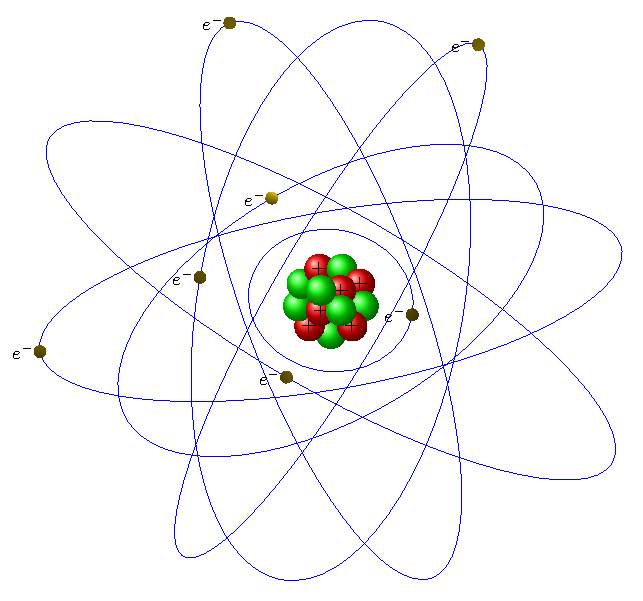
\includegraphics[scale=0.75]{./figuren/introduction}
\end{figure}
Het atoom,  tot begin 19e eeuw bekend als de kleinste bouwsteen van het universum, werd later door Ernest Rutherford \cite{rutherford} ontwaard als zijnde een kern met rondom een wolk van elektronen, negatieve elementaire deeltjes. Elementair in de zin dat ze, voor zover we weten, niet uit kleinere deeltjes bestaan en dus als puntdeeltjes worden beschouwd. Rutherford concludeerde uit zijn verstrooiingsexperimenten dat deze kern ruwweg $10^4$ keer kleiner is dan het atoom. Daar de elektronen puntdeeltjes zijn, kan gezegd worden dat het atoom dus vooral leeg is. De kern van een atoom werd ontleed als een zelf-gebonden systeem van fermionen, deeltjes met halftallige spin, waarbij we een onderscheid kunnen maken tussen ongeladen neutronen en positief geladen protonen. Het zijn de protonen die voor de elektromagnetische binding van de elektronen, ook fermionen, zorgen. In tegenstelling tot elektronen zijn protonen en neutronen, die onder de gezamenlijke term van nucleonen vallen,  geen elementaire deeltjes, maar uit quarks samengestelde systemen. Deze laatste zijn gekend als elementaire deeltjes die met elkaar interageren via de sterke wisselwerking, \'{e}\'{e}n van de vier fundamentele wisselwerkingen van de natuur. In deze thesis beschouwen we de kern samengesteld uit nucleonen en abstraheren we de onderliggende dynamiek van de quarks. Deze abstractie is mogelijk zolang we werken op energieschalen karakteristiek voor een kern, namelijk kleiner dan 1 GeV. Gaan we naar hogere energie\"{e}n dan wordt de structuur van de nucleonen belangrijk. Daar de fundamentele interacties werken tussen elementaire puntdeeltjes, is het niet duidelijk hoe de wisselwerking tussen nucleonen,  de nucleon-nucleon (NN) interactie genaamd, er uitziet. Teneinde dit probleem te benaderen, wordt gebruik gemaakt van effectieve interacties tussen nucleonen. Op basis van een aantal fysische restricties kan een algemene effectieve potentiaal worden opgesteld waarvan de vrijheidsgraden vastgelegd worden door NN verstrooiingsexperimenten. In het algemeen zijn deze interacties vrij complex en nog niet helemaal begrepen. Een kwantummechanisch probleem met veel deeltjes die interageren via een complexe wisselwerking is onmogelijk exact op te lossen en ook met bepaalde benaderingen is dit nog steeds niet evident. In het eenvoudigste model kan een kern benaderd worden door een Fermi-gas van nucleonen  \cite{povh2008particles}. In dit model beschouwen we de kern als een niet-interagerend kwantumgas in een volume dat overeenkomt met het volume van een kern. Voor een schatting van de straal $R$ van een kern kan men gebruik maken van de fenomenologische formule $R=1.2 A^{1/3}$ fm, waarbij $A$ het aantal nucleonen in de kern voorstelt \cite{povh2008particles}. De relevante afstandsschaal is dus van de orde $1$ fm voor de lichtste kernen en $10$ fm voor de zwaarste. Gebruik makende van het onzekerheidsbeginsel van Heisenberg $\Delta x \Delta p \geq \hbar/2$ toont dat de relevante schaal van de impuls in een kern van de orde 10 tot 100 MeV/c is en de bijhorende temperatuur $10^8\ K$ tot $10^{10}\ K$ . Daar de omgevingstemperatuur op aarde rond $300\ K$ ligt, kunnen we aannemen dat de nucleonen de $A$ laagste toestanden bezetten. Het hoogst gevulde energieniveau heet dan het Fermi-niveau en de geassocieerde impuls met deze toestand is de Fermi-impuls. Dit eenvoudige model leent zich ertoe een schatting te maken van enkele grootheden. Zo wordt de dichtheid van de kern en de relatie met de Fermi-impuls:
\begin{equation}
\rho = \frac{A}{V} = 0.14 fm^{-3} =  \frac{2}{3\pi^2 \hbar^3} p^3_F.
\end{equation}
Dit geeft dan een Fermi-impuls $p_F \approx 250\ MeV/c$ waaruit een gemiddelde kinetische energie $\langle T \rangle = 21\ MeV$ volgt. Dit eenvoudig model is slechts goed voor een schatting van grootheden want het houdt geen rekening met de specifieke eigenschappen van het systeem. Zo is de gemiddelde kinetische energie bijvoorbeeld dezelfde voor alle kernen.
In de late jaren 1940 introduceerden Maria Goeppert Mayer en J. Hans D. Jensen onafhankelijk van elkaar de schillenstructuur in kernen \cite{mayer,jensen}. Deze structuur was onder meer succesvol in het verklaren van de zogenaamde magische getallen, zijnde bepaalde aantallen van neutronen en protonen waarbij de kern een verhoogde stabiliteit heeft. 
Het eenvoudigste model dat deze schillenstructuur reproduceert, is het onafhankelijke-deeltjes model (ODM). Hierbij wordt aangenomen dat nucleonen bewegen in individuele orbitalen als gevolg van een potentiaal die de gemiddelde interactie in de kern voorstelt. Correlaties tussen de nucleonen worden hier dus verwaarloosd. Nu kunnen we ons de vraag stellen of nucleonen in een globale potentiaal \"{u}berhaupt een goede benadering is voor een kern. 
In tegenstelling tot het systeem van elektronen in het atoom, dat goed beschreven wordt in een ODM met externe potentiaal afkomstig van de kern, is er in het systeem van nucleonen geen externe materie die een potentiaal genereert. De externe potentiaal inwerkend op een nucleon zou dus het gevolg zijn van interacties met andere nucleonen, het systeem is zelf-gebonden. Dat het netto effect van alle interacties bij benadering beschreven kan worden met een extern veld is niet evident. De verantwoording voor het gebruik van dit model vindt men in paragraaf \ref{verantwoording}. 
Het doel van deze thesis is kennis te verwerven over de eigenschappen van een kern en in het bijzonder over de impulsdistributies van nucleonen, die beschrijven hoe de impuls van de nucleonen in de kern is verdeeld. Ze laten ook toe de verwachtingswaarden te berekenen van operatoren die een functie zijn van de impuls. Zo bepalen we de gemiddelde kinetische energie van de neutronen en protonen aan de hand van de \'{e}\'{e}ndeeltjes impulsdistributie.
Impulsdistributies kunnen gebruikt worden als input bij experimenten waarbij detectie gebeurt via interactie van een deeltje met een kern waarbij een boson, deeltje met heeltallige spin, wordt uitgewisseld. Hoe hoger de impuls van het uitgewisselde deeltje, hoe meer structuur van de kern dit deeltje kan zien. Bij lage inkomende impuls (van de orde 100 MeV en lager) wordt een deeltje aan de volledige kern verstrooid en zijn er weinig effecten van de interne structuur van de kern. Bij hogere inkomende impuls (orde 0.2 GeV en meer) gebeurt verstrooiing echter aan enkelvoudige nucleonen, die een zekere impuls bezitten. Het is duidelijk dat bij detectie van deeltjes met voldoende hoge impuls de impulsdistributies van de nucleonen in kernen in de detectoren moeten gekend zijn om bijvoorbeeld werkzame doorsneden te berekenen. Het Long-Baseline Neutrino Experiment (LBNE \cite{anderson2012first}) maakt gebruik van vloeibare-argon detectoren om eigenschappen van neutrino's met hoge precisie te meten. Een optimale detectie vereist een goede kennis van de neutrino-argon werkzame doorsnede. Daar \textit{Ankowski et al.}\cite{ankowski2014} melden dat er weinig theoretische studies zijn van de impulsdistributies voor $\nuclide[40][18]{Ar}$, onderzoeken we ook deze kern. 
In deze thesis bestuderen we ook tweedeeltjes impulsdistributies in functie van de relatieve impuls van twee nucleonen, de impuls van hun massacentrum en de hoek tussen deze twee impulsen. 
Ten slotte worden de Wignerdistributies \cite{wigner1932quantum} gerelateerd aan de \'{e}\'{e}ndeeltjes impulsdistributies uitgerekend. Deze geven een beeld van de faseruimte in een kwantumsysteem. Via de Weyl-transformatie (cfr. hoofdstuk \ref{hfdstk:wigner}) kunnen operatoren omgezet worden naar functies van positie en impuls, zoals observabelen in de klassieke, niet-kwantum fysica. Met de Wignerdistributie kan de verwachtingswaarde van deze operator berekend worden op dezelfde manier als dit in de klassieke fysica gebeurt, met andere woorden het Wigner-Weyl formalisme laat toe de mathematische methoden uit de klassieke fysica te gebruiken die vaak eenvoudiger zijn dan het kwantummechanische analogon.

\pagebreak
\chapter{Het onafhankelijke-deeltjes model}
\section{Verantwoording} \label{verantwoording}

Dat een ODM een goede benadering is voor een atomaire kern is niet evident. De nucleonen in de kern interageren namelijk met elkaar via de NN kracht die afstotend is op korte afstand en attractief op lange afstand. Na\"{i}ef zou men dus verwachten dat een systeem van nucleonen zich gedraagt als een vloeistof van harde sferen die tegen elkaar stuiteren en een zwakke interactie op middellange afstand ondervinden. Omdat een kern echter uit fermionen bestaat geldt het uitsluitingsprincipe van Pauli dat zegt dat twee identieke fermionen niet dezelfde toestand kunnen bezetten. Hierdoor wordt het botsen van nucleonen onderdrukt, er zijn namelijk geen vrije orbitalen bij lage energie beschikbaar waar de nucleonen na interactie in terecht kunnen komen, met uitzondering van de nucleonen in de hoogst bezette toestanden die naar een leeg orbitaal kunnen verstrooien. Ter illustratie van een model waarbij botsingen verwaarloosd worden beschouwen we eerst een NN potentiaal van de vorm
\begin{equation}
V(\vec{r}_1, \vec{r}_2) = V_0 \  f(\vec{r}_1 - \vec{r}_2).
\end{equation}
Hierbij is $V_0$ de centrale diepte van de potentiaalput en de functie $f$ is van korte dracht en continu. De korte dracht volgt uit de vaststelling dat een nucleon niet interageert met alle andere nucleonen in de kern, een fenomeen gekend als de saturatie van de NN interactie die we illustreren in Figuur \ref{fig:bindings_energie}. Een fysische interactie is alleen afhankelijk van de relatieve vector tussen twee interagerende deeltjes, want een afhankelijkheid van het massacentrum zou translatie-invariantie schenden.
\begin{figure}
\centering 
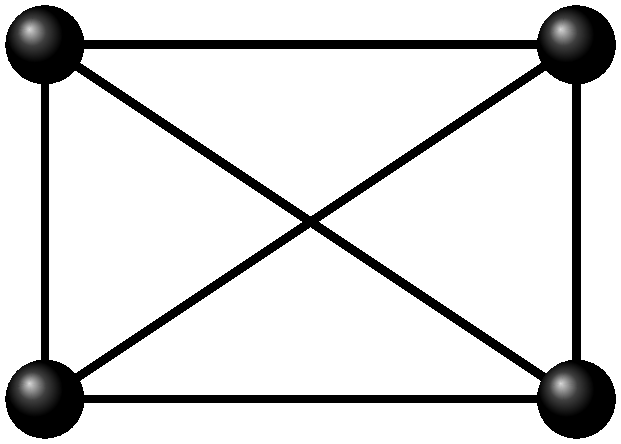
\includegraphics[scale=0.55]{./figuren/saturation}
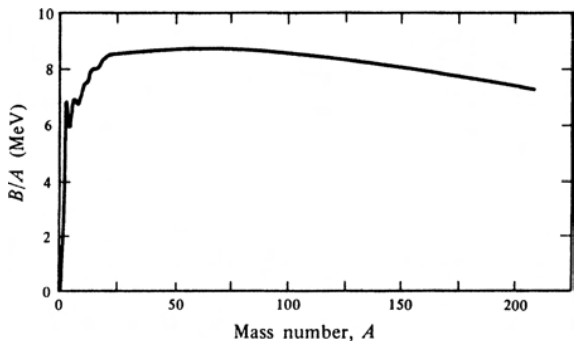
\includegraphics[scale=0.45]{./figuren/binding_energy.png}
\caption{Links: Beschouwen een kern met vier nucleonen, $A = 4$. Als elk nucleon met alle andere nucleonen in de kern interageert dan zijn er $4(4-1)/2$ interacties en is de bindingsenergie ($B$) proportioneel met $A(A-1)$. Voor zware kernen zou dan bij benadering gelden dat $B \propto A^2$. Rechts: Bindingsenergie per nucleon ($B/A$) als functie van $A$ \cite{henley}. Het is duidelijk dat een nucleon slechts interageert met een beperkt aantal andere nucleonen in de kern, m.a.w het aantal interacties per nucleon satureert. Vooral bij zwaardere kernen valt dit op.}
\label{fig:bindings_energie}
\end{figure}
Men kan nu een schatting maken van de centrale potentiaal gevoeld door nucleon 1 door uit te middelen over alle nucleonen interagerend met dit nucleon, gekend als een gemiddeld-veld benadering (GV):
\begin{equation}
V(\vec{r}_1)  = V_0 \int d\vec{r}_2 \ f(\vec{r}_1 - \vec{r}_2) \ \rho (\vec{r}_2).
\end{equation}
Als de dracht van $f$ kort genoeg is kan $\rho (\vec{r}_2)$ benaderd worden door $\rho (\vec{r}_1)$. $V(\vec{r}_1)$ wordt dan
\begin{equation}
V(\vec{r}_1)  = C\  V_0  \ \rho (\vec{r}_1),
\end{equation} 
met $C = \int d\vec{r}_2\ f(\vec{r}_1-\vec{r}_2)$.
In een ODM  is de potentiaal gevoeld door een nucleon in de kern dus evenredig met de dichtheidsdistributie van de kern. Uit \cite{povh2008particles} weten we dat een Fermi-functie een goede benadering is voor de dichtheidsdistributie van een kern:
\begin{equation}
\rho (r) = \frac{\rho_0}{1+\exp{(r-c)/a}}.
\end{equation}
Hierbij is $c$ de straal waarbij de distributie de helft is van zijn maximale waarde en $a$ de spreiding van het interval waarover de distributie afneemt. Daar deze distributie geen hoekafhankelijkheden bevat, impliceert dit sferische symmetrie. Deze aanname wordt ondersteund door de vaststelling dat de quadrupoolmomenten en hogere orde momenten klein zijn voor atomaire kernen in de buurt van de magische getallen \cite{symmetry_shape}. 
Uit deze dichtheidsdistributie volgt dan de Woods-Saxon (WS) potentiaal \cite{povh2008particles}:
\begin{equation} \label{eq:ws_potential}
V(r)  = \frac{V_{WS}  }{1+\exp{(r-c)/a}}.
\end{equation}
De Schr\"{o}dingervergelijking voor dergelijke potentiaal heeft geen analytische oplossing tenzij we deze potentiaal benaderen met een sferische harmonische oscillator (HO) potentiaal 
\begin{equation} \label{eq:HO_potential}
V_{HO}(r) = \frac{1}{2} M_N (\omega r)^2- V_0,
\end{equation}
waarbij $M_N$ de nucleonmassa voorstelt en $V_0$ een parameter die we zodanig kiezen dat een goede benadering van de WS potentiaal wordt bekomen. Echter, bij het oplossen van de Schr\"{o}dingervergelijking stellen we deze laatste constante gelijk aan nul voor eenvoudigheid, het is slechts een verschuiving van de energieschaal. Een goede parametrisatie van $\hbar \omega$ \cite{maarten} wordt gegeven door
\begin{equation} \label{eq:omega}
\hbar\omega (MeV) = \frac{45}{A^{1/3}}-\frac{25}{A^{2/3}},
\end{equation}
waarbij $A$ het aantal nucleonen is in de kern. Figuur \ref{fig:hows} laat zien dat dit een relatief goede benadering is. Daar het gemiddeld veld interagerend met een nucleon wordt bepaald door de $A-1$ andere nucleonen moet de breedte van de externe potentiaal afhankelijk zijn van $A$. Daar de straal van kernen vergroot met aantal nucleonen verwacht men dat de oscillator potentiaal steeds breder wordt als $A$ groter wordt. Dat deze potentiaal naar oneindig gaat voor een steeds groter wordende straal is niet fysisch want nucleonen worden verondersteld de kern te kunnen verlaten als ze voldoende energie hebben. Daar we alleen de grondtoestand van kernen beschouwen speelt deze niet-fysische factor hier geen rol.

\begin{figure}
\centering
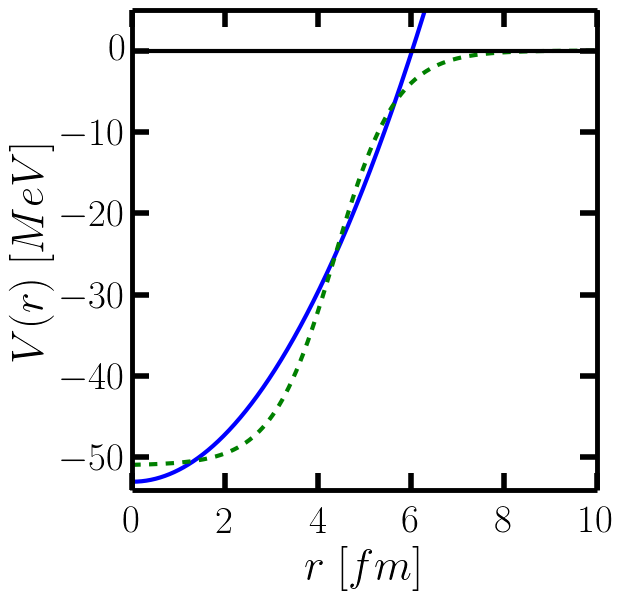
\includegraphics[scale=0.4]{./figuren/potentiaal_vgl.png}
\caption{Vergelijking van verschillende GV-potentialen voor argon ($A= 40$). De gestreepte groene curve stelt een WS potentiaal voor, gegeven door uitdrukking \eqref{eq:ws_potential}, met $V_{WS} = -51$ MeV, $c=1.2$ fm en $a= 0.67$ fm . De volle blauwe curve is een HO potentiaal, gegeven door uitdrukking \eqref{eq:HO_potential}, waarbij $\omega$ gegeven door \eqref{eq:omega} met $A = 40$ en $V_0= 53$ MeV.}
\label{fig:hows}
\end{figure}

\section{Golffunctie in een sferische harmonische oscillator potentiaal}
Uit al het bovenstaande is het duidelijk de we een kern kunnen benaderen als nucleonen die onafhankelijk van elkaar bewegen in een sferische HO potentiaal die het gemiddeld veld gevoeld door een nucleon als gevolg van alle andere nucleonen voorstelt. De A-deeltjes Hamiltoniaan 
\begin{equation} \label{eq:full_ham}
\hat{H} = \sum_i^A \hat{T}_i + \sum_{\substack{ij \\ i  \neq j}}^A \hat{V}_{ij}  + \sum_{\substack{ijk \\ i \neq k \neq j}}^A \hat{W}_{ijk}  + \cdots ,
\end{equation}
waarbij $\hat{V}_{ij}, \hat{W}_{ijk}$ respectievelijk tweedeeltjes en driedeeltjes interacties zijn en $\hat{T}_i$ de kinetische energie operator is, vereenvoudigt zich dan tot
\begin{equation} \label{eq:full_ham2}
\hat{H} = \sum_i^A \left(\hat{T}_i + \hat{V}^{HO} \right).
\end{equation}
De nieuwe Hamiltionaan is een som van \'{e}\'{e}ndeeltjes Hamiltonianen die een interactie met een extern veld bevatten voorgesteld door $ \hat{V}^{HO}$. Een GV benadering zorgt dus voor een reductie tot een probleem van \'{e}\'{e}n deeltje:
\begin{equation} \label{eq:HO}
\left( -\frac{\hbar^2}{2M_N} \nabla^2 + \frac{1}{2} M_N \omega^2 r^2 \right) \psi_{nlm}(\vec{r}) = E_{nl}\ \psi_{nlm}(\vec{r}).
\end{equation}
De kern-afhankelijke $\omega$ wordt vastgelegd door \eqref{eq:omega}. Eigenfuncties hebben een radi\"{e}el kwantumgetal $n$ en een impulsmoment $l$ met projectie $m$.
Oplossingen van bovenstaande differentiaalvergelijking kunnen als gevolg van de sferische symmetrie van de HO potentiaal worden opgesplitst in een radi\"{e}el en een hoekafhankelijk deel:
\begin{equation} \label{eq:solution_ho}
\psi_{nlm}(\vec{r}) \equiv \braket{\vec{r}|nlm} = R_{nl}(r)Y_{lm}(\Omega),
\end{equation}
waar $Y_{lm}(\Omega)$ de sferische harmonieken voorstellen. Het radi\"{e}le deel van de golffunctie in functie van de gegeneraliseerde Laguerre-polynomen $L^\alpha_n(r)$ wordt gegeven door
\begin{equation}
 R_{nl}(r) = \left[ \frac{2n!}{\Gamma(n+l+\frac{3}{2})}\nu^{l+\frac{3}{2}} \right]^{\frac{1}{2}} r^l e^{-\frac{\nu r^2}{2}} L^{l+\frac{1}{2}}_n(\nu r^2),
\end{equation}
waarbij
\begin{equation}
\nu \equiv \frac{M_N \omega}{\hbar}.
\end{equation}

De energie eigenwaarden zijn onafhankelijk van kwantumgetal $m$ als gevolg van de sferische symmetrie:
\begin{equation} \label{eq:energie_HO}
E_{nl} = \hbar \omega \left(2n+ l + \frac{3}{2} \right).
\end{equation} 
Een handige notatie wijst letters toe aan de verschillende $l$-waarden. Zo wordt de toestand met $n = 0$ en $l = 1$ geschreven als $0p$. De $l$-waarden 0, 1, 2, 3, 4, 5, 6 worden respectievelijk genoteerd als $s,p,d,f,g,h$.
Uit formule \eqref{eq:energie_HO} blijkt de HO potentiaal een ontaarding te hebben die dus bijgevolg een vrijheid laat bij het opvullen van de orbitalen. Een realistischer potentiaal, zoals een Woods-Saxon potentiaal, heeft deze vrijheid niet en elk niveau $nl$ heeft een verschillende energie. Om dit probleem te illustreren kijken we naar de $1s$ en $0d$ toestanden in een HO. De energie gegeven door vergelijking \eqref{eq:energie_HO} is voor beide toestanden dezelfde, namelijk $E = \frac{7}{2} \hbar\omega$ en het is dus onduidelijk welke toestand er eerst bezet wordt. Om deze ontaarding te vermijden gebruiken we de opvulling van een Woods-Saxon potentiaal. Hoe gebeurt de opvulling dan?  Figuur \ref{fig:ho_waves} geeft aan dat toestanden van de harmonische oscillator met een hoog impulsmoment $l$ zich met grotere waarschijnlijkheid verder van het centrum van de kern begeven dan toestanden met kleinere $l$. De WS potentiaal is dieper dan de HO potentiaal op grote afstand van het centrum en minder diep op kleine afstand (Figuur \ref{fig:hows}). Dus toestanden met grote $l$ voelen een diepere potentiaal en schuiven dus naar lagere energie\"{e}n. 
Zoals reeds vermeld in de inleiding is de verklaring van de magische getallen \'{e}\'{e}n van de grootste successen van het schillenmodel. Een ODM zoals hierboven is opgesteld kan deze magische getallen echter nog niet verklaren. Een  spin-baan potentiaal, een gemiddeld veld afkomstig van de individuele spin-baan interacties in de NN potentiaal, gegeven door
\begin{equation}
V_{ls} = C_{ls}\  \vec{l} \cdot \vec{\sigma} =  \frac{ C_{l\sigma}}{2} \left( j^2 - l^2 - \sigma^2 \right),
\end{equation}
zorgt voor gedeeltelijke opheffing van de ontaarding van de energieniveaus. 
\begin{figure}
\centering
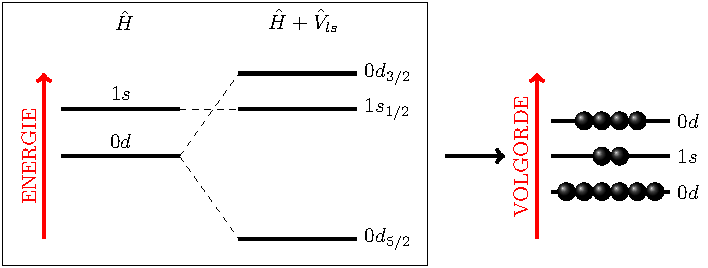
\includegraphics[scale=1]{./figuren/opvulling}
\caption{Links: invloed van een spin-baan interactie op de eigentoestanden $1s$ en $0d$ van de Hamiltoniaan met een Woods-Saxon potentiaal. Rechts: volgorde waarin we toestanden bezetten in de harmonische oscillator potentiaal.}
\label{fig:spin_orbit}
\end{figure}
Energietoestanden worden dan afhankelijk van het totaal impulsmoment, $\vec{j} = \vec{l} + \vec{\sigma}$ waarbij $\vec{l}$, $\vec{\sigma}$ respectievelijk het orbitaal en spin impulsmoment zijn. Daar de kern alleen fermionen bevat is $\abs{\vec{\sigma}} = \frac{1}{2}$. Spin-baan koppeling zorgt dan voor een verschuiving in energie waarbij toestanden met $j = l + 1/2$ een lagere energie krijgen tegenover de toestand zonder spin-baan koppeling en toestanden met $j = \abs{l - 1/2}$ steeds een hogere energie (Figuur \ref{fig:spin_orbit}). Deze extra term in de Hamiltoniaan zorgt er echter voor dat de oplossingen van de Schr\"{o}dingervergelijking geen analytische uitdrukking meer hebben. Om deze spin-baan koppeling enigszins te verwerken in ons model gebeurt de opvulling van de toestanden in de volgorde vastgelegd door een model die deze wel bevat. Omdat toestanden nog steeds een goed gedefinieerd kwantumgetal $l$ hebben kunnen we de opvulling gebruiken van een Woods-Saxon potentiaal met spin-baan koppeling waarbij het kwantumgetal $j$ slechts wordt gebruikt als een label van de toestanden. Dan gebeurt de opvulling zoals in Figuur \ref{fig:spin_orbit}. Het zijn echter de golffuncties van de harmonische oscillator \eqref{eq:solution_ho} die gebruikt worden. We kunnen dus concluderen dat door de spin-baan koppeling het aantal nucleonen in de hoogst gevulde orbitalen zal wijzigen en er soms orbitalen worden bezet die zonder spin-baan niet bezet zouden zijn. Een volledig schema van de opvulling in een WS potentiaal wordt getoond in Figuur \ref{fig:WS_opvulling}.

\begin{figure}[H]
\centering
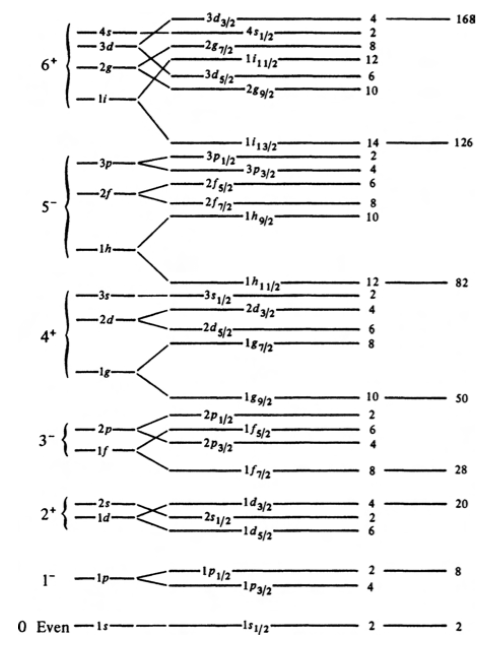
\includegraphics[scale=0.55]{./figuren/opvulling_WS.png}
\caption{Energieschema van individuele orbitalen in een Woods-Saxon potentiaal uit \cite{henley}.}
\label{fig:WS_opvulling}
\end{figure}

\begin{figure}[H]
\centering
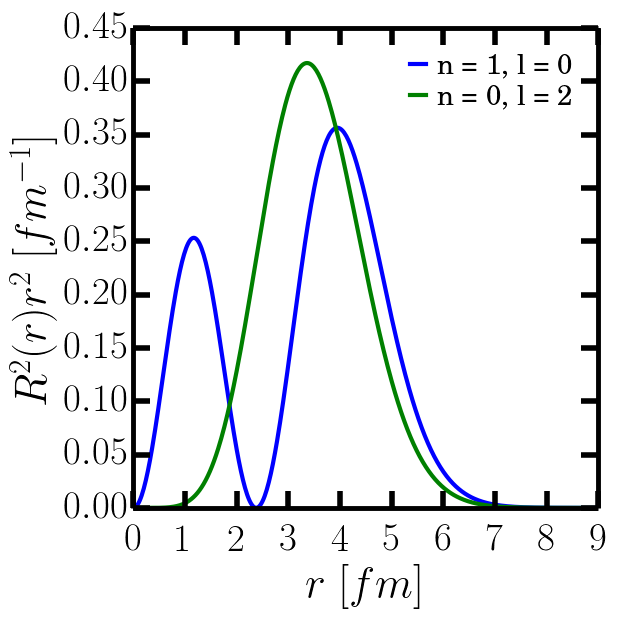
\includegraphics[scale=0.43]{./figuren/waves.png}
\caption{De probabiliteitsdistributie $R^2(r)r^2$ voor twee ontaarde toestanden in de harmonische oscillator  ($E = \frac{7}{2} \hbar \omega$). De beschouwde kern is argon ($A= 40$).}
\label{fig:ho_waves}
\end{figure}





\chapter{E\'{e}ndeeltjes impulsdistributie} \label{eendeeltjes}
\section{Algemene kenmerken}

Nucleonen opsluiten in een kleine ruimte - klein in de zin dat het onzekerheidsbeginsel van Heisenberg ($\Delta x \Delta p \geq \hbar/2$) merkbaar is - zorgt ervoor dat deze nucleonen een zekere kinetische energie krijgen, die dus geassocieerd is met de lokalisatie van de nucleonen. We verwachten dus dat een nucleon een zekere impuls bezit die verdeeld is volgens een bepaalde impulsdistributie. Impulsdistributies spelen een belangrijke rol in verstrooiingsexperimenten aan kernen als de uitgewisselde impuls voldoende hoog is. Daar de dimensies van een nucleon van de orde $\approx$ 0.8 fm zijn, verstrooit het inkomend deeltje aan een enkel nucleon in de kern als de uitgewisselde impuls van $0.2$ GeV of hoger. Dit fenomeen heet quasi-elastische verstrooiing. Via quasi-elastische verstrooiingsexperimenten waarbij het verstrooide nucleonen de kern verlaat kan men de initi\"{e}le impuls bepalen van het verstrooide nucleon via behoud van energie en impuls, dus ook de \'{e}\'{e}ndeeltjes  impulsdistributie \cite{kobayashi}. In deze thesis berekenen we de impulsverdelingen van nucleonen op basis van een ODM.
Algemeen wordt de kans om een deeltje te vinden met een momentum in het interval $[k,k+dk]$ gegeven door $n^{[1]}(k) k^2dk$ met

\begin{equation} \label{eq:one_patricle_distr}
	n^{[1]}(k)=\int d\Omega_k\ n^{[1]}(\vec{k}),
\end{equation}
waarbij
\begin{equation} 
	n^{[1]}(\vec{k})=\frac{1}{(2\pi)^3}\int d\vec{r}_1 \int d\vec{r}_1^{\ \prime} e^{i\vec{k}\cdot (\vec{r}_1-\vec{r}^{\ \prime}_1)}\rho_1(\vec{r}_1,\vec{r}_1^{\ \prime})
\end{equation}
de \'{e}\'{e}ndeeltjes impulsdistributie voorstelt. Hierbij is

\begin{equation}
\rho_1(\vec{r}_1,\vec{r}^{\ \prime}_1) = \int \{d\vec{r}_{2-A}\} \Psi^*_A(\vec{r}_1,\vec{r}_2,\vec{r}_3, ... ,\vec{r}_A)\Psi_A(\vec{r}_1^{\ \prime},\vec{r}_2,\vec{r}_3, ... ,\vec{r}_A).
\end{equation}


de \'{e}\'{e}ndeeltjes niet-diagonale dichtheidsmatrix (ENDM) en $\Psi_A(\vec{r}_1,\vec{r}_2,\vec{r}_3, ... ,\vec{r}_A)$ stelt de grondtoestand van een nucleus met A nucleonen voor. We maakten gebruik van de volgende notatie:

\begin{equation}
\{d\vec{r}_{i-A}\}  = d\vec{r}_i d\vec{r}_{i+1}...\vec{r}_A.
\end{equation}
 


Als $\braket{\Psi_A|\Psi_A}=1$, heeft men dat 


\begin{equation}
\int d\vec{k} \ n_1(\vec{k})= 1.
\end{equation}
Dit is niets anders dan de totale kans om $A$ nucleonen te vinden in de kern. Het diagonaalelement $\rho_1(\vec{r},\vec{r}) \equiv \rho(\vec{r}) $ is dan de dichtheid van de nucleonen op positie $\vec{r}$.

In het tweedekwantisatie formalisme (voor conventies zie Appendix \ref{sec:tweede_kwant}) kan men de  \'{e}\'{e}ndeeltjes impulsdistributie schrijven als
\begin{equation}
n^{[1]}(\vec{k})= \frac{1}{A}\bra{\Psi_A} \psi^\dagger(\vec{k}) \psi(\vec{k})\ket{\Psi_A}.
\end{equation}
De operator die hier ge\"{e}valueerd wordt is een teloperator het aantal nucleonen met impuls $\vec{k}$ geeft en wordt voorgesteld in Figuur \ref{fig:feyn}. Het bewijs voor deze uitdrukking wordt gegeven in Appendix \ref{operator}.   
\begin{figure} [h]
\centering
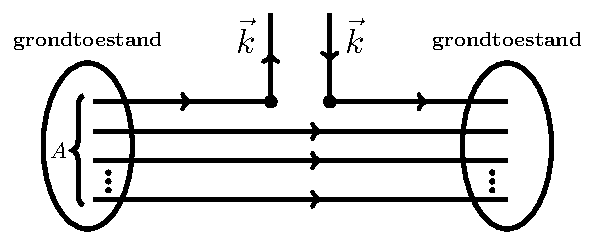
\includegraphics[scale=1]{./figuren/ob_feynman}
\caption{Feynmandiagram van de  \'{e}\'{e}ndeeltjes impulsoperator. De operator annihileert en cre\"{e}ert een nucleon met momentum $\vec{k}$ op hetzelfde tijdstip, zo is er geen energiestroom. De initi\"{e}le en finale toestand zijn dan dezelfde.}
\label{fig:feyn}
\end{figure}

Op een analoge manier kan de ENDM in het tweedekwantisatie formalisme geschreven worden als
\begin{align}
\rho(\vec{r}_1,\vec{r}^{\ \prime}_1) & =  \int \{d\vec{r}_{2-A}\} \Psi^*_A(\vec{r}_1,\vec{r}_2,\vec{r}_3, ...,\vec{r}_A)\Psi_A(\vec{r}_1^{\ \prime},\vec{r}_2,\vec{r}_3, ... ,\vec{r}_A)   \nonumber \\
& = \frac{1}{A!} \int \{d\vec{r}_{2-A}\} \braket{\Psi_A|\psi^\dagger(\vec{r}_1) \psi^\dagger(\vec{r}_2) ...\psi^\dagger(\vec{r}_A) \psi(\vec{r}_{A-1}) ...  \psi(\vec{r}_2)\psi(\vec{r}_1^{\ \prime})|\Psi_A }  \nonumber  \\
& = \frac{1}{A}\braket{\Psi_A|\psi^\dagger(\vec{r}_1) \psi(\vec{r}_1^{\ \prime})|\Psi_A }.
\end{align}
Hier annihileert $\psi^\dagger(\vec{r}_1) \psi(\vec{r}_1^{\ \prime})$  een nucleon op positie $\vec{r}_1^{\ \prime}$ en cre\"{e}ert een nucleon op positie  $\vec{r}_1$. De diagonaaloperator $\psi^\dagger(\vec{r}_1) \psi(\vec{r}_1)$ is een teloperator in de configuratieruimte die het aantal nucleonen op positie $\vec{r}_1$ telt.





\subsubsection{E\'{e}ndeeltjes impulsdistributie in een harmonische oscillator potentiaal}
Een ODM veronderstelt dat een nucleon beweegt in het gemiddelde veld van alle andere nucleonen. Omdat er geen interacties zijn tussen de deeltjes, en dus ook geen correlaties, is de totale golffunctie slechts een product van \'{e}\'{e}ndeeltjesgolffuncties van de nucleonen. Aangezien nucleonen fermionen zijn, en dus voldoen aan het uitsluitingsprincipe van Pauli, moet de totale golffunctie antisymmetrisch zijn onder elke permutatie van twee nucleonen. De golffunctie krijgt dan de gedaante van een Slaterdeterminant van de \'{e}\'{e}ndeeltjesgolffuncties:
\begin{equation} \label{eq:slater}
\Psi_A(\vec{r}_1,\vec{r}_2,\vec{r}_3, ... ,\vec{r}_A)= \frac{1}{\sqrt{A!}} \sum^A_{\substack{i_1 i_2 \ldots i_A}} 
													  \varepsilon_{i_1 i_2 \ldots i_A} \phi_{i_1}(\vec{r}_1)
													         \phi_{i_2}(\vec{r}_2)...
													         \phi_{i_A}(\vec{r}_A).
\end{equation}

Hierbij is $\varepsilon_{i_1 i_2 \ldots i_A}$ de totaal antisymmetrische Levi-Civita tensor en de sommaties over de indices $i_1,\ldots ,i_A$  gaan over alle bezette \'{e}\'{e}ndeeltjestoestanden in de grondtoestand van de kern. De \'{e}\'{e}ndeeltjesgolffuncties voldoen aan de orthonormaliteitsregel:
\begin{equation} \label{eq:orthogonality}
\int d\vec{r}_i\  \phi^*_l(\vec{r}_i)\phi_m(\vec{r}_i) = \delta_{lm}.
\end{equation}

Gebruik makende van deze eigenschap wordt de ENDM 
\begin{align} \label{eq:1pmd}
\rho_1(\vec{r}_1,\vec{r}^{\ \prime}_1) = \frac{1}{A}\sum_{\substack{i}} \phi^*_i(\vec{r}_1) \phi_i(\vec{r}_1^{\ \prime}).
\end{align}

Met de definitie van de golffunctie in de impulsruimte als de Fouriergetransformeerde van de golffunctie in de configuratieruimte,
\begin{equation} \label{eq:fourier}
\phi_i(\vec{k}) = \frac{1}{(2\pi)^{3/2}} \int d\vec{r} e^{-i\vec{k}\cdot \vec{r}} \phi_i(\vec{r}),
\end{equation}
wordt \eqref{eq:one_patricle_distr}:
\begin{align} \label{eq:ob_mf}
n^{[1]}(\vec{k})&=\frac{1}{A(2\pi)^3} \sum_{\substack{i}} \int d\vec{r}_1 \int d\vec{r}_1^{\ \prime} e^{i\vec{k}\cdot (\vec{r}_1-\vec{r}^{\ \prime}_1)}
	\phi^*_i(\vec{r}_1)\phi_i(\vec{r}_1^{\ \prime})\nonumber \\
	& = \frac{1}{A} \sum_{\substack{i}} \phi^*_i(\vec{k})\ \phi_i(\vec{k}) \nonumber\\
	& = \frac{1}{A} \sum_{\substack{i}} \ \abs{\phi_i(\vec{k}) }^2.
\end{align}
De golffuncties in de impulsruimte kunnen berekend worden via Fouriertransformatie \eqref{eq:fourier} van de golffuncties in de configuratieruimte. Echter, in het geval van een HO potentiaal is het eenvoudiger de Schr\"{o}dingervergelijking (\ref{eq:HO}) in de impulsruimte,
\begin{equation} \label{eq:HO_momentum}
\left( -\frac{M_N \omega^2}{2} \nabla^2 + \frac{\hbar^2}{2M_N} k^2 \right) \tilde{\psi}_{nlm}(\vec{k}) = E\tilde{\psi}_{nlm}(\vec{k}),
\end{equation}
op te lossen. Deze differentiaalvergelijking heeft dezelfde vorm als de Schr\"{o}dingervergelijking in de configuratieruimte, met andere woorden de oplossingen zijn van dezelfde vorm als \eqref{eq:solution_ho}:
\begin{equation} \label{eq:splits_momentum}
\psi_{nlm}(\vec{k}) \equiv \braket{\vec{k}|nlm} = K_{nl}(k)Y_{lm}(\Omega_k)	
\end{equation}
met
\begin{equation} \label{eq:HO_mom_radwave}
 K_{nl}(k) = \left[ \frac{2n!}{\Gamma(n+l+\frac{3}{2})}\nu^{\prime \ l+\frac{3}{2}} \right]^{\frac{1}{2}} k^l e^{-\frac{\nu' k^2}{2}} L^{l+\frac{1}{2}}_n(\nu^{\prime} k^2).
\end{equation}
Hierbij is
\begin{equation}
\nu^{\prime} \equiv \frac{\hbar}{M_N \omega}.
\end{equation}

Nucleonen zijn fermionen, deeltjes met spin $ \frac{\vec{1}}{2}$. De spin van een deeltje heeft een bepaalde projectie langs een gekozen as, we kiezen hier de verticale z-as. Dan kan de projectie naar boven of naar onder zijn en wordt aangegeven door het kwantumgetal $\sigma$ (respectievelijk $\sigma =1/2$ of $-1/2$). Om een onderscheid te maken tussen protonen en neutronen maken we gebruik van het isospin kwantumgetal $\tau$. Beiden hebben isospin $\vec{I}= 1/2$ maar protonen krijgen projectie $\tau = + 1/2$ en neutronen $\tau = - 1/2$. De totale golffunctie in de impulsruimte van een deeltje in een sferische HO potentiaal wordt dan gegeven door
\begin{equation}
\phi_\alpha (\vec{k}) = \psi_{n_\alpha l_\alpha m_\alpha}(\vec{k}) \chi_{\sigma_\alpha}  \xi_{\tau_\alpha}
\end{equation}
waarbij $\psi_{n_\alpha l_\alpha m_\alpha}(\vec{k})$ de HO golffunctie in de impulsruimte is, gegeven door \eqref{eq:splits_momentum}. Hier zijn $\chi_{\frac{1}{2}\sigma_\alpha} $ zijn spinspinoren gedefinieerd als
\begin{equation}
\chi_{+1/2} = \begin{pmatrix} 1\\ 0 \end{pmatrix}, \qquad \chi_{-1/2} = \begin{pmatrix} 0\\ 1 \end{pmatrix}.
\end{equation}
Analoge definities gelden voor isospinspinoren $\xi_{\tau_\alpha}$ .
Integratie over alle hoekafhankelijkheid $\Omega_k$ leidt tot een distributie van de grootte van de impuls:
\begin{align} \label{eq:ob_magnitude}
n^{[1]}(k) &  =  \frac{1}{A} \int d\Omega_k \sum_{\tau nlm\sigma}\ \psi^*_{n l m}(\vec{k})\psi_{n l m}(\vec{k}) \ \chi^*_{\sigma} \chi_{\sigma}\ \xi^*_{\tau}  \xi_{\tau} \nonumber\\
& =  \frac{2}{A} \sum_{\tau }  \sum_{ nl }(2l+1) \gamma_{nl}K^2_{nl}(k).
\end{align}
Hier corrigeert $\gamma_{nl}$ voor niet volledig gevulde niveaus en is net als de golffunctie (door  afhankelijkheid van $\nu$) kernafhankelijk. Bijvoorbeeld bij  $\nuclide[12][]{C}$ is het niveau $nl = 0p$ voor protonen en neutronen maar voor $4/6$ gevuld en bijgevolg is $\gamma _{0p}= 4/6$. Daar kernen een verschillend aantal protonen en neutronen kunnen bezitten zijn de bovengrenzen van sommaties over $n,l$ afhankelijk van het aantal protonen en neutronen in de beschouwde kern. Dit gezegd zijnde kunnen we ook schrijven dat de \'{e}\'{e}ndeeltjes impulsdistributie de som is van de impulsdistributies van de neutronen en protonen:
\begin{equation}
n^{[1]}(k) = n_n^{[1]}(k) + n_p^{[1]}(k).
\end{equation}

\section{Resultaten}

De berekende \'{e}\'{e}ndeeltjes impulsdistributies $n^{[1]}(k)$ voor verschillende kernen worden getoond in Figuur \ref{fig:oneparticledistr}. Omdat de impulsdistributie in een ODM een som is van de individuele impulsdistributies van elke bezette \'{e}\'{e}ndeeltjestoestand \eqref{eq:ob_mf} zijn ook deze individuele bijdragen tot de totale distributie weergegeven. Uit de resultaten valt op dat de distributies nooit nul worden, dit is volgt uit de eigenschap van de HO golffuncties. De HO potentiaal in de impulsruimte wordt steeds groter voor grotere wordende impuls., maar blijft steeds eindig. Als gevolg hebben de golffuncties steeds een eindige probabiliteit voor $k$ gaande naar oneindig.  Aan de hand van de berekende distributies kan de gemiddelde kinetische energie van nucleonen in een bepaalde kern bepaald worden:
\begin{equation}\label{eq:kin}
\mean{T_N} = \frac{\hbar^2}{2M_N} \frac{ \int dk\ n_N^{[1]}(k)\ k^4}{\int dk\ n_N^{[1]}(k)\ k^2},
\end{equation}
waarbij de index staat voor protonen ($p$) of neutronen ($n$) en we aannemen dat protonen en neutronen dezelfde massa hebben ($M_p = M_n$).
Resultaten voor de gemiddelde kinetische energie \eqref{eq:kin} vindt men in Tabel \ref{tab:kineticenergy}. Vergelijking van de distributies met de waarden berekend in een model met correlaties \cite{maarten} blijkt dat een ODM de waarden goed reproduceert bij lage impuls ($k \lesssim 2.0\ fm^{-1}$) maar naarmate men naar grotere impuls gaat zorgen correlaties voor een brede staart in de distributie. De kinetische energie is gerelateerd aan het vierde moment van de impulsdistributie en daarom dus sterk afhankelijk van de staart van de distributie. Correlaties tussen de nucleonen zorgen dus voor een enorme toename in gemiddelde kinetische energie. Voor een beschrijving met correcties op het GV als gevolg van correlaties verwijzen we naar \cite{ryckebusch2015stylized}.
De waarden in Tabel \ref{tab:kineticenergy} kunnen we verklaren aan de hand van twee effecten die elkaar tegenwerken. Een eerste effect is de invloed van de grootte van de kern, hoe groter de kern des te groter de ruimte waarin een nucleon kan bewegen. Volgens het onzekerheidsbeginsel van Heisenberg volgt dan dat de gemiddelde impuls, en dus ook de kinetische energie lager zal zijn voor nucleonen in een grotere kern. Isotopen van Calcium, $\nuclide[40][]{Ca}$ en $\nuclide[48][]{Ca}$ bezitten bij definitie hetzelfde aantal protonen en in de grondtoestand bezetten deze protonen dus dezelfde toestanden in beide kernen. In $\nuclide[48][]{Ca}$ voelen de protonen echter een bredere potentiaal en ligt hun gemiddelde kinetische energie dus lager dan in $\nuclide[40][]{Ca}$. Een tweede trend in de resultaten is een toename van de gemiddelde kinetische energie als een nieuw energieniveau bezet wordt. Als men bijvoorbeeld naar de gemiddelde kinetische energie van protonen kijkt bij $\nuclide[48][]{Ca}$ en $\nuclide[56][]{Fe}$ dan is deze groter voor de laatstgenoemde. In de grondtoestand van $\nuclide[48][]{Ca}$ zijn te protontoestanden opgevuld tot en met energie $E = 7/2\ \hbar \omega_{A = 48}$ en in $\nuclide[56][]{Fe}$ zijn er nog 6 protonen die een hogere energietoestand bezetten ( $E = 9/2\ \hbar \omega_{A = 56}$) en dus voor een verhoogde gemiddelde kinetische energie zorgen. 
Aangezien we de massa van een neutron en proton als gelijk aannemen is het verschil in kinetische energie van de protonen en neutronen in eenzelfde kern te wijten aan een verschil in aantal bezette toestanden. Naarmate kernen een groter massagetal $A$ hebben verwachten we steeds meer neutronen in verhouding met het aantal protonen (afnemende protonfractie $x_p = Z/A$ ) want voor zwaardere kernen wordt de Coulombafstoting steeds belangrijker. Als het hoogst gevulde energieniveau van de neutronen in een kern een hogere energie heeft dan het hoogst gevulde niveau van de protonen dan is er inderdaad een verschil in kinetische energie.  

In Figuur \ref{fig:oneparticledistr_2} wordt de kans om een $A$ nucleonen te vinden met impuls $k$ getoond in functie van de impuls, deze kans wordt gegeven door $n^{[1]}(k)k^2dk$. 
Het gemiddelde $\mu$ van een van een probabiliteitsdistributie $P(x)$ is gedefinieerd als
\begin{equation}
\mu = \frac{\int_D dx\ xP(x)}{\int_D dx\ P(x)},
\end{equation}
en het $i$de centraal moment als
\begin{equation}
\mu_i \equiv \frac{\int_D dx\ (x-\mu)^i P(x)}{\int_D dx\ P(x)},
\end{equation}
waarbij $D$ het domein is van de distributie. 
Met behulp van deze definities defini\"{e}ren we de variantie $\sigma^2 = \mu_2$. Afwijkingen van een Gaussische (normale) distributie,
\begin{equation} \label{eq:gaussian}
P_{normal}(k)= \frac{1}{\sigma \sqrt{2\pi}} \exp{-\frac{(k-\mu)^2}{2\sigma^2}},
\end{equation}
worden gekarakteriseerd door scheefheid
\begin{equation} \label{eq:skew}
\mathcal{S}  = \frac{\mu_3}{\sigma^3}
\end{equation}
en kurtosis
\begin{equation} \label{eq:kurtosis}
\kappa  = \frac{\mu_4}{\sigma^4} - 3
\end{equation}
die beiden nul zijn voor een normale distributie. De waarden in Tabel \ref{tab:properties}, weergegeven in Figuur \ref{fig:properties} geven aan dat de distributies bij benadering Gaussisch zijn, kurtosis en scheefheid zijn klein. De absolute waarde van de kurtosis groeit naarmate $A$ groter wordt. Een negatieve kurtosis duidt erop dat de distributies minder gepiekt zijn en kleinere staarten hebben dan een Gaussische distributie. Lichte kernen hebben een linkse scheefheid ($\mathcal{S} > 0$) en scheefheid wordt kleiner naarmate we naar zwaardere kernen gaan. De zwaarste kernen hebben rechtse scheefheid ($\mathcal{S} < 0$) in de distributie wat erop duidt dat er meer nucleonen te vinden zijn met een kleiner dan gemiddelde impuls en dat de grootste afwijkingen van de gemiddelde impuls te vinden zijn rechts van het gemiddelde, bij de grootste impulsen. Daar kurtosis en scheefheid beperkt blijven in grootte kunnen we besluiten dat impulsverdeling van nucleonen in een kern bij benadering wordt beschreven een door Gaussische verdeling. Figuur \ref{fig:oneparticledistr_2} geeft naast de berekende impulsdistributie ook een fit van een Gaussische distributie \eqref{eq:gaussian} aan de theoretische curve weer. De parameters $\mu$ en $\sigma$ worden gefit volgens de methode van de kleinste kwadraten.
Weergegeven in de figuur is ook $\chi^2$:
\begin{equation} \label{eq:chisquared}
\chi^2 = \sum_k (n^{[1]}(k)k^2 - P_{normal}(k))^2,
\end{equation}
die de goedheid van de fit weergeeft. De sommatie gaat over $k \in  [0,2]  fm^{-1}$ met een stap van $0.01\ fm^{-1}$. Hoe kleiner $\chi^2$, hoe beter de normale verdeling de theoretische curve benadert. 
De normale verdeling, gedefinieerd in \eqref{eq:gaussian}, heeft de eigenschap dat ze waarden kan aannemen voor een negatief argument. De beschouwde variabele is hier de grootte van de impuls $k$ die slechts gedefinieerd is in het interval $[ 0, + \infty]$. Een Maxwell-Boltzmannverdeling zou een goed alternatief zijn aangezien het een sferisch equivalent is van de normale distributie:
\begin{equation}
P_{MB}(k) \propto k^2 \exp{-\frac{k^2}{2a^2}}
\end{equation} 
met 
\begin{equation}
a= \sqrt{\frac{\pi}{8}}\mu.
\end{equation}
In \cite{PhysRevC.86.044619} is reeds besloten dat een redelijke fit geeft voor lichte kernen en een slechte fit voor de zwaardere kernen in een GV-model met WS potentiaal. Hetzelfde verhaal geldt voor impulsdistributies in een HO potentiaal. De voornaamste reden voor de slechte fit is de negatieve kurtosis (kleinere staarten ten opzichte van normale verdeling) van de berekende impulsdistributies. Een Maxwell-Boltzmannverdeling heeft namelijk een zware staart aan de hoge-impulskant.
Uit de conclusies over de twee bovenstaande fits lijkt het interessant om de functie
\begin{equation} \label{eq:powgauss}
P_{PG}(k) = N_{norm} \times k^\alpha \exp{-\frac{(k-\mu)^2}{2\sigma^2}}
\end{equation} 
te beschouwen waarbij $N_{norm}$, $\alpha$, $\mu$ en $\sigma$ gefit worden volgens de methode van de kleinste kwadraten. Aangezien er geen analytische uitdrukking is voor de integraal $\int dk P_{PG}(k)$ fitten we dus ook een normalisatiefactor $N_{norm}$. We controleren ook of de gefitte curve correct genormaliseerd is op 1. In Figuur \ref{fig:oneparticledistr_3} ziet men dat deze functie een heel goede fit geeft aan onze theoretische curve voor lichte kernen, $\chi^2$ is verwaarloosbaar. Echter, voor zware kernen is de fit van dezelfde kwaliteit als de fit met een normale verdeling. Voor lichte kernen valt op dat de macht van $k$ ($\alpha$ in uitdrukking \eqref{eq:powgauss}) relatief dicht bij 2 ligt, en dus bij benadering kan beschreven worden door een Maxwell-Boltzmannverdeling. Voor zwaardere kernen is de match $\alpha$ veel kleiner en een Maxwell-Boltzmannverdeling zal een slechte fit geven. Dit is ook de conclusie in \cite{PhysRevC.86.044619}.
Tenslotte merken we op dat de variantie vrijwel onafhankelijk is van de beschouwde kern. 

\begin{table}[H]
\centering
\begin{tabular}{cc | cc}
$A$ & $x_p$ &  $\braket{T_p}\ (MeV)$ & $\braket{T_n}\ (MeV)$ \\
\hline
\hline
$\nuclide[12][]{C}$ &$0.500$ &$16.13$	& $16.13$ \\
$\nuclide[16][]{O}$ &$0.500$ &$15.66$	& $15.66$ \\
$\nuclide[27][]{Al}$ &$0.481$ &$16.69$ 	& $17.02$ \\
$\nuclide[40][]{Ar}$&$0.450$ &$16.22$	& $17.28$ \\
$\nuclide[40][]{Ca}$ &$0.500$& $16.53$ &	$16.53$ \\
$\nuclide[48][]{Ca}$ &$0.417$ &$15.73$	& $17.98$ \\
$\nuclide[56][]{Fe}$ & $0.464$&$16.82$	& $17.59$ \\
$\nuclide[108][]{Ag}$&$0.435$& $16.74$	& $18.17$ \\ 
$\nuclide[208][]{Pb}$&$0.394$ &$16.49$	& $18.93$ \\
\end{tabular}
\caption{De gemiddelde kinetische energie van neutronen en protonen voor verschillende kernen. $x_p$ is de protonfractie, $x_p = Z/A$. De waarden zijn berekend aan de hand van uitdrukking \ref{eq:kin} waarbij $n^{[1]}(k)$ \eqref{eq:ob_magnitude} berekend is met HO  \'{e}\'{e}ndeeltjes golffuncties \eqref{eq:HO_mom_radwave} met $A$-afhankelijke parameter $\omega$ gegeven door \eqref{eq:omega}.}
\label{tab:kineticenergy}
\end{table}
\begin{figure}
\centering
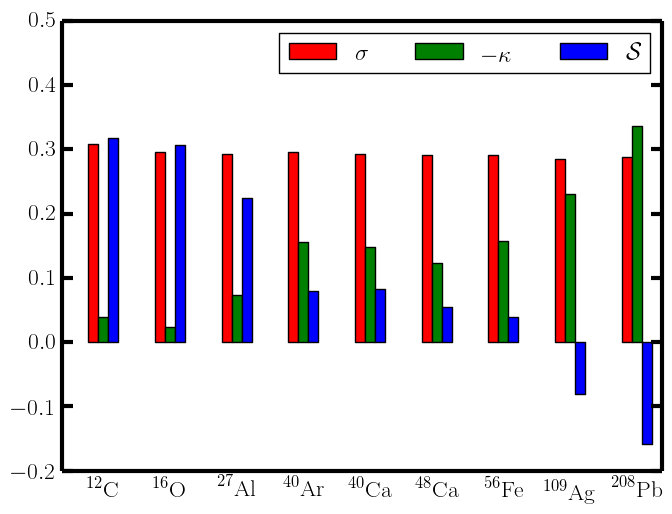
\includegraphics[scale=0.45]{./figuren/properties_ob.png}
\caption{Eigenschappen van $n^{[1]}(k)k^2$ waarbij  $n^{[1]}(k)$ \eqref{eq:ob_magnitude} berekend is met HO  \'{e}\'{e}ndeeltjes golffuncties \eqref{eq:HO_mom_radwave} met $A$-afhankelijke parameter $\omega$ gegeven door \eqref{eq:omega}. $\sigma$ wordt getoond in eenheid $fm^{-1}$. Kurtosis $\kappa$ en scheefheid $\mathcal{S}$ zijn, respectievelijk, berekend aan de hand van uitdrukkingen \eqref{eq:kurtosis} en \eqref{eq:skew}. Let op: kurtosis wordt in absolute waarde gegeven.}
\label{fig:properties}
\end{figure}
\begin{table}
\centering
\begin{tabular}{c| ccc}
$A$ & $\sigma (MeV)$ &  $\kappa$ & $\mathcal{S}$ \\
\hline
\hline
$\nuclide[12][]{C}$ & $60.82$ & $-0.04$ & $0.32$ \\
$\nuclide[16][]{O}$ & $58.36$ & $-0.02$ & $0.31$ \\
$\nuclide[27][]{Al}$ & $57.69$ & $-0.07$ & $0.23$ \\
$\nuclide[40][]{Ar}$ & $58.49$ & $-0.16$ & $0.08$ \\
$\nuclide[40][]{Ca}$ & $57.81$ & $-0.15$ & $0.08$ \\
$\nuclide[48][]{Ca}$ & $57.44$ & $-0.12$ & $0.05$ \\
$\nuclide[56][]{Fe}$ & $57.55$ & $-0.16$ & $0.04$ \\
$\nuclide[108][]{Ag}$ & $56.12$ & $-0.23$ & $-0.08$ \\
$\nuclide[208][]{Pb}$ & $56.86$ & $-0.34$ & $-0.16$ \\
\end{tabular}
\caption{Eigenschappen van $n^{[1]}(k)k^2$ waarbij  $n^{[1]}(k)$ \eqref{eq:ob_magnitude} berekend is met HO  \'{e}\'{e}ndeeltjes golffuncties \eqref{eq:HO_mom_radwave} met $A$-afhankelijke parameter $\omega$ gegeven door \eqref{eq:omega}. Kurtosis $\kappa$ en scheefheid $\mathcal{S}$ zijn, respectievelijk, berekend aan de hand van uitdrukkingen \eqref{eq:kurtosis} en \eqref{eq:skew}.}
\label{tab:properties}
\end{table} 


\newpage

\begin{figure}
\centering
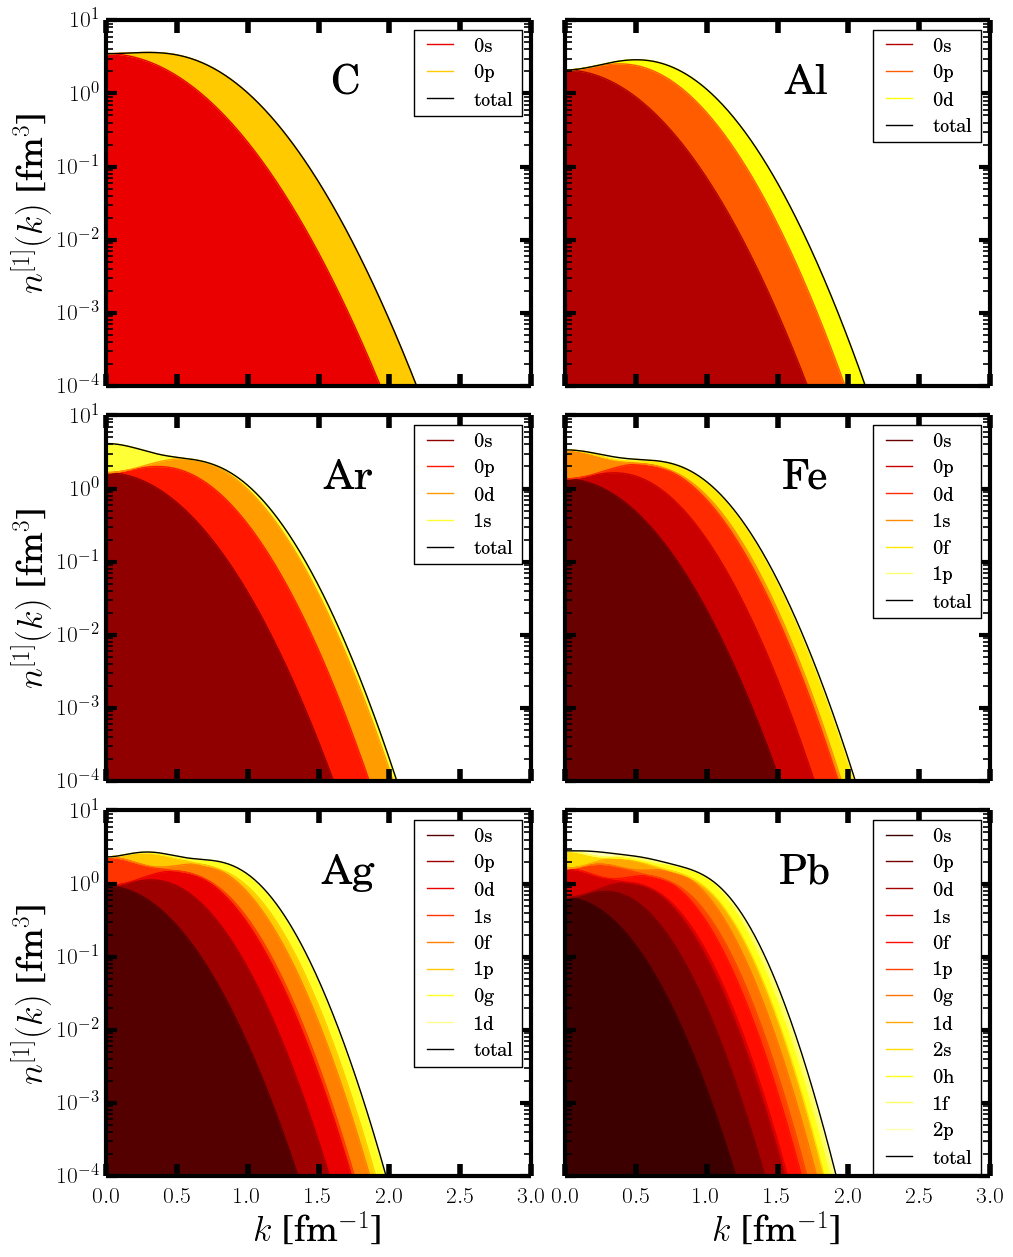
\includegraphics[scale=0.67]{./figuren/ob_multi.png}
\caption{E\'{e}ndeeltjes impulsdistributie $n^{[1]}(k)$ voor $\nuclide[12][6]{C}, \nuclide[27][13]{Al},\nuclide[40][18]{Ar},\nuclide[56][26]{Fe}, \nuclide[109][47]{Ag}, \nuclide[208][82]{Pb} $. Hier is $n^{[1]}(k)$ \eqref{eq:ob_magnitude} berekend met HO  \'{e}\'{e}ndeeltjes golffuncties \eqref{eq:HO_mom_radwave} met $A$-afhankelijke parameter $\omega$ gegeven door \eqref{eq:omega}. De normalisatie is zodanig dat $\int dk\  n^{[1]}(k)k^2 =1$.}
\label{fig:oneparticledistr}
\end{figure}

\newpage

\begin{figure}
\centering
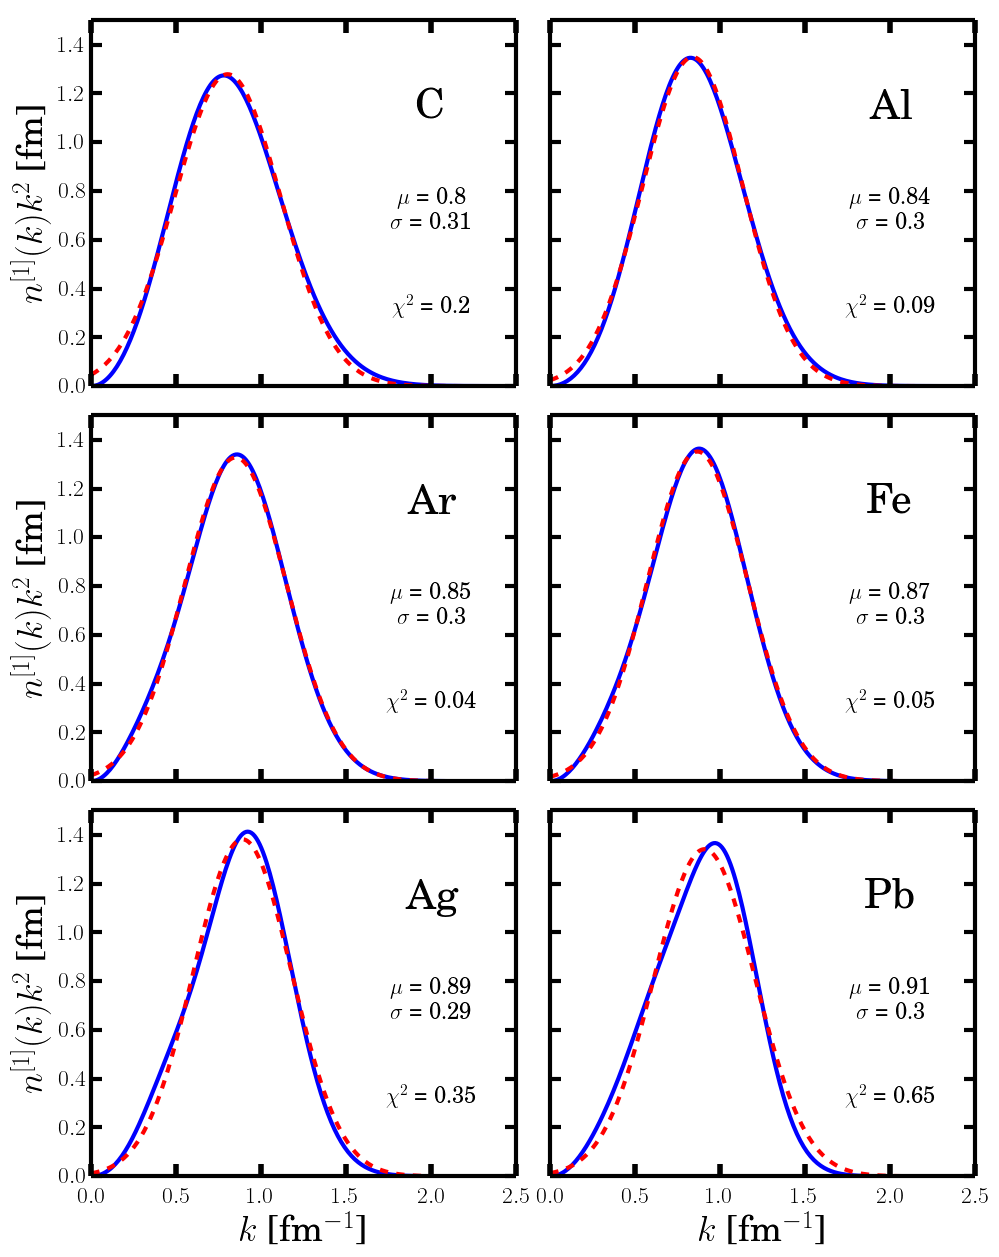
\includegraphics[scale=0.67]{./figuren/dist_normal.png}
\caption{Blauwe curve: $n^{[1]}(k)k^2$ voor $\nuclide[12][6]{C}, \nuclide[27][13]{Al},\nuclide[40][18]{Ar},\nuclide[56][26]{Fe}, \nuclide[109][47]{Ag}, \nuclide[208][82]{Pb} $. Gestreepte rode curve: een normale verdeling (\eqref{eq:gaussian}) gefit aan de resultaten. De parameters zijn $\mu$, $\sigma$ zijn gefit volgens de methode van de kleinste kwadraten en $\chi^2$ (zie \eqref{eq:chisquared}) is de goedheid van de fit. Hier is $n^{[1]}(k)$ \eqref{eq:ob_magnitude} berekend met HO  \'{e}\'{e}ndeeltjes golffuncties \eqref{eq:HO_mom_radwave} met $A$-afhankelijke parameter $\omega$ gegeven door \eqref{eq:omega}. De normalisatie is zodanig dat $\int dk\ n^{[1]}(k)k^2 =1$.}
\label{fig:oneparticledistr_2}
\end{figure}

\begin{figure}
\centering
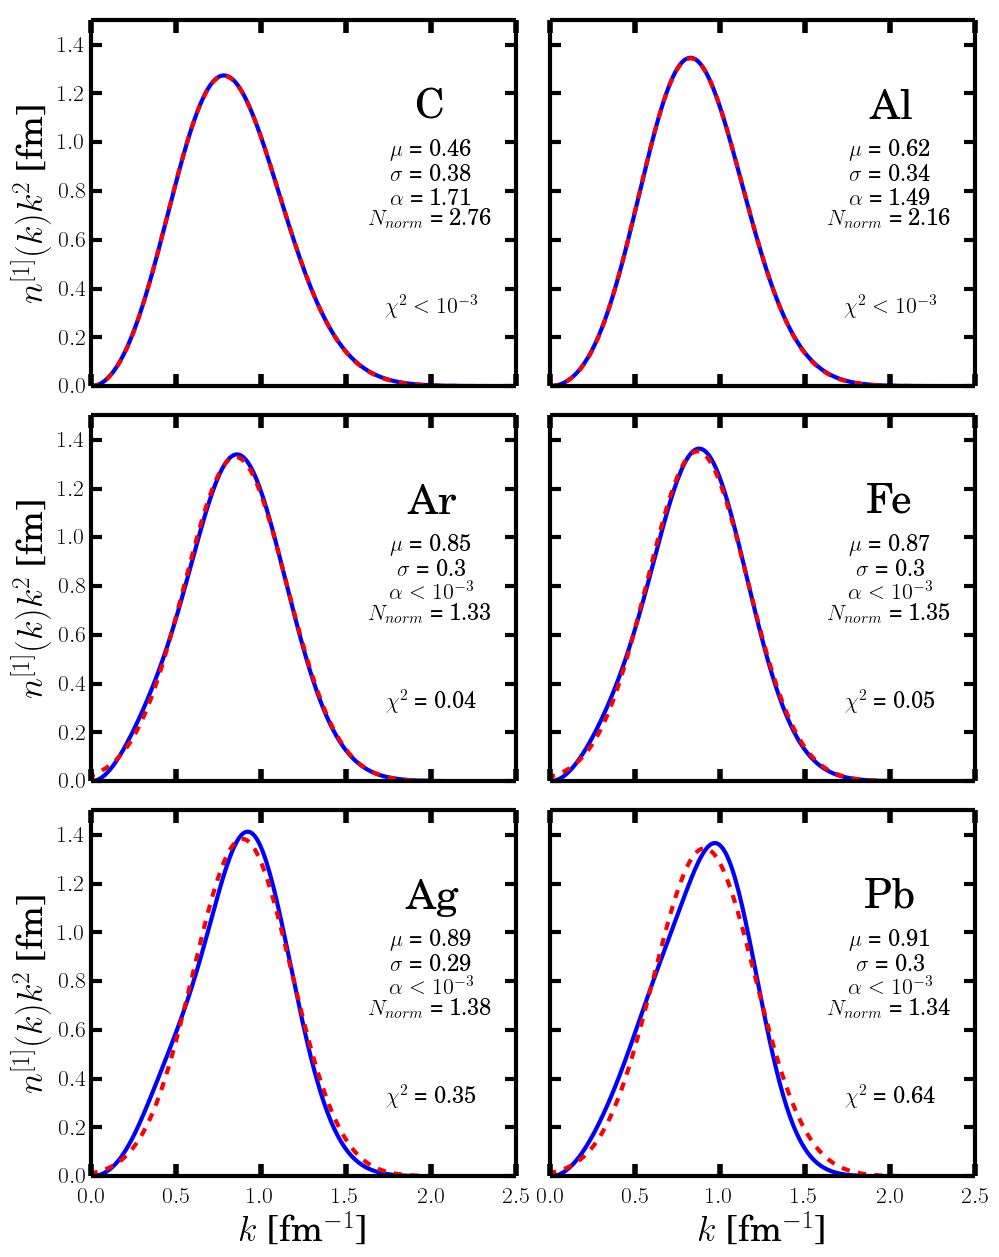
\includegraphics[scale=0.67]{./figuren/dist_powgauss.png}
\caption{Blauwe curve: $n^{[1]}(k)k^2$ voor $\nuclide[12][6]{C}, \nuclide[27][13]{Al},\nuclide[40][18]{Ar},\nuclide[56][26]{Fe}, \nuclide[109][47]{Ag}, \nuclide[208][82]{Pb} $. Gestreepte rode curve: de functie \eqref{eq:powgauss} gefit aan de resultaten volgens de methode van de kleinste kwadraten. De gefitte parameters zijn $\mu$, $\sigma$,$N_{norm}$ en $\alpha$. De parameter $\chi^2$ (zie \eqref{eq:chisquared} met $P_{normal}(k)$ vervangen door $P_{PG}(k)$, gegeven door \eqref{eq:powgauss}.) is de goedheid van de fit. Hier is $n^{[1]}(k)$ \eqref{eq:ob_magnitude} berekend met HO  \'{e}\'{e}ndeeltjes golffuncties \eqref{eq:HO_mom_radwave} met $A$-afhankelijke parameter $\omega$ gegeven door \eqref{eq:omega}. De normalisatie is zodanig dat $\int dk\  n^{[1]}(k)k^2 =1$.}
\label{fig:oneparticledistr_3}
\end{figure}


\chapter{Tweedeeltjes impulsdistributie}
\section{Algemene kenmerken}
Bij verstrooiingsexperimenten aan enkelvoudige nucleonen in een kern is er een kans dat het verstrooide nucleon initi\"{e}el deel was van een gecorreleerd paar van nucleonen. Via twee-nucleon knock-out reacties kan men tweedeeltjes impulsdistributies meten \cite{niyazov2004two} en de invloed van correlaties bestuderen. In een ODM zijn er geen correlaties tussen nucleonen. Een vergelijking met een model die correlaties bevat brengt dan de beperkingen van een ODM aan het licht.
De kans om een deeltje met impuls in het interval $[k_1,k_1+dk_1]$ te vinden wanneer een ander deeltje een impuls heeft in het interval $[k_2,k_2+dk_2]$ wordt gegeven door $ n^{[2]}(k_1,k_2)k_1^2k_2^2dk_1dk_2$ waarbij
\begin{equation}
n^{[2]}(k_1,k_2) = \int d\Omega_1 \int d\Omega_2\  n^{[2]}(\vec{k}_1,\vec{k}_2)
\end{equation}
met 
\begin{equation}
n^{[2]}(\vec{k}_1,\vec{k}_2)=\frac{1}{(2\pi)^6}\int d\vec{r}_1 \int d\vec{r}_2 \int  
    						d\vec{r}_1^{\ \prime} \int d\vec{r}_2^{\ \prime} 
    						\mathrm{e}^{i\vec{k}_1\cdot (\vec{r}_1-\vec{r}^{\ \prime}_1)} 
    						\mathrm{e}^{i\vec{k}_2\cdot(\vec{r}_2-\vec{r}^{\ \prime}_2)}
    						\rho_2(\vec{r}_1,\vec{r}_2; \vec{r}_1^{\ \prime},\vec{r}_2^{\ \prime})
\end{equation}
de tweedeeltjes impulsdistributie. Hier is

\begin{equation}
\rho_2(\vec{r}_1,\vec{r}_2, \vec{r}_1^{\ \prime},\vec{r}_2^{\ \prime}) = \int \{d\vec{r}_{3-A}\} \Psi^*_A(\vec{r}_1,\vec{r}_2,\vec{r}_3, ... ,\vec{r}_A)\Psi_A(\vec{r}_1^{\ \prime},\vec{r}_2^{\ \prime},\vec{r}_3, ... ,\vec{r}_A)
\end{equation}

de tweedeeltjes niet-diagonale dichtheidsmatrix (TNDM). Aangezien interacties tussen twee  nucleonen alleen functie zijn van de relatieve vector tussen deze twee nucleonen en de positie van hun massacentrum er niet toe doet wegens translationele invariantie van fysische wetmatigheden is het interessant de TNDM te bestuderen in functie van relatieve ($\vec{r}$) en massacentrumco\"{o}rdinaten ($\vec{R}$) (Figuur \ref{fig:coordinates}). We defini\"{e}ren deze co\"{o}rdinaten als


\begin{equation} \label{eq:rcm_def}
\vec{r}= \frac{1}{\sqrt{2}} \left(\vec{r}_1 - \vec{r}_2\right)  \qquad \vec{R}= \frac{1}{\sqrt{2}} \left(\vec{r}_1 + \vec{r}_2\right).
\end{equation}

De impulsco\"{o}rdinatendan transformeren dan als volgt,
\begin{equation} \label{eq:rcm_impusl}
\vec{k}_{12}= \frac{1}{\sqrt{2}} \left(\vec{k}_1 - \vec{k}_2\right) \qquad \vec{P}_{12}= \frac{1}{\sqrt{2}} \left(\vec{k}_1 + \vec{k}_2\right).
\end{equation}
\begin{figure}[H]
\centering
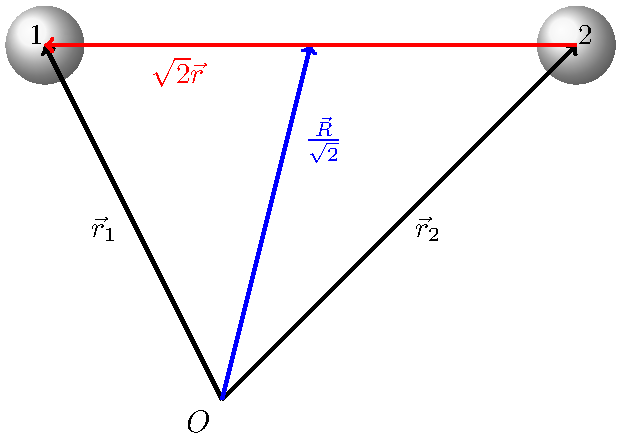
\includegraphics[scale=0.7]{./figuren/jacobi.pdf}
\caption{ Illustratie van relatieve en massacentrumco\"{o}rdinaten van twee deeltjes.}
\label{fig:coordinates}
\end{figure}
In functie van deze nieuwe co\"{o}rdinaten wordt de tweedeeltjes impulsdistributie:
\begin{equation} \label{eq:twobodydist}
n^{[2]}(\vec{k}_{12},\vec{P}_{12})=\frac{1}{(2\pi)^6}
						\int d\vec{r} \int d\vec{R} \int d\vec{r}^{\ \prime} \int d\vec{R}^{\ \prime} 
    						\mathrm{e}^{i\vec{k}_{12}\cdot (\vec{r}-\vec{r}^{\ \prime})} 
    						\mathrm{e}^{i\vec{P}_{12}\cdot(\vec{R}-\vec{R}^{\ \prime})} 
    						\rho_2(\vec{r},\vec{R}; \vec{r}^{\ \prime},\vec{R}^{\ \prime}),
\end{equation}

waarbij

\begin{equation} \label{eq:twobodydensity}
\rho_2(\vec{r},\vec{R}; \vec{r}^{\ \prime},\vec{R}^{\ \prime}) = 
							\rho_2\left(	
							\vec{r}_1=\frac{\vec{r} + \vec{R}}{\sqrt{2}},
							\vec{r}_2=\frac{-\vec{r} + \vec{R}}{\sqrt{2}},
						    \vec{r}_1^{\ \prime}=\frac{\vec{r}^{\ \prime} + \vec{R}^{\ \prime}}{\sqrt{2}},	
						    \vec{r}_2^{\ \prime}=\frac{-\vec{r}^{\ \prime} + \vec{R}^{\ \prime}}{\sqrt{2}}
						    \right).
\end{equation}

De tweedeeltjes impulsdistributie kan in het tweedekwantisatie formalisme  geschreven worden als
\begin{equation}
\label{eq:2BNDM}
n^{[2]}(\vec{k_1},\vec{k_2})= \frac{1}{A(A-1)}\bra{\Psi_A} \psi^\dagger(\vec{k}_1) \psi^\dagger(\vec{k}_2)  \psi(\vec{k}_2)  \psi(\vec{k}_1)  \ket{\Psi_A}.
\end{equation}
We verwijzen naar Appendix \ref{sec:tweede_kwant} voor de gebruikte conventies. De operator inwerkende op de grondtoestand in \eqref{eq:2BNDM} telt het aantal deeltjes met impuls $\vec{k}_1$ en $\vec{k}_2$. In de configuratieruimte wordt deze de TNDM-operator:
\begin{align} \label{eq:2BMD}
\rho(\vec{r}_1, \vec{r}_2; \vec{r}_1^{\ \prime}, \vec{r}_2^{\ \prime}) 
& = \frac{1}{A(A-1)} \braket{\Psi_A | \psi^\dagger(\vec{r}_1) \psi^\dagger(\vec{r}_2)\psi(\vec{r}^{\ \prime}_2) \psi(\vec{r}^{\ \prime}_1)|\Psi_A }.
\end{align}

De diagonaaloperator $\psi^\dagger(\vec{r}_1) \psi^\dagger(\vec{r}_2)\psi(\vec{r}_2) \psi(\vec{r}_1)$ is een teloperator die die het aantal nucleonen telt op posities $\vec{r}_1$ en  $\vec{r}_2$. De diagonaalmatrix $\rho(\vec{r}_1, \vec{r}_2; \vec{r}_1, \vec{r}_2)$ is dan een maat voor de waarschijnlijkheid om een nucleon te vinden op positie $\vec{r}_1$ op voorwaarde dat er zich een nucleon bevindt op positie $\vec{r}_2$.


\section{Het onafhankelijke-deeltjes model}


In een onafhankelijk deeltjes model waarbij de totale golffunctie van de kern een Slaterdeterminant is van \'{e}\'{e}ndeeltjesgolffuncties (\ref{eq:slater}) van bezette toestanden, wordt de TNDM (\ref{eq:twobodydensity}), rekening houdend met de orthogonaliteitsrelatie (\ref{eq:orthogonality}):

\begin{align}
\rho_2(\vec{r}_1,\vec{r}_2;\vec{r}^{\ \prime}_1,\vec{r}^{\ \prime}_2) 
&  = \frac{1}{A!} 	 \sum_{\substack{i_1 i_2 \ldots i_A}} \sum_{\substack{j_1j_2 \ldots j_A}} \varepsilon_{i_1 i_2 \ldots i_A} \varepsilon_{j_1j_2 \ldots j_A} \phi^*_{i_1}(\vec{r}_1)\phi^*_{i_2}(\vec{r}_2) \phi_{j_1}(\vec{r}_1^{\ \prime})\phi_{j_2}(\vec{r}_2^{\ \prime})
\delta_{i_3,j_3}...\delta_{i_A,j_A} \nonumber \\
& = \frac{1}{A(A-1)}\sum_{\substack{i j}} \left[\phi^*_{i}(\vec{r}_1)\phi^*_{j}(\vec{r}_2) \phi_{i}(\vec{r}_1^{\ \prime})\phi_{j}(\vec{r}_2^{\ \prime})  - \phi^*_{i}(\vec{r}_1)\phi^*_{j}(\vec{r}_2) \phi_{j}(\vec{r}_1^{\ \prime})\phi_{i}(\vec{r}_2^{\ \prime}) \right].
\end{align}
Hierbij maakten we gebruik van de volgende eigenschap van de Levi-Civita tensor:
\begin{equation}
\sum_{i_1, \ldots,  i_{A-2}} \varepsilon_{i_1 \ldots i_{A-2} jk}\ \varepsilon_{i_1 \ldots i_{A-2} mn} = (A-2)! \left( \delta_{jm}\delta_{kn} - \delta_{jn}\delta_{km} \right).
\end{equation}
Uit  \eqref{eq:1pmd} volgt dat de TNDM in een onafhankelijke-deeltjes model kan geschreven worden in functie van ENDM's:
\begin{equation}
\rho_2(\vec{r}_1,\vec{r}_2;\vec{r}^{\ \prime}_1,\vec{r}^{\ \prime}_2)  = \frac{A}{A-1} \left[\rho_1(\vec{r}_1, \vec{r}_1^{\ \prime}) \rho_1(\vec{r}_2,\vec{r}_2^{\ \prime}) - \rho_1(\vec{r}_1, \vec{r}_2^{\ \prime}) \rho_1(\vec{r}_2,\vec{r}_1^{\ \prime}) \right].
\end{equation}

Bijgevolg neemt de tweedeeltjes impulsdistributie \eqref{eq:twobodydist} in een onafhankelijk deeltjes model de volgende vereenvoudigde vorm aan:

\begin{align} \label{eq:two-body}
n^{[2]}(\vec{k}_1,\vec{k}_2) =\equiv \frac{1}{A(A-1)}\sum_{\substack{\alpha \beta}} \Braket{\alpha \beta | \vec{k}_1 \vec{k}_2}_{nas} \Braket{\vec{k}_1 \vec{k}_2 | \alpha \beta}_{nas}
\end{align}
met
\begin{equation} \label{eq:nas_twobody}
\Braket{\vec{k}_1 \vec{k}_2 | \alpha \beta}_{nas} = \frac{1}{\sqrt{2}}  \left[ \phi_{\alpha}(\vec{k}_1)\phi_{\beta}(\vec{k}_2) - \phi_{\beta}(\vec{k}_1)\phi_{\alpha}(\vec{k}_2) \right] 
\end{equation}
een totaal antisymmetrische en genormaliseerde tweedeeltjestoestand.
De sommaties in \eqref{eq:two-body} gaan over alle bezette \'{e}\'{e}ndeeltjestoestanden van de beschouwde kern.

\subsubsection{Tweedeeltjes impulsdistributies in relatieve massacentrumco\"{o}rdinaten}

De tweedeeltjes interacties $V_{ij}$ in  de volledige A-deeltjes Hamiltoniaan \eqref{eq:full_ham} zijn alleen afhankelijk van de relatieve posities van nucleonen en niet van hun positie ten opzichte van een vast punt in de ruimte. Bijgevolg wordt deze Hamiltoniaan liefst gescheiden in relatieve- en massacentrumco\"{o}rdinaten van twee deeltjes. Tweedeeltjes impulsdistributies worden dan voornamelijk bestudeerd in functie van een relatieve impuls van twee deeltjes $\vec{k}_{12}$ en de impuls van hun massacentrum $\vec{P}_{12}$. Daar we de vergelijking willen maken met distributies waarbij correlaties tussen de nucleonen in rekening worden gebracht, doen ook wij een transformatie van individuele co\"{o}rdinaten naar deze nieuwe gedefinieerd in \eqref{eq:rcm_def}. Een handige eigenschap van HO golffuncties is de orthogonale transformatie van een tweedeeltjes golffunctie naar relatieve en massacentrumco\"{o}rdinaten 
\begin{equation}
\Braket{\vec{r}_1|n_1 l_1 m_1}\braket{\vec{r}_2 | n_2 l_2 m_2} \rightarrow \braket{\vec{r}| n l m}\braket{\vec{R} | NLM}.
\end{equation}
De nieuwe golffuncties zijn nog steeds eigenfuncties van de Schr\"{o}dingervergelijking \eqref{eq:HO} aangezien de Hamiltoniaan in nieuwe co\"{o}rdinaten dezelfde gedaante heeft. We demonstreren hier voor een kern bestaande uit twee nucleonen:
\begin{equation}
\frac{1}{2M_N} (k^2_1 + k^2_2) +  \frac{1}{2} M_N \omega^2  (r^2_1 + r^2_2) =  \frac{1}{2M_N} (k_{12}^2 + P_{12}^2) +  \frac{1}{2} M_N \omega^2  (r^2 + R^2).
\end{equation} 
Deze transformatie is mogelijk door de specifieke vorm van de HO potentiaal die kwadratisch is in de positie.
In het nieuwe co\"{o}rdinatensysteem zijn ($n,\  l$) de kwantumgetallen van de relatieve beweging van de twee nucleonen  en  ($N,\ L$) beschrijven de beweging van hun massacentrum.  Men kan in beide co\"{o}rdinaatsystemen de impulsmomenten koppelen tot een totaal impulsmoment $\Lambda$:
\begin{align}
& \left| l_1-l_2 \right| \leq \Lambda \leq l_1 + l_2 \\
& \left| l-L \right| \leq \Lambda \leq l+ L
\end{align}

Twee deeltjes in een gekoppelde toestand hebben een welbepaald impulsmoment $\Lambda$ en projectie $M_\Lambda$  en deze toestand kan geschreven worden als:
\begin{align}
\Ket{n_1l_1n_2l_2;\Lambda M_\Lambda} = \sum_{m_1, m_2} \Ket{n_1l_1m_1n_2l_2m_2} \Braket{l_1m_1,l_2m_2| \Lambda M_\Lambda} 
\end{align}
En ook in het nieuwe co\"{o}rdinatensysteem kunnen we de impulsmomenten koppelen:
\begin{align}
\Ket{nlNL;\Lambda M_\Lambda} = \sum_{m, M} \Ket{nlm NLM} \Braket{lm LM|\Lambda M_\Lambda}.
\end{align}
Een HO tweedeeltjes golffunctie met totaal impulsmoment $\Lambda$  en projectie $M_\Lambda$ heeft een orthogonale transformatie van individuele co\"{o}rdinaten naar relatieve en massacentrumco\"{o}rdinaten, namelijk de Moshinsky-transformatie \cite{moshinsky1959transformation}:
\begin{align} \label{eq:moshinsky_trans}
\Ket{n_1l_1n_2l_2;\Lambda M_\Lambda} = \sum_{nl, N\Lambda} \Ket{nlNL;\Lambda M_\Lambda} \Braket{nlNL;\Lambda | n_1l_1n_2l_2;\Lambda}_{MB}.
\end{align}
De transformatico\"{e}ffici\"{e}nten $\Braket{nlNL;\Lambda | n_1l_1n_2l_2;\Lambda}$ zijn gekend als de Moshinsky-co\"{e}ffici\"{e}nten en zijn onafhankelijk van $M_\Lambda$. De energie van een deeltje ($E$), neem nu bijvoorbeeld een zeker deeltje "1",  in een HO potentiaal is $\hbar\omega  (2n_1+l_1+ \frac{3}{2})$. Daar de totale energie van twee deeltjes dezelfde moet zijn in verschillende co\"{o}rdinaatsystemen moet er gelden dat
\begin{equation}
2n_1 + l_1 + 2n_2 + l_2 = 2n + l + 2N + L.
\end{equation}
De Moshinskyco\"{e}ffici\"{e}nten zijn nul als deze gelijkheid niet is voldaan. Een recursieve methode voor de berekening van deze co\"{e}ffici\"{e}nten kan gevonden worden in Appendix \ref{sec:recursif_mosh}.


\subsubsection{Tweedeeltjes impulsdistributie voor harmonische oscillator potentiaal}
Daar we de tweedeeltjes impulsdistributie \eqref{eq:two-body} willen bestuderen in functie van relatieve impuls en massacentrumimpuls moeten de geantisymmetriseerde toestanden \eqref{eq:nas_twobody} geschreven worden in functie van $\vec{k}_{12}$ en $\vec{P}_{12}$. De ontwikkeling van \eqref{eq:nas_twobody} in toestanden die functie zijn van $\vec{k}_{12}$ en $\vec{P}_{12}$  kan men vinden in Appendix \ref{sec:antisym}:
\begin{equation}
\Braket{\vec{k}_1 \vec{k}_2 | \alpha \beta}_{nas} = \sum_{\substack{nlm_l \\ NLM_L}} \sum_{S M_S}   \sum_{T M_T}  C_{\alpha \beta}^{ nlm_l NLM_L  S M_S T M_T} \Ket{ nlm_l(\vec{k}_{12})  NLM_L(\vec{P}_{12}) S M_S  T M_T}.
\end{equation}

Met behulp van deze transformatie wordt de tweedeeltjes impulsdistributie in functie van relatieve- en massacentrumimpuls \eqref{eq:two-body} gevonden:
\begin{align} \label{eq:2BMD_uitgewerkt}
n^{[2]}(\vec{k}_{12},\vec{P}_{12}) & =\frac{1}{A(A-1)}\sum_{\substack{\alpha \beta \\ \alpha  \neq \beta}} \sum_{\substack{nlm_l \\ NLM_L}} \sum_{\substack{n^{\prime}l^{\prime}m^{\prime}_l \\ N^{\prime}L^{\prime}M^{\prime}_L}} \sum_{S M_S} \sum_{T M_T}  \left(C_{\alpha \beta}^{ nlm_l NLM_L  S M_S T M_T} \right)^\dagger  C_{\alpha \beta}^{ n^{\prime} l^{\prime} m^{\prime}_l N^{\prime} L^{\prime} M^{\prime}_L  S M_S T M_T} \nonumber
\\ & \phantom{{a}=1}\times \psi^*_{nlm_l}(\vec{k}_{12}) \psi^*_{NLM_L}(\vec{P}_{12}) \psi_{n^{\prime}l^{\prime}m^{\prime}_l}(\vec{k}_{12}) \psi_{N^{\prime}L^{\prime}M^{\prime}_L}(\vec{P}_{12})
\end{align}
waarbij $\psi$ de HO golffunctie \eqref{eq:splits_momentum} is. De golffunctie is kern-afhankelijk door parameter $\omega$, gegeven door \eqref{eq:omega}.

\section{Resultaten}

Allereerst bestuderen we de relatieve tweedeeltjes impulsdistributie die we krijgen door  \eqref{eq:2BMD_uitgewerkt} te integreren over de massacentrumimpuls $\vec{P}$ en over alle directionele afhankelijkheid:
\begin{align} \label{eq:rel_two}
n^{[2]}(k_{12}) & = \int d\Omega_{k_{12}}\int d\vec{P}_{12}\ n^{[2]}(\vec{k}_{12},\vec{P}_{12}) \nonumber \\
							& = \sum_{l} n_2^{l}(k_{12})
\end{align}
waarbij
\begin{align*}
n_2^{l}(k_{12}) = \frac{1}{A(A-1)} \sum_{\substack{\alpha \beta}} \sum_{\substack{nm_l \\ NLM_L}} \sum_{\substack{n^{\prime} }} \sum_{\substack{S M_S \\T M_T}} &  \left( C_{\alpha \beta}^{nlm_l NLM_L  S M_S T M_T} \right)^\dagger  C_{\alpha \beta}^{ n^{\prime} lm_l NLM_L  S M_S T M_T} \\ \ \times & K_{nl}(k_{12}) K_{n^{\prime} l}(k_{12}).
\end{align*}
Hier is $K_{nl}(k)$ de radi\"{e}le HO golffunctie in de impulsruimte gedefinieerd in vergelijking \eqref{eq:HO_mom_radwave}.
Resultaten worden getoond in Figuur \ref{fig:twoparticledistr_rel_log} waarbij we $n^{[2]}(k_{12})$ op een logaritmische schaal tonen omdat uit onderzoek waarbij kortedracht correlaties in rekening worden gebracht (\cite{maarten,wiringa2014nucleon}), blijkt dat correlaties zorgen voor een brede staart in de distributie vanaf $k_{12} \gtrsim 1.5\ fm^{-1}$. Een zichtbaar verschil toont zich alleen op een logaritmische schaal.  Resultaten uit GV berekeningen zijn dus relevant tot ongeveer $1.5\ fm^{-1}$. De distributie $n^{[2]}(k_{12})k_{12}^2dk_{12}$ geeft de kans om twee nucleonen te vinden met een onderling relatieve impuls in het interval $[ k_{12}, k_{12}+ d k_{12} ]$ en is afgebeeld in Figuur \ref{fig:twoparticledistr_rel} voor verschillende kernen. De bijdragen van relatieve impulsmoment $l$ worden getoond ter vergelijking met een model met correlaties zodat men kan zien welke $l$ het meest worden be\"{i}nvloed door deze correlaties. Dat interacties tussen nucleonen de bezettingen van de relatieve $l$ be\"{i}nvloeden is int\"{i}utief te begrijpen als men kijkt naar overlap van twee nucleonen in verschillende relatieve $l$ toestanden. Bij $l=0$ is de overlap het grootst en we verwachten dat de bezetting van deze toestand het meest zal veranderen bij het invoeren van correlaties. Uit de resultaten valt ook op dat twee nucleonen zich voornamelijk in een $l=1$ toestand bevinden. Afwijkingen van een normale distributie, gekarakteriseerd door kurtosis $\kappa$ en scheefheid $\mathcal{S}$ zijn duidelijk afhankelijk van de massa $A$ van de kern zoals weergegeven in Figuur \ref{fig:properties_rel}. Net zoals bij de \'{e}\'{e}ndeeltjes impulsdistributie groeit ook bij de tweedeeltjes impulsdistributies de absolute waarde van de kurtosis met toenemende $A$. Kurtosis is steeds negatief zodat de distributies kleinere staarten en een bredere piek hebben ten opzichte van een normale distributie. 
De andere parameter die afwijking van de normale distributie karakteriseert, scheefheid, neemt af naarmate $A$ groter wordt en is steeds positief, de distributies zijn dus rechts scheef. 
Ook valt op dat de spreiding rond het gemiddelde ruwweg onafhankelijk is van de massa van de kern. Daar de afwijkingen steeds klein zijn kunnen we besluiten dat de relatieve tweedeetjesimpuls bij benadering normaal verdeeld is voor de verschillende kernen.

Vervolgens bestuderen we de impulsdistributie van het massacentrum van twee deeltjes gegeven door 
\begin{align} \label{eq:cm_two}
n^{[2]}(P_{12}) & = \int d\Omega_{P_{12}}\int d\vec{k}_{12}\ n^{[2]}(\vec{k}_{12},\vec{P}_{12}) \nonumber \\
				 & = \sum_{l}  n_2^{l}(P_{12})
\end{align}
waarbij
\begin{align*} 
n_2^{l}(P_{12}) = \frac{1}{A(A-1)} \sum_{\substack{\alpha \beta }} \sum_{\substack{nm_l \\ NLM_L}} \sum_{N^{\prime}} \sum_{\substack{S M_S \\T M_T}} &  \left( C_{\alpha \beta}^{nlm_l NLM_L  S M_S T M_T} \right)^\dagger  C_{\alpha \beta}^{ n lm_l N^{\prime}LM_L  S M_S T M_T} \\ \ \times & K_{NL}(P_{12}) K_{N^{\prime} L}(P_{12}). 
\end{align*}
Hier is $K_{NL}(P_{12})$ de radi\"{e}le HO golffunctie in de impulsruimte gedefinieerd in vergelijking \eqref{eq:HO_mom_radwave}.
Resultaten zijn afgebeeld in Figuur \ref{fig:twoparticledistr_cm}. De kans om twee nucleonen te vinden waarvan het massacentrum een impuls heeft in het interval $[ P_{12}, P_{12}+ dP_{12} ]$ wordt gegeven door $n^{[2]}(P_{12})P_{12}^2dP_{12}$. De afwijkingen van een normale distributie vertonen dezelfde karakteristieken als bij de relatieve impulsdistributie. De kurtosis van de berekende distributies is steeds negatief en de absolute waarde wordt steeds groter met toenemende massa $A$ van de kern. De scheefheid neemt af met de massa. De breedte van de massacentrum impulsdistributies is onafhankelijk van de massa van de kern. De scheefheid en kurtosis zijn steeds klein dus wordt de impuls van het tweedeeltjes massacentrum relatief goed beschreven door een normale verdeling.
Contributies van relatieve orbitaal kwantumgetal $l$ zijn weergegeven ter vergelijking met een model met correlaties. Ook hier gelden dezelfde conclusies als bij de relatieve distributie in verband met de bijdragen van de verschillende $l$, namelijk $l=0$ zal het meest be\"{i}vloed worden door correlaties tussen de nucleonen. 
In Figuur \ref{fig:vergelijking} vergelijken we onze resultaten van de relatieve en massacentrum impulsdistributies met overeenkomstige GV resultaten van M. Vanhalst \cite{maarten}. Onze resultaten stemmen overeen.

Tenslotte bestuderen we de tweedeeltjes impulsdistributie in functie van de hoek $\theta_{kP}$ tussen $\vec{k}_{12}$ en  $\vec{P}_{12}$:
\begin{align} \label{eq:angle_tb2}
n^{[2]}(\theta_{kP}) & = 8\pi^2 \int dP_{12} \int dk_{12}\  P_{12}^2\ k_{12}^2\ n^{[2]}(\vec{k}_{12},\vec{P}_{12}) \nonumber \\
& =   \frac{8\pi^2}{A(A-1)} \sum_{\substack{\alpha \beta }} \sum_{\substack{nlm_l \\ NLM_L}} \sum_{\substack{m_l^{\prime} \\\ M_L^{\prime} }} \sum_{\substack{S M_S \\T M_T}}  \left( C_{\alpha \beta}^{nlm_l NLM_L  S M_S T M_T} \right)^\dagger  C_{\alpha \beta}^{ n lm_l^{\prime} NLM_L^{\prime}  S M_S T M_T} \nonumber \\ & \times  \ Y^*_{l m_l}(0,0) Y_{l m_l^{\prime}}(0,0) Y^*_{L M_L}(\theta_{kP},0)  Y_{L M_L^{\prime}}(\theta_{kP},0). 
\end{align}
Hierbij is overgegaan naar een assenstelsel weergegeven in Figuur \ref{fig:assen}.
\begin{figure}[h]
\centering
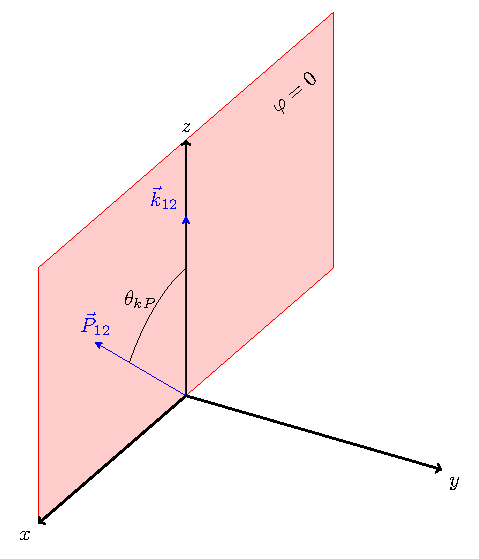
\includegraphics[scale=0.85]{./figuren/assenstelsel1.pdf}
\caption{We kunnen een transformatie doen naar dit co\"{o}rdinatensysteem zodat alle hoeken verdwijnen behalve de hoek tussen $\vec{k}_{12}$ en $\vec{P}_{12}$: de azumitale hoek $\varphi$ is voor beide vectoren nul en ook de poolhoek van $\vec{k}_{12}$, genaamd $\theta_{k_{12}}$, is nul.  }
\label{fig:assen}
\end{figure}

Resultaten worden getoond in Figuur \ref{fig:angle}. Voor alle kernen zijn deze maximaal bij $\theta_{kP} = \pi/2$. Als $\vec{k}_{12}$ en $\vec{P}_{12}$ loodrecht staan op elkaar dan volgt uit hun  definities \eqref{eq:rcm_impusl} dat de groottes van de individuele impulsen van de deeltjes even groot zijn ($|\vec{k}_1| = |\vec{k}_2|$). De kans om twee nucleonen te vinden waarvan de relatieve impuls een hoek $\theta_{kP}$ vormt met de impuls van hun massacentrum wordt gegeven door $n^{[2]}(\theta_{kP})\sin{\theta_{kP}}d\theta_{kP}$. Daar $\sin{\theta_{kP}}$ ook piekt bij $\theta_{kP} = \pi/2$ is deze distributie voor alle kernen maximaal bij een loodrechte configuratie van $\vec{k}_{12}$ en $\vec{P}_{12}$. Dus twee nucleonen bevinden zich bij voorkeur in een toestand waarbij ze een even grote impuls hebben. Dit is niet alleen het gevolg van de factor $\sin{\theta_{kP}}$ afkomstig van de faseruimte, maar ook van de distributie $n^{[2]}(\theta_{kP})$ zelf.  We hebben ook een Monte-Carlosimulatie gedaan met $10^6$ evenementen. Bij elk evenement genereren we twee \'{e}\'{e}ndeeltjes impulsen waarbij de grootte van deze impulsen ($|\vec{k}_1|$ en $|\vec{k}_2|$) worden getrokken uit de berekende \'{e}\'{e}ndeeltjes impulsdistributies, getoond in Figuren \ref{fig:oneparticledistr_2} en \ref{fig:oneparticledistr_3}. De hoeken van deze \'{e}\'{e}ndeeltjes impulsen zijn gegenereerd uit een uniforme verdeling op een eenheidssfeer. Uit deze twee impulsen berekenen we dan de relatieve impuls en de impuls van het massacentrum aan de hand van definities \eqref{eq:rcm_impusl}. De hoek tussen $\vec{k}_{12}$ en $\vec{P}_{12}$ bepalen we via
\begin{equation} \label{eq:thetakp}
\cos{\theta_{kP}} = \frac{\vec{P}_{12} \cdot \vec{k}_{12}}{|\vec{P}_{12}| |\vec{k}_{12}|}.
\end{equation}
In Figuur \ref{fig:mc} is het resultaat van deze simulatie weergegeven voor koolstof. Het resultaat sluit aan bij de theoretische verdeling uit Figuur \ref{fig:angle}.
\begin{figure}
\centering
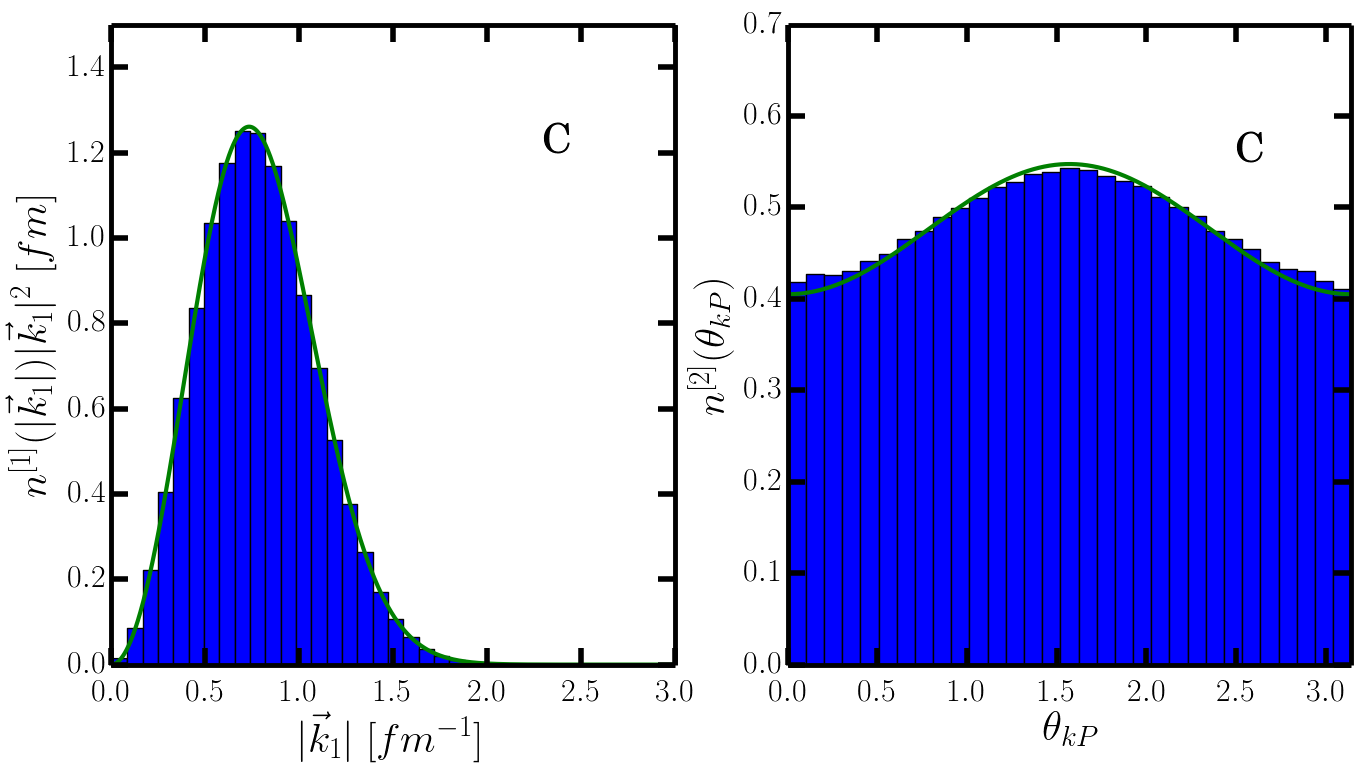
\includegraphics[scale=0.35]{./figuren/carbon.png}
\caption{De resultaten van een Monte-Carlosimulatie met $10^6$ evenementen. Links: \'{e}\'{e}ndeeltjes impuls gegenereerd volgens de \'{e}\'{e}ndeeltjes impulsdistributie van $\nuclide[12][6]{C}$ berekend in Hoofstuk \ref{eendeeltjes} (Zie Figuren \ref{fig:oneparticledistr_2} en \ref{fig:oneparticledistr_3}, hier weergegeven met een groene curve). Rechts: de verdeling van de hoek $\theta_{kP}$ tussen $\vec{k}_{12}$ en $\vec{P}_{12}$ , gegeven door uitdrukking \eqref{eq:thetakp}. De groene curve stelt de theoretische verdeling voor uit Figuur \ref{fig:angle}.}
\label{fig:mc}
\end{figure}
Als we de eigenschappen van de hoekdistributies bekijken valt op dat de scheefheid steeds nul is, met andere woorden de distributies zijn steeds symmetrisch rond $\theta_{kP} = \pi/2$. De kurtosis en  de variantie vari\"{e}ren weinig van kern tot kern. De eerstgenoemde is steeds negatief en groter in absolute waarde dan bij de vorige tweedeeltjes impulsdistributies.

\begin{figure}[H]
\centering
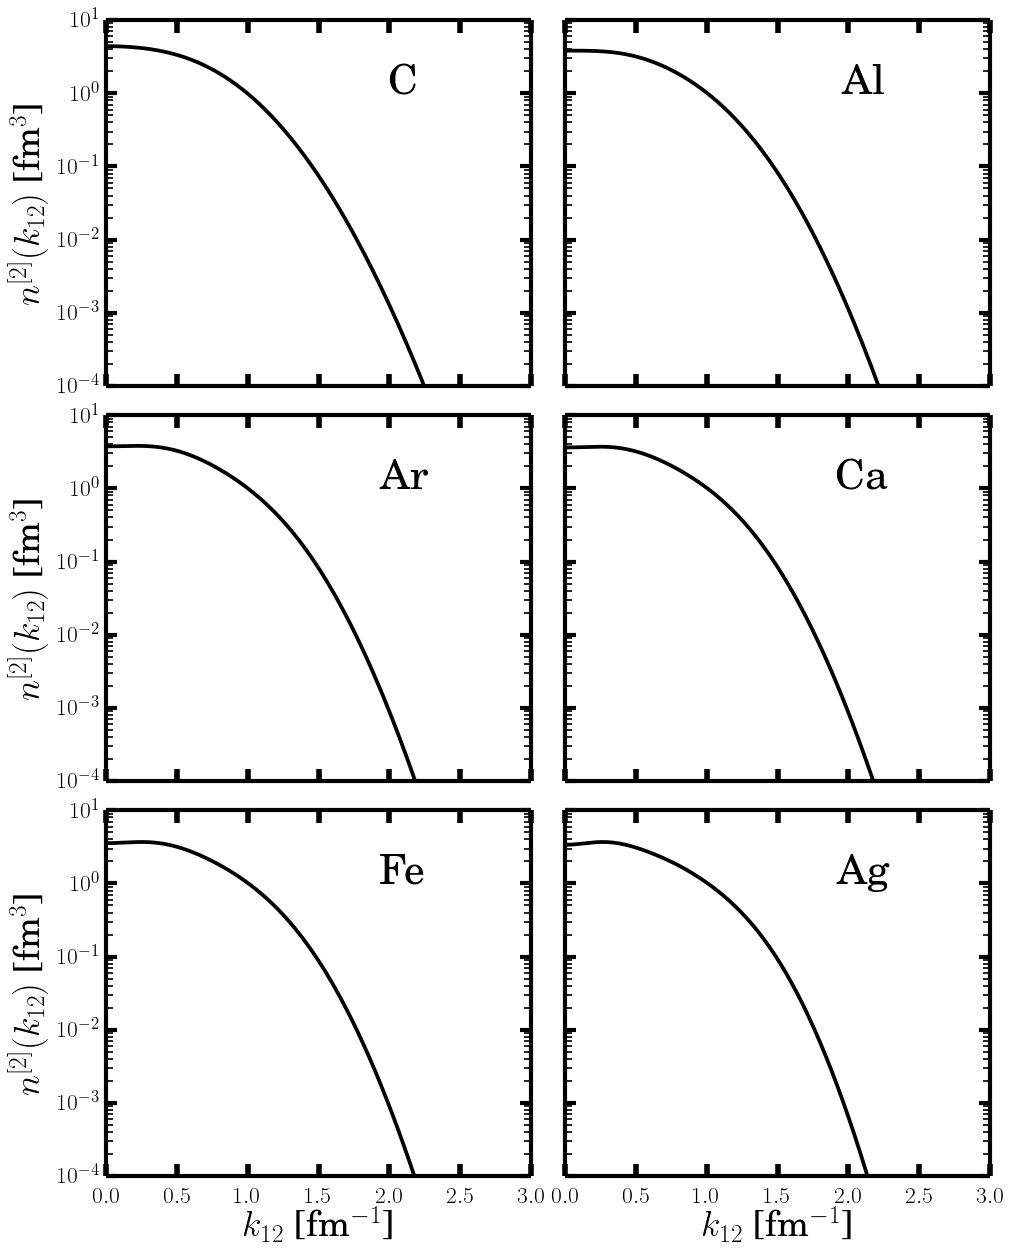
\includegraphics[scale=0.65]{./figuren/multi_rel_log.png}
\caption{Berekende $n^{[2]}(k_{12})$ gegeven door uitdrukking \eqref{eq:rel_two} voor $ \nuclide[12][6]{C}, \nuclide[27][13]{Al},\nuclide[40][18]{Ar},\nuclide[48][20]{Ca},\nuclide[56][26]{Fe},\nuclide[109][47]{Ag}$. De normalisatie is zodanig dat $\int dk_{12}\ k_{12}^2\ n^{[2]}(k_{12}) = 1$. }
\label{fig:twoparticledistr_rel_log}
\end{figure}

\begin{figure}[H]
\centering
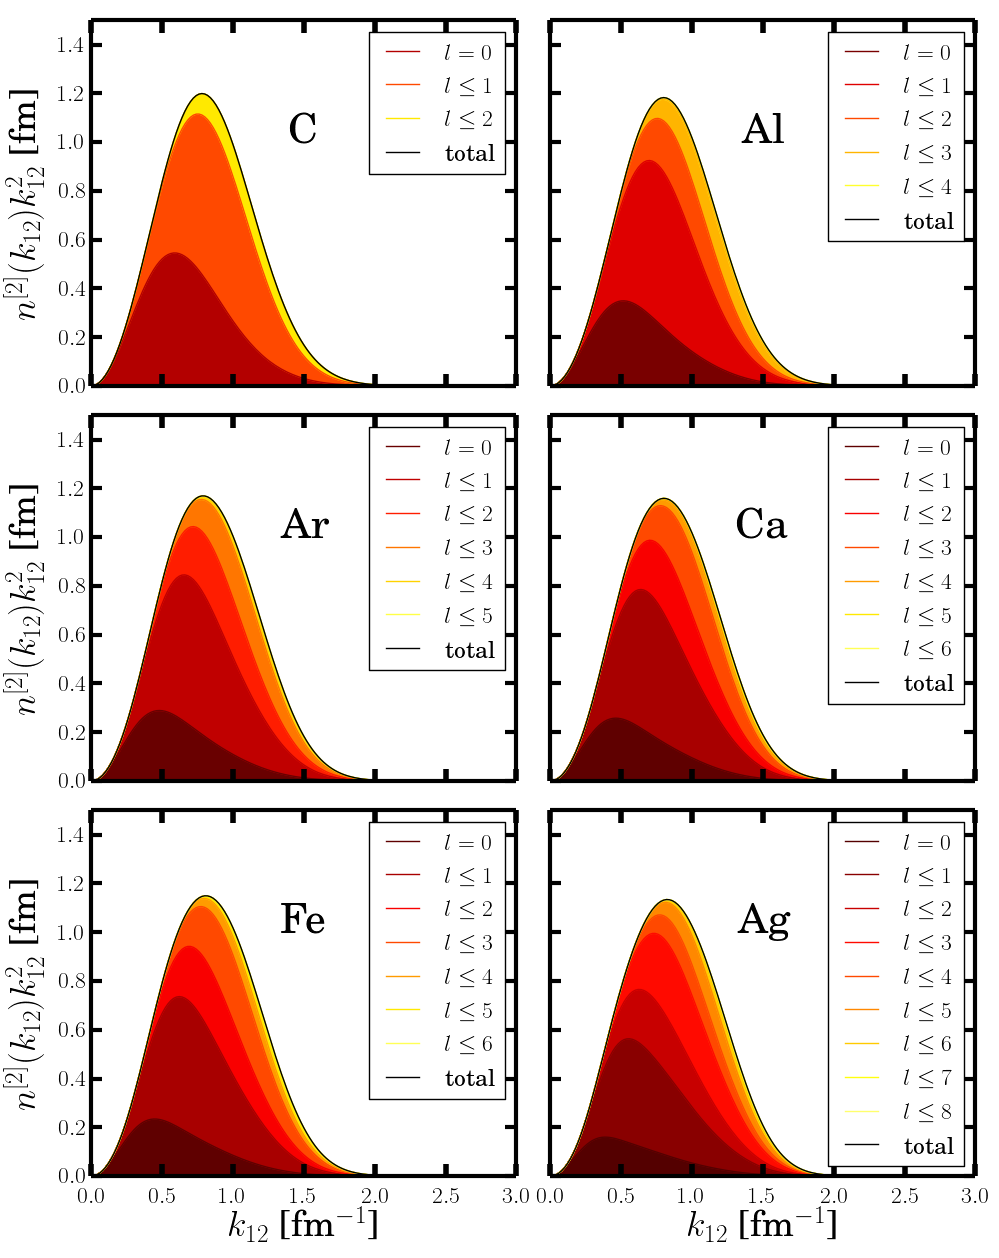
\includegraphics[scale=0.65]{./figuren/multi_rel.png}
\caption{Berekende $n^{[2]}(_{12})k_{12}^2$, waarbij $n^{[2]}(k_{12})$ gegeven door uitdrukking \eqref{eq:rel_two}, voor $ \nuclide[12][6]{C}, \nuclide[27][13]{Al},\nuclide[40][18]{Ar},\nuclide[48][20]{Ca},\nuclide[56][26]{Fe},\nuclide[109][47]{Ag}$. De normalisatie is zodanig dat $\int dk_{12}\ k_{12}^2\ n^{[2]}(k_{12}) = 1$. De bijdragen van de tweedeeltjes relatieve impulsmomenten $l$ worden getoond. }
\label{fig:twoparticledistr_rel}
\end{figure}


\begin{figure}[H]
\centering
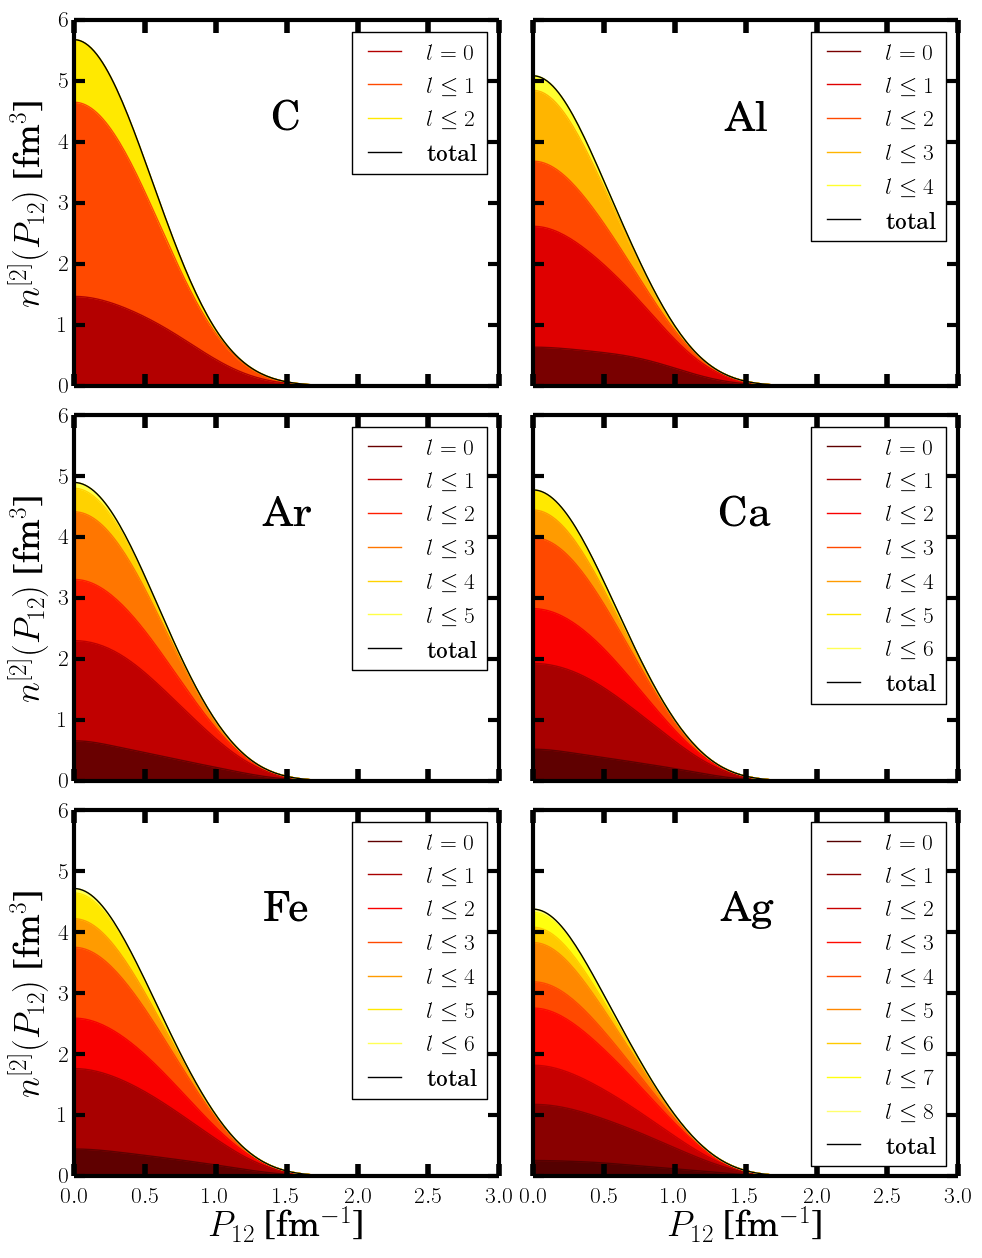
\includegraphics[scale=0.65]{./figuren/multi_cm.png}
\caption{$n^{[2]}(P_{12})$ gegeven door uitdrukking \eqref{eq:cm_two} voor $ \nuclide[12][6]{C}, \nuclide[27][13]{Al},\nuclide[40][18]{Ar},\nuclide[48][20]{Ca},\nuclide[56][26]{Fe},\nuclide[109][47]{Ag}$. Normalisatie is zodanig dat $\int dP_{12}\ P_{12}^2\ n^{[2]}(P_{12}) = 1$. De bijdragen van de tweedeeltjes relatieve impulsmomenten $l$ worden  getoond.}
\label{fig:twoparticledistr_cm}
\end{figure}

\begin{figure}[H]
\centering
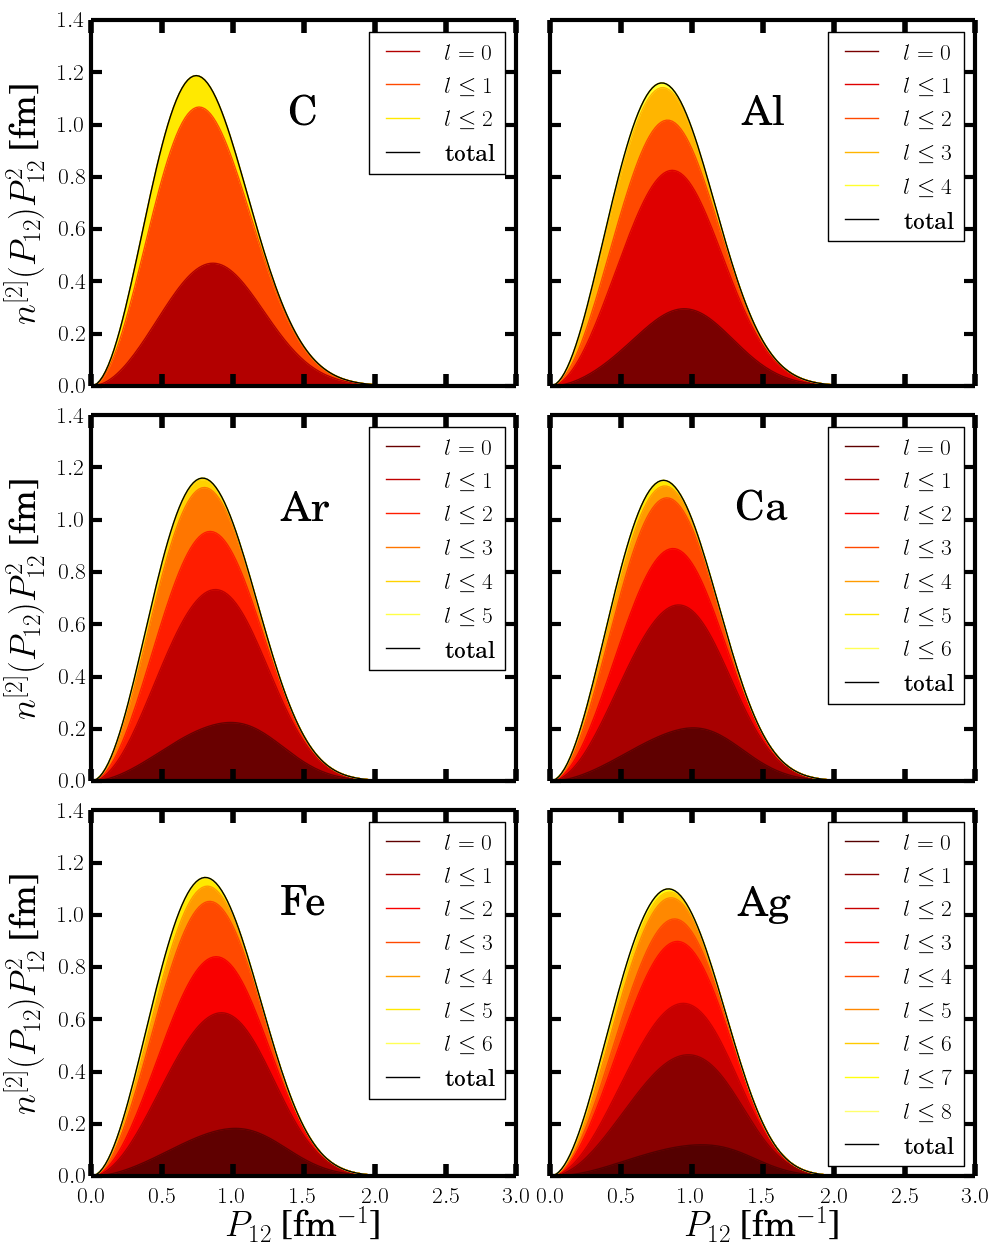
\includegraphics[scale=0.65]{./figuren/multi_cm_prob.png}
\caption{$n^{[2]}(P_{12})P_{12}^2$, met $n^{[2]}(P_{12})$ gegeven door uitdrukking \eqref{eq:cm_two}, voor $ \nuclide[12][6]{C}, \nuclide[27][13]{Al},\nuclide[40][18]{Ar},\nuclide[48][20]{Ca},\nuclide[56][26]{Fe},\nuclide[109][47]{Ag}$. De normalisatie is zodanig dat $\int dP_{12}\ P_{12}^2\ n^{[2]}(P_{12}) = 1$. De bijdragen van de tweedeeltjes relatieve impulsmomenten $l$ worden getoond.}
\label{fig:twoparticledistr_cm_prob}
\end{figure}


\begin{table}
\centering
\begin{tabular}{c| ccc}
$A$ & $\sigma (MeV)$ &  $\kappa$ & $\mathcal{S}$ \\
\hline
\hline
$\nuclide[12][]{C}$ & $63.924$ & $-0.086$ & $0.329$ \\
$\nuclide[27][]{Al}$ & $64.043$ & $-0.177$ & $0.283$ \\
$\nuclide[40][]{Ar}$ & $63.959$ & $-0.235$ & $0.275$ \\
$\nuclide[48][]{Ca}$ & $64.076$ & $-0.264$ & $0.254$ \\
$\nuclide[56][]{Fe}$ & $64.461$ & $-0.279$ & $0.250$ \\
$\nuclide[108][]{Ag}$ & $64.658$ & $-0.364$ & $0.206$ \\
\end{tabular}
\caption{De breedte $\sigma$, de kurtosis $\kappa$ en de scheefheid $\mathcal{S}$ van relatieve tweedeeltjes impulsdistributies van Figuur \ref{fig:twoparticledistr_rel}.}
\label{tab:properties_rel}
\end{table}

\begin{figure}
\centering
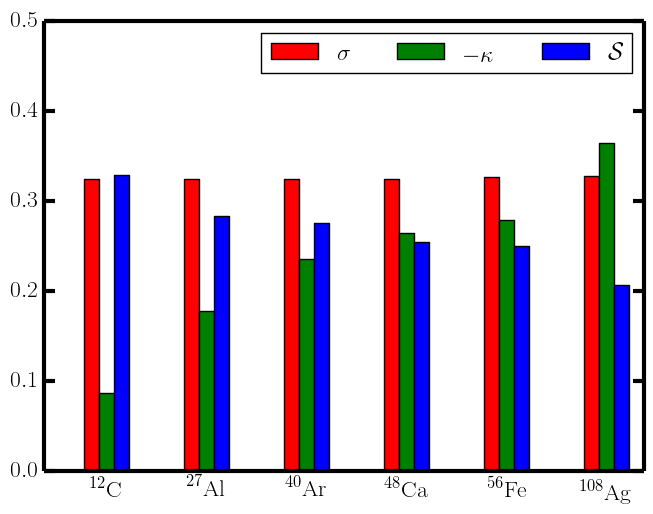
\includegraphics[scale=0.45]{./figuren/properties_rel.png}
\caption{De breedte $\sigma$, de kurtosis $\kappa$ en de scheefheid $\mathcal{S}$ van relatieve tweedeeltjes impulsdistributies van Figuur \ref{fig:twoparticledistr_rel}. Numerieke waarden staan in Tabel \ref{tab:properties_rel}. De kurtosis is steeds negatief en wordt in absolute waarde getoond.}
\label{fig:properties_rel}
\end{figure}

\begin{figure}
\centering
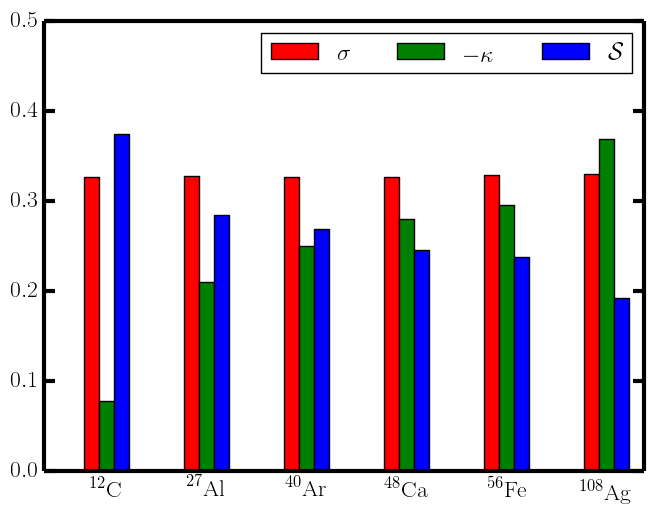
\includegraphics[scale=0.45]{./figuren/properties_cm.png}
\caption{De breedte $\sigma$, de kurtosis $\kappa$ en de scheefheid $\mathcal{S}$ van massacentrum tweedeeltjes impulsdistributies van Figuur \ref{fig:twoparticledistr_cm_prob}. Numerieke waarden staan in Tabel \ref{tab:properties_cm}. De kurtosis is steeds negatief en wordt in absolute waarde getoond.}
\label{fig:properties_cm}
\end{figure}

\begin{figure}
\centering
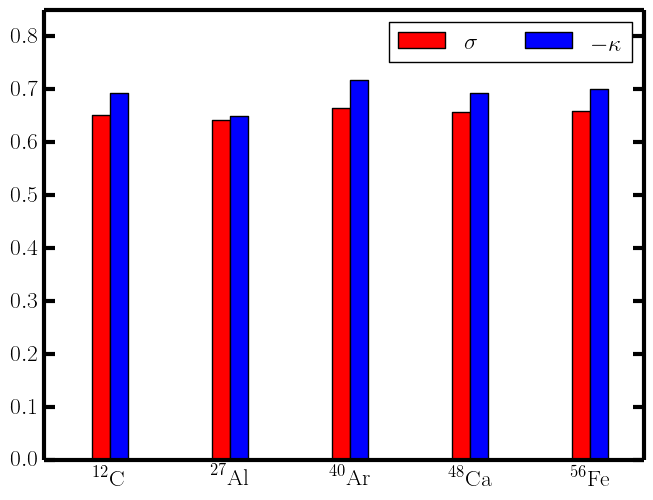
\includegraphics[scale=0.45]{./figuren/properties_angle.png}
\caption{De breedte $\sigma$ en de kurtosis $\kappa$ van de hoekdistributies tweedeeltjes impuls van Figuur \ref{fig:angle}. Scheefheid van deze distributie $\mathcal{S}$ is nul voor alle beschouwde kernen. De kurtosis is steeds negatief en wordt in absolute waarde getoond.}
\label{fig:properties_angle}
\end{figure}

\begin{table}
\centering
\begin{tabular}{c| ccc}
$A$ & $\sigma (MeV)$ &  $\kappa$ & $\mathcal{S}$ \\
\hline
\hline
$\nuclide[12][]{C}$ & $64.309$ & $-0.077$ & $0.374$ \\
$\nuclide[27][]{Al}$ & $64.653$ & $-0.210$ & $0.284$ \\
$\nuclide[40][]{Ar}$ & $64.353$ & $-0.250$ & $0.269$ \\
$\nuclide[48][]{Ca}$ & $64.509$ & $-0.280$ & $0.245$ \\
$\nuclide[56][]{Fe}$ & $64.866$ & $-0.295$ & $0.237$ \\
$\nuclide[108][]{Ag}$ &$64.962$&	$-0.369$&	$0.192$ \\
\end{tabular}
\caption{De breedte $\sigma$, de kurtosis $\kappa$ en de scheefheid $\mathcal{S}$ van massacentrum tweedeeltjes impulsdistributies van Figuur \ref{fig:twoparticledistr_cm_prob}.}
\label{tab:properties_cm}
\end{table}

\begin{figure}
\centering
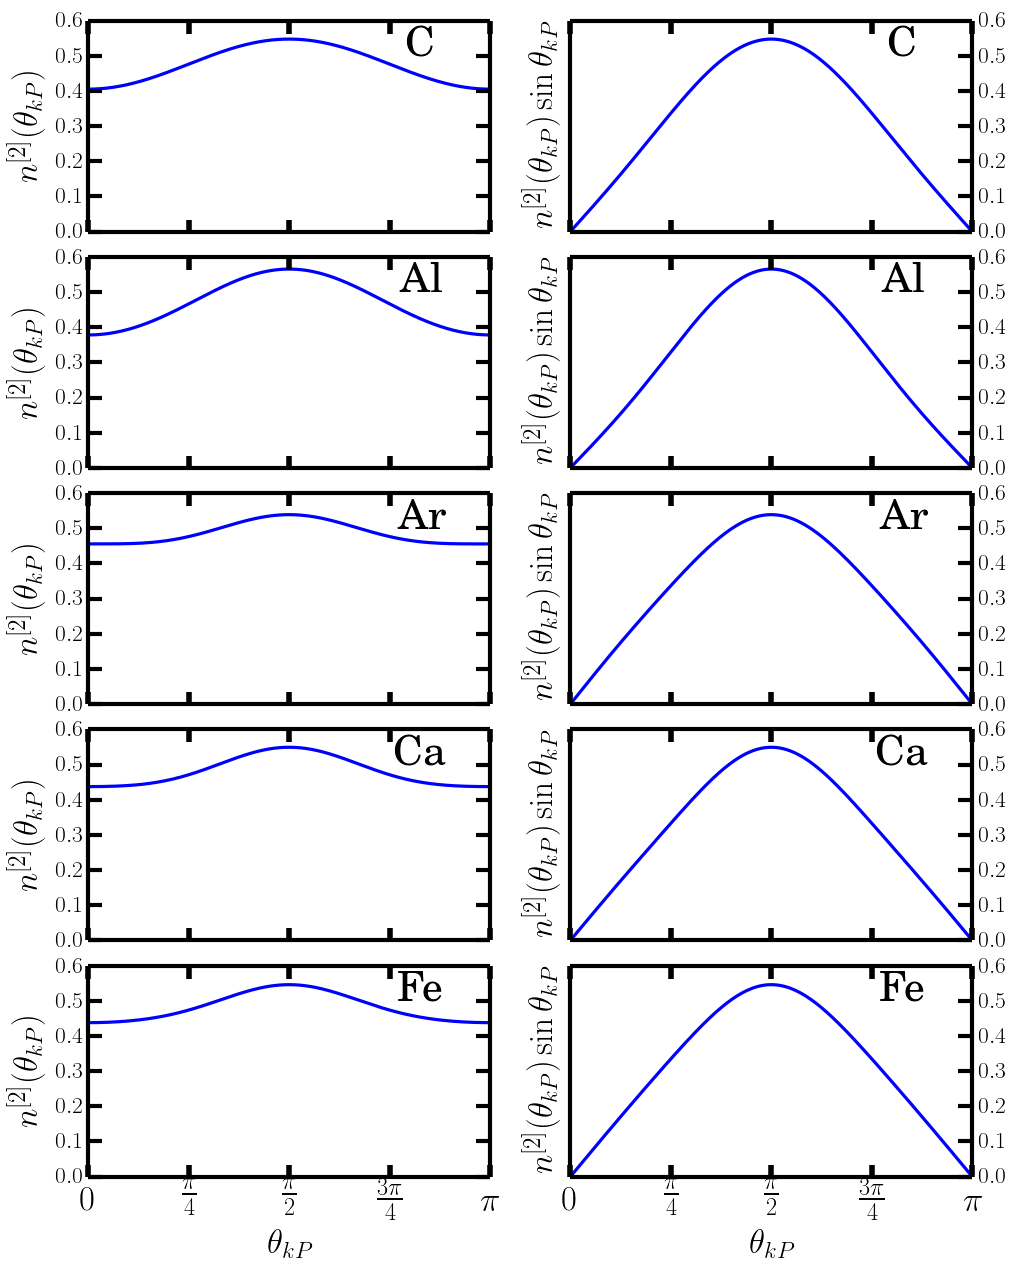
\includegraphics[scale=0.63]{./figuren/multi_angle.png}
\caption{Hoekdistributies $n^{[2]}(\theta_{kP})$ en $n^{[2]}(\theta_{kP})\sin{\theta_{kP}}$ van tweedeeltjes impuls waarbij $n^{[2]}(\theta_{kP})$ gegeven door uitdrukking \eqref{eq:angle_tb2}. De normalisatie is zodanig dat $\int d\theta_{kP}\ n^{[2]}(\theta_{kP})\sin{\theta_{kP}} = 1$.}
\label{fig:angle}
\end{figure}

\begin{figure}
\centering
\begin{subfigure}{0.49\textwidth}
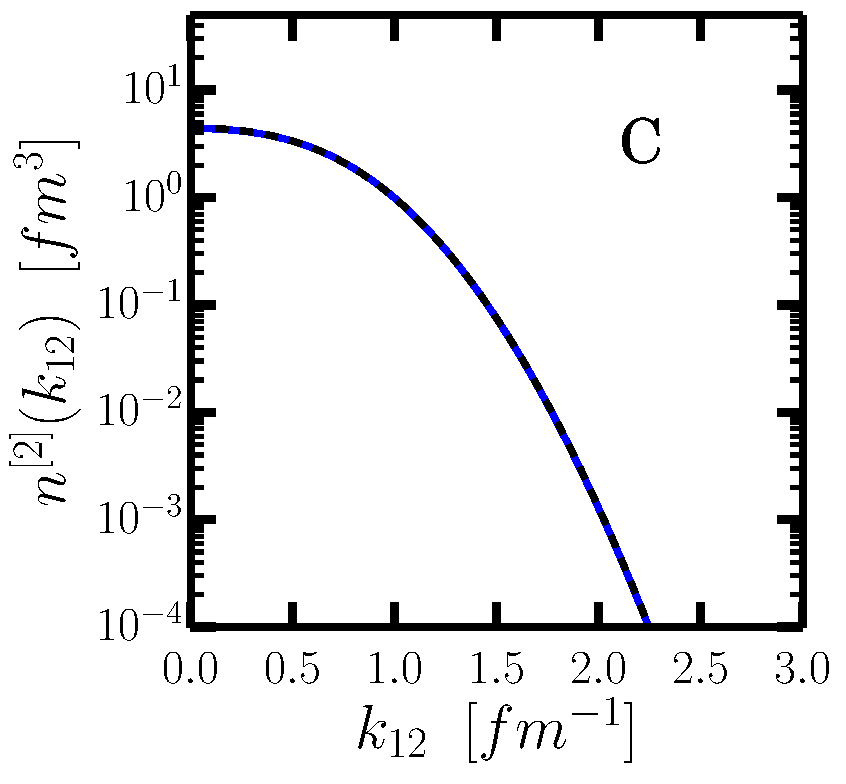
\includegraphics[width=\textwidth]{./figuren/C_tb_rel.pdf}
\end{subfigure}
\begin{subfigure}{0.49\textwidth}
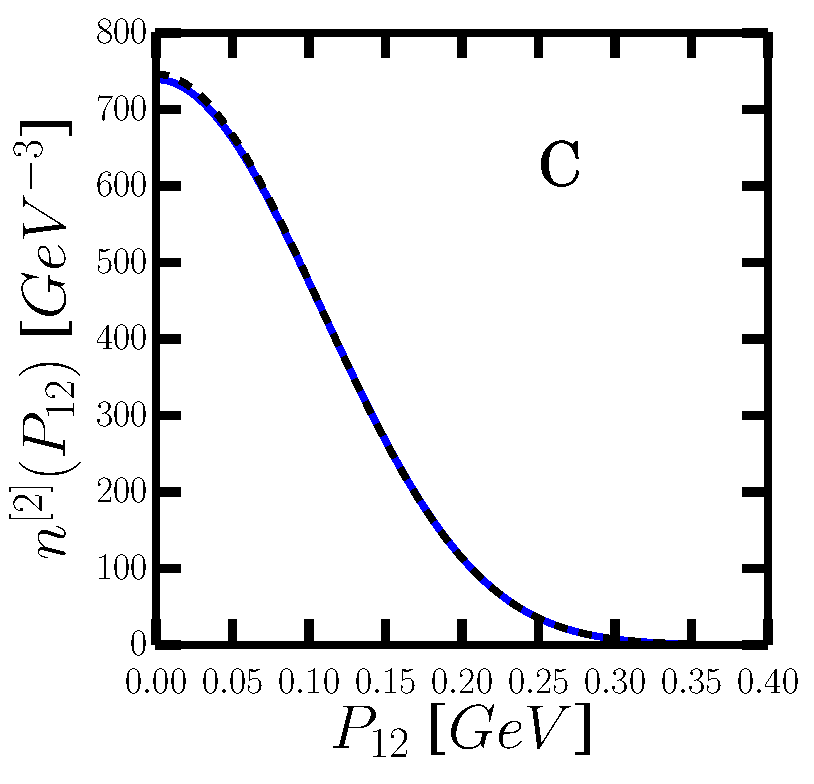
\includegraphics[width=\textwidth]{./figuren/C_tb_cm.pdf}
\end{subfigure}
\begin{subfigure}{0.49\textwidth}
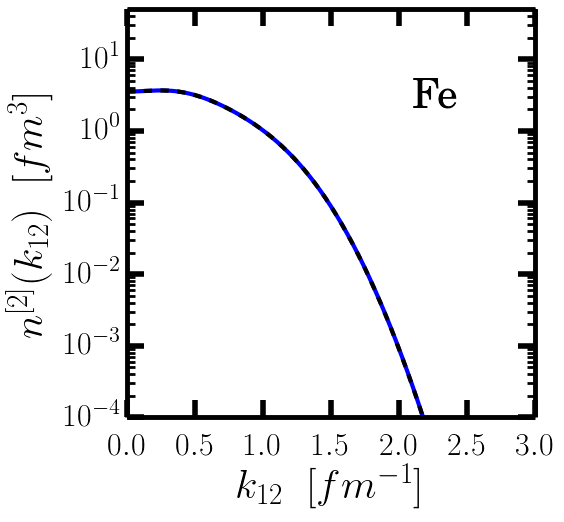
\includegraphics[width=\textwidth]{./figuren/Fe_tb_rel.png}
\end{subfigure}
\begin{subfigure}{0.49\textwidth}
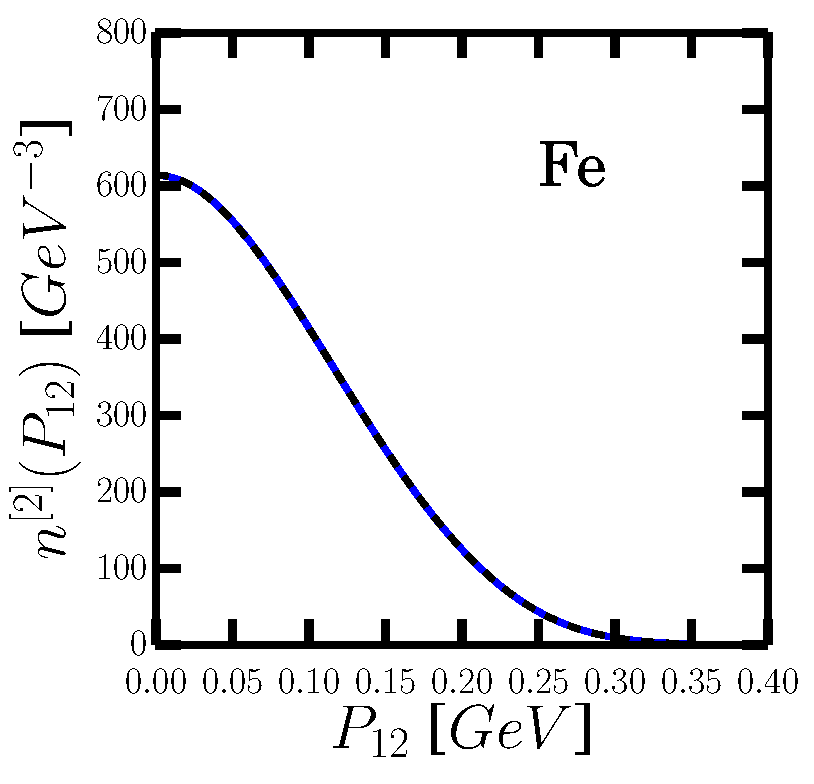
\includegraphics[width=\textwidth]{./figuren/Fe_tb_cm.pdf}
\end{subfigure}
\caption{Vergelijking van resultaten voor $n^{[2]}(k_{12})$ (links) en $n^{[2]}(P_{12})$ (rechts) met resultaten uit \cite{maarten}. De gestreepte curve is het resultaat bekomen door \cite{maarten} en de blauwe curve ons resultaat. }
\label{fig:vergelijking}
\end{figure}



\chapter{Wignerdistributie} \label{hfdstk:wigner}
\section{Algemene kenmerken}
Een klassiek deeltje wordt in de faseruimte ($(\vec{r},\vec{k})$-ruimte) voorgesteld door een punt, het heeft op elk tijdstip een welbepaalde impuls en positie. Een netto inwerkende kracht zorgt ervoor dat het deeltje een traject beschrijft in de faseruimte. Voor een ensemble van klassieke deeltjes kan de kans op het vinden van een deeltje in een bepaald punt van de faseruimte beschreven worden door een probabiliteitsdistributie $P(\vec{r},\vec{k})$. Een probabiliteit is steeds niet-negatief dus kan $P$ is een positief-definiete functie.  De gemiddelde waarde van een observabele $O(\vec{r},\vec{k})$ wordt berekend aan de hand van
\begin{equation} \label{eq:average_obs}
O_{av} = \int d\vec{r} \int d\vec{k}\ P(\vec{r},\vec{k})\ O(\vec{r},\vec{k})
\end{equation}
waarbij de integratie gaat over de volledige faseruimte.
In een kwantumsysteem worden de positie en impuls operatoren, respectievelijk $\hat{\vec{r}}$ en $\hat{\vec{k}}$,  die voldoen aan het onzekerheidsbeginsel van Heisenberg: 
\begin{equation} \label{eq:heisenberg}
\Delta x \Delta k \geq \frac{1}{2}
\end{equation}
waarbij  $\Delta O = \sqrt{\braket{\hat{O}^2}-\braket{\hat{O}}^2}$. $\braket{\hat{O}}$ is de verwachtingswaarde van operator $\hat{O}$. De oorsprong van deze ongelijkheid ligt in het niet commuteren van $\hat{\vec{r}}$ en $\hat{\vec{k}}$, namelijk
\begin{equation}
[\hat{\vec{r}}, \hat{\vec{k}} ] = i,
\end{equation}
met $i$ de imaginaire eenheid.
Daar een punt in de faseruimte een welbepaalde positie en impuls heeft, faalt de beschrijving van een kwantumsysteem met een klassieke probabiliteitsdistributie $P(\vec{r},\vec{k})$. Deze zou het onzekerheidsbeginsel \eqref{eq:heisenberg} schenden. In een klassiek systeem zijn observabelen getallen, geen operatoren, en commuteren bijgevolg altijd. Een voorstelling van een kwantumsysteem in de faseruimte wordt gegeven door een quasiprobabiliteitsdistributie. Een voorbeeld hiervan is de Wignerdistributie. Dit kwantummechanische analogon van de klassieke probabiliteitsdistributie verliest echter de fysische interpretatie als probabiliteit en wordt dus beschouwd als een zuiver mathematisch hulpmiddel voor de berekening van verwachtingswaarden. In tegenstelling tot een klassieke probabiliteitsdistributie kan een quasidistributie negatieve waarden aannemen die worden gelinkt aan kwantumeffecten. Men kan bewijzen dat deze gebieden met negatieve quasidistributie steeds klein zijn en verdwijnen in de klassieke limiet $\hbar \rightarrow 0$. De Wignerdistributie laat dus toe een vergelijking te maken met een analoog klassiek systeem en vertelt waar in de faseruimte kwantumeffecten een rol spelen.
Wignerdistributies hebben een relevantie bij verstrooiingsexperimenten aan gebonden nucleonen in de kern. Er zijn experimenten die impulsdistributies meten in regionen die kleiner zijn dan het volledige nucleaire volume. Bij verstrooiing aan een gebonden nucleon in een kern observeert men de \'{e}\'{e}ndeeltjes impulsdistributies van een nucleon in een beperkt volume \cite{Griffiths}.
De Wignerdistributie van een HO toestand gekarakteriseerd door een set kwantumgetallen $j = \{n,l,m\}$ defini\"{e}ren we als
\begin{equation} \label{eq:wigner_definitie}
W_{j}(\vec{r},\vec{k}) = \frac{1}{(2\pi)^3} \int d\vec{r}^{\ \prime} \ \phi_{j}^*\left(\vec{r}-\frac{\vec{r}^{\ \prime}}{2}\right) \phi_{j}\left(\vec{r}+\frac{\vec{r}^{\ \prime}}{2}\right)\  e^{-i\vec{k}\cdot \vec{r}^{\ \prime}} 
\end{equation} 
in overeenkomst met de definitie van E. Wigner die deze functie introduceerde \cite{wigner1932quantum}.
De bijhorende marginale distributies
\begin{equation}
\int d\vec{r}\ W_{j}(\vec{r},\vec{k}) =  \abs{\phi_{j}(\vec{k})}^2
\end{equation}
\begin{equation}
\int d\vec{k}\ W_{j}(\vec{r},\vec{k}) =  \abs{\phi_{j}(\vec{r})}^2,
\end{equation}
zijn respectievelijk de impuls- en dichtheidsdistributie van de $j$-toestand. Bijgevolg is normalisatie 
\begin{equation}
\int d\vec{r}\int d\vec{k}\ W_{j}(\vec{r},\vec{k}) = 1
\end{equation}
en $W_j$ is dimensieloos.
De Wignerdistributie is een voorbeeld van een Weyltransformatie van een operator $\hat{O}$:
\begin{equation}
\widetilde{O}(\vec{r},\vec{k}) = \int d\vec{r}^{\ \prime}\  \Braket{\vec{r} + \frac{\vec{r}^{\ \prime}}{2} | \hat{O}|  \vec{r} -\frac{\vec{r}^{\ \prime}}{2}} e^{-i \vec{k} \cdot \vec{r}^{\ \prime}}. 
\end{equation}
De Weyltransfromatie zet een operator, die normaliter inwerkt op een golffunctie, om naar een functie van $\vec{r}$ en $\vec{k}$.  Men kan bewijzen dat de integraal over de volledige faseruimte van het product van twee getransformeerde operatoren gelijk is aan het spoor van het product van deze operatoren,
\begin{equation} \label{eq:trace}
Tr[\hat{O}_1 \hat{O}_2] = \int d\vec{r} \int d\vec{k}\  \widetilde{O}_1(\vec{r},\vec{k}) \widetilde{O}_2(\vec{r},\vec{k}).
\end{equation}
Daar de dichtheidsoperator de gedaante
\begin{equation} \label{eq:dens_operator}
\hat{\rho} = \sum_j \ket{j} \bra{j}
\end{equation}
heeft, volgt dat
\begin{equation}
Tr[\hat{\rho}\hat{O}] =  \sum_j Tr[\ket{j} \bra{j} \hat{O}] = \sum_j Tr[\bra{j} \hat{O} \ket{j} ] = \braket{\hat{O}}.
\end{equation}
Hierbij werd gebruik gemaakt van de invariantie van een spoor onder cyclische permutatie en het feit dat het spoor van een getal niets anders is dan het getal zelf. Met dit in het achterhoofd en met behulp van relatie \eqref{eq:trace} kunnen we, eens de Wignerdistributie gekend is,  de verwachtingswaarde van een operator berekenen:
\begin{equation}
\braket{\hat{O}} = \int d\vec{r} \int d\vec{k}\  W(\vec{r},\vec{k}) \widetilde{O}(\vec{r},\vec{k})
\end{equation}
waarbij
\begin{align*}
 W(\vec{r},\vec{k}) \equiv \widetilde{\rho}(\vec{r}).
\end{align*}
De totale Wignerdistributie van het systeem is dus de Weylgetransformeerde van de dichtheidsoperator. Merk op dat uitdrukking dat gemiddelde waarden van observabelen in een klassiek systeem op dezelfde manier berekend worden (zie vergelijking \eqref{eq:average_obs}).
De relatie met de \'{e}\'{e}ndeeltjes impulsdistributie
\begin{equation} \label{eq:ob_function2}
n^{[1]}(\vec{k})=\frac{1}{(2\pi)^3}\int d\vec{r}_1 \int d\vec{r}_1^{\ \prime}\  e^{i\vec{k}\cdot (\vec{r}_1-\vec{r}^{\ \prime}_1)}\rho_1(\vec{r}_1,\vec{r}_1^{\ \prime})
\end{equation}
wordt duidelijk door de volgende transformatie van co\"{o}rdinaten:
\begin{align*}
\vec{r}^{\ \prime} & = \vec{r}^{\ \prime}_1-\vec{r}_1 \\
\vec{r} & = \frac{\vec{r}^{\ \prime}_1-\vec{r}_1}{2}
\end{align*}
De \'{e}\'{e}ndeeltjes impulsdistributie kan dan in direct verband gebracht worden met de Wignerdistributie:
\begin{align} \label{eq:voorwaarde}
n^{[1]}(\vec{k}) & =\frac{1}{(2\pi)^3}\int d\vec{r} \int d\vec{r}^{\ \prime}\  e^{-i\vec{k}\cdot\vec{r}^{\ \prime}}\rho_1(\vec{r}-\vec{r}^{\ \prime}/2,\vec{r}+\vec{r}^{\ \prime}/2) \nonumber \\
& = \int d\vec{r}\  W(\vec{r},\vec{k}).
\end{align}
Uit \eqref{eq:dens_operator} en de definitie van de Wignerdistributie van een toestand \eqref{eq:wigner_definitie} volgt dat de totale distributie van een kern niets anders is dan de som van de distributies van de individuele toestanden:
\begin{equation} \label{eq:wigner_magnitude}
 W(r,k) = \frac{2}{A}\sum_{\tau = -1/2}^{+1/2} (2l+1) \sum_{nl} \gamma_{nl} W_{nl}(r,k) 
\end{equation}
met 
\begin{equation} \label{eq:wigner_level}
W_{nl}(r,k) = \int d\Omega_r \int d\Omega_k\ \frac{1}{2l+1} \sum_{m= -l}^{l}W_{nlm}(\vec{r},\vec{k}).
\end{equation}
De sommatie gaat dan over ale bezette \'{e}\'{e}ndeeltjestoestanden $nl$ van de kern. Aangezien voor een bepaalde $l$ de verschillende $m  = -l, \ldots, l$ energetisch ontaard zijn in ons model nemen we een gemiddelde over deze toestanden zodat
\begin{equation}
K^{2}_{nl}(k) =   \int_0^\infty dr\ r^2\ W_{nl}(r,k)
\end{equation}
en
\begin{equation} \label{eq:voorwaarde_2}
n^{[1]}(k) =  \int_0^\infty dr\ r^2\  W(\vec{r},\vec{k}).
\end{equation}
\section{Resultaten}



Resultaten zijn te vinden in Figuren \ref{fig:wigner_plots} en \ref{fig:wigner_plots2}. Naast de Wignerdistributie $W(r,k)$ tonen we ook nog $W(r,k)r^2 k^2$. De kans (probabiliteit) om een deeltje te vinden op een afstand $r$ van het centrum van de kern wordt gegeven door 
\begin{equation}
\rho (r) = r^2 \int dk\ k^2 W(r,k).
\end{equation}
Bijgevolg wordt $W(r,k)r^2 k^2$ gedefinieerd als quasiprobabiliteit.

Een eerste opvallende eigenschap is dat alle berekende distributies oscillatorisch gedrag vertonen. Daar de totale Wignerdistributie in een ODM de som is van de Wignerdistributies van de bezette \'{e}\'{e}ndeeltjestoestanden tonen we deze individuele bijdragen in Figuur \ref{fig:wigner_iron} voor een ijzerkern. Uit deze distributies valt dan op dat het aantal nodes toeneemt met de energie van de toestand, bepaald door $N=2n+l$. Het is zelfs zo dat het aantal nodes gelijk is aan $N$, een eigenschap die volgt uit de golffuncties van de respectievelijke toestanden, die dezelfde eigenschap hebben. We merken echter op dat voor $n=1$ twee nodes samenkomen en een negatief gebied vormen.
De Wignerdistributies, op deze van grondtoestand na, hebben negatieve waarden. Kwantumeffecten spelen dus een rol n een kern.
Tenslotte merken we op dat het maximum van $W(r,k)r^2 k^2$ opschuift naar grotere $r$ naarmate we naar zwaardere kernen kijken. In $k$ is er geen duidelijke verschuiving. Dit volgt uit de bijdragen van de individuele \'{e}\'{e}ndeeltjestoestanden die dezelfde eigenschap vertonen.
Ter controle tonen we nog aan dat de berekende Wignerdistributies de correcte marginale distributies hebben (Figuur \ref{fig:test_ob}). We eisen namelijk dat de integratie van de  Wignerdistributie van een kern over alle $r$-afhankelijkheid gelijk is aan de \'{e}\'{e}ndeeltjes impulsdistributie van deze kern. Deze voorwaarde is geformuleerd in uitdrukking \eqref{eq:voorwaarde_2}.
\begin{figure}
\centering
 \begin{subfigure}[b]{0.49\textwidth} 
 	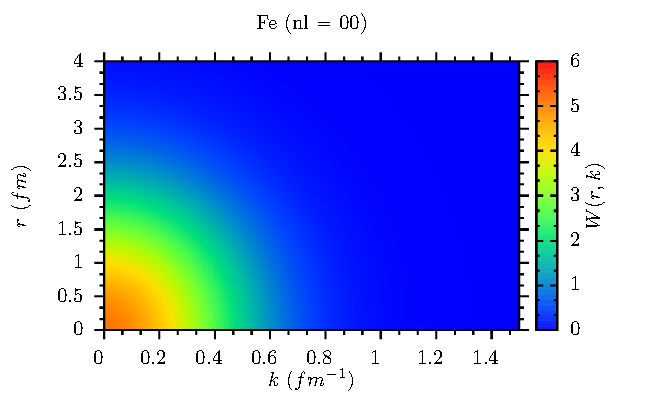
\includegraphics[width=\textwidth]{./figuren/Fe_wigner_00.pdf}  
 \end{subfigure}
 \begin{subfigure}[b]{0.49\textwidth} 
 	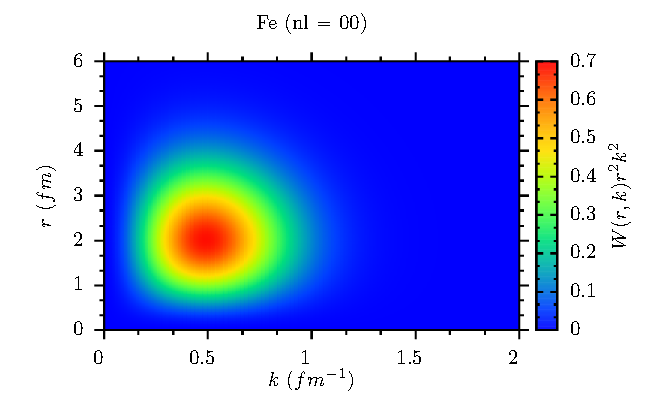
\includegraphics[width=\textwidth]{./figuren/Fe_wigner_00prob.pdf}  
 \end{subfigure}  
 \begin{subfigure}[b]{0.49\textwidth} 
 	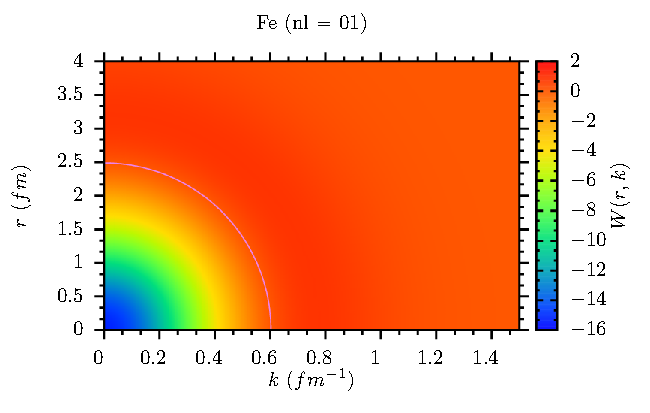
\includegraphics[width=\textwidth]{./figuren/Fe_wigner_01.pdf}  
 \end{subfigure} 
 \begin{subfigure}[b]{0.49\textwidth} 
 	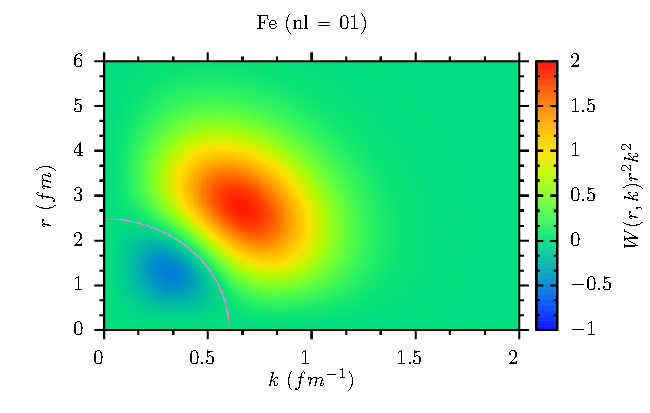
\includegraphics[width=\textwidth]{./figuren/Fe_wigner_01prob.pdf}  
 \end{subfigure} 
 \begin{subfigure}[b]{0.49\textwidth} 
 	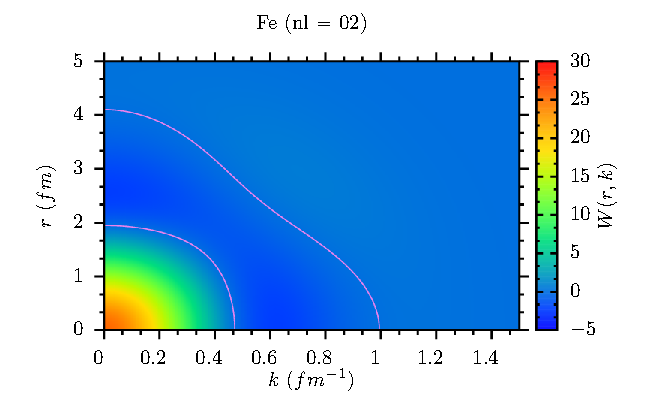
\includegraphics[width=\textwidth]{./figuren/Fe_wigner_02.pdf}  
 \end{subfigure}
 \begin{subfigure}[b]{0.49\textwidth} 
 	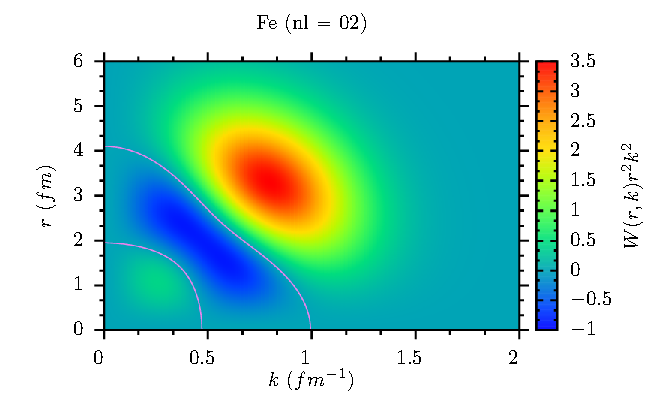
\includegraphics[width=\textwidth]{./figuren/Fe_wigner_02prob.pdf}  
 \end{subfigure} 
 \begin{subfigure}[b]{0.49\textwidth} 
 	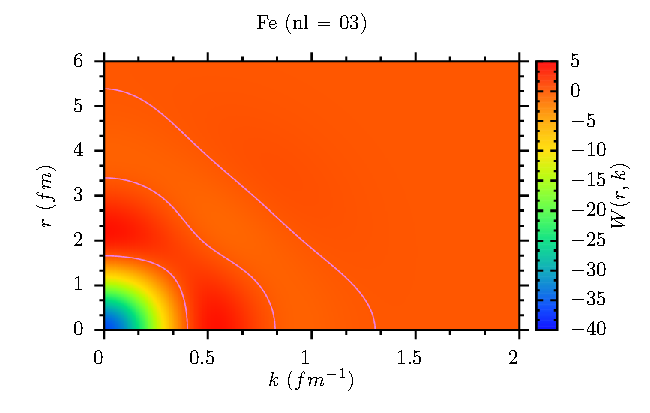
\includegraphics[width=\textwidth]{./figuren/Fe_wigner_03.pdf}  
 \end{subfigure} 
 \begin{subfigure}[b]{0.49\textwidth} 
 	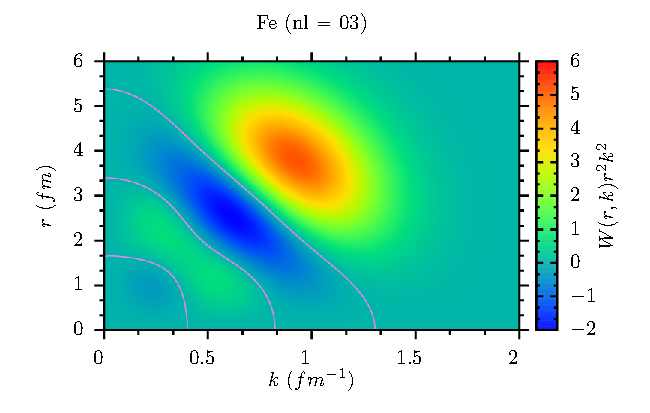
\includegraphics[width=\textwidth]{./figuren/Fe_wigner_03prob.pdf}  
 \end{subfigure} 
 \caption{Links: Wignerdistributies $W_{nl}(r,k)$, gegeven door uitdrukking \eqref{eq:wigner_level}, voor verschillende \'{e}\'{e}ndeeltjestoestanden in een ijzerkern (Fe). Let steeds op de schalen van $r$ en $k$, deze kunnen vari\"{e}ren van figuur tot figuur. Rechts: $W_{nl}(r,k)r^2 k^2$ voor elk van deze toestanden. De lichpaarse lijn stelt de nodes voor van de beschouwde functie om de negatieve gebieden beter in kaart te brengen.}  \label{fig:wigner_iron}
\end{figure}

\begin{figure} 
\centering
 \begin{subfigure}[b]{0.49\textwidth} 
 	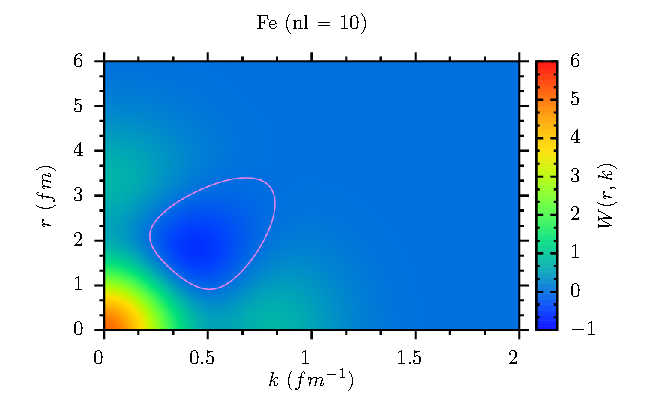
\includegraphics[width=\textwidth]{./figuren/Fe_wigner_10.pdf}  
 \end{subfigure}
 \begin{subfigure}[b]{0.49\textwidth} 
 	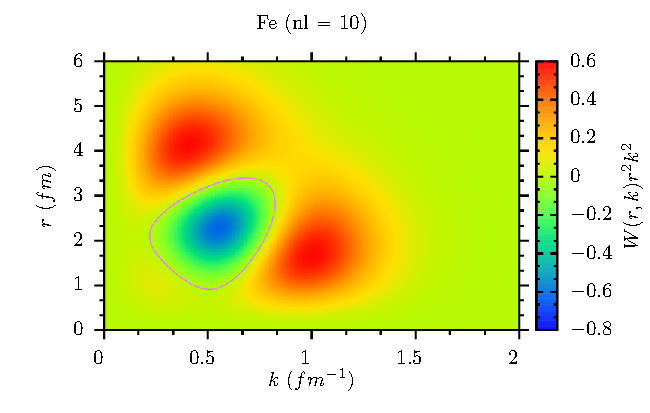
\includegraphics[width=\textwidth]{./figuren/Fe_wigner_10prob.pdf}  
 \end{subfigure} 
 \begin{subfigure}[b]{0.49\textwidth} 
 	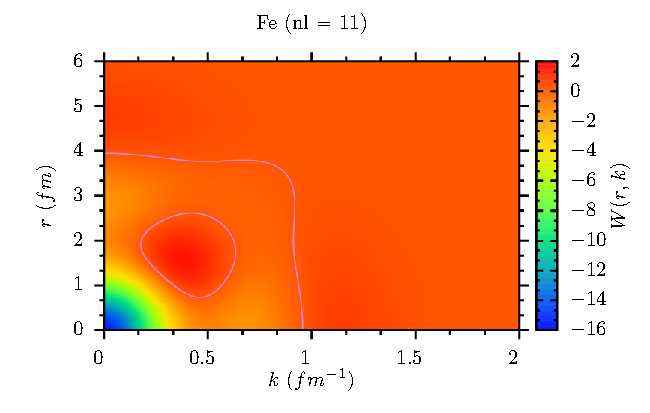
\includegraphics[width=\textwidth]{./figuren/Fe_wigner_11.pdf}  
 \end{subfigure} 
 \begin{subfigure}[b]{0.49\textwidth} 
 	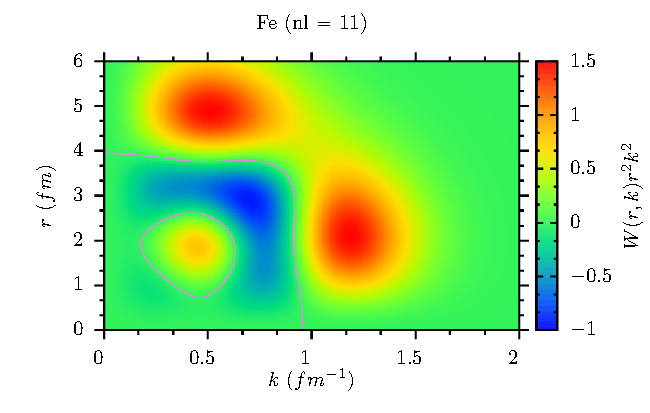
\includegraphics[width=\textwidth]{./figuren/Fe_wigner_11prob.pdf}  
 \end{subfigure} 
 \caption{Links: Wignerdistributies $W_{nl}(r,k)$, gegeven door uitdrukking \eqref{eq:wigner_level}, voor verschillende \'{e}\'{e}ndeeltjestoestanden in een ijzerkern (Fe). Let steeds op de schalen van $r$ en $k$, deze kunnen vari\"{e}ren van figuur tot figuur. Rechts: $W_{nl}(r,k)r^2 k^2$ voor elk van deze toestanden. De lichpaarse lijn stelt de nodes voor van de beschouwde functie om de negatieve gebieden beter in kaart te brengen.}  \label{fig:wigner_iron2}
\end{figure}


\begin{figure} 
\centering
 \begin{subfigure}[b]{0.49\textwidth} 
 	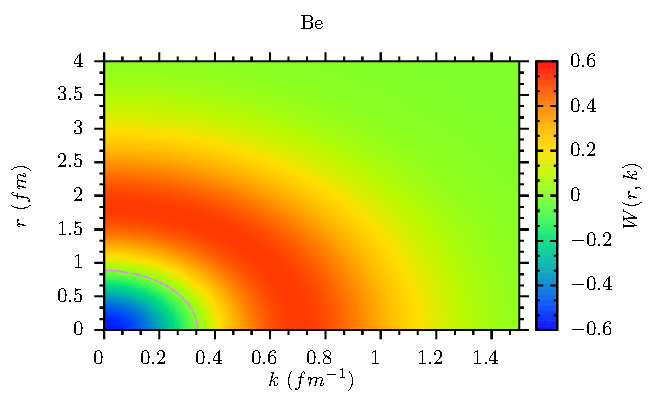
\includegraphics[width=\textwidth]{./figuren/Be.pdf}  
 \end{subfigure} 
 \begin{subfigure}[b]{0.49\textwidth} 
 	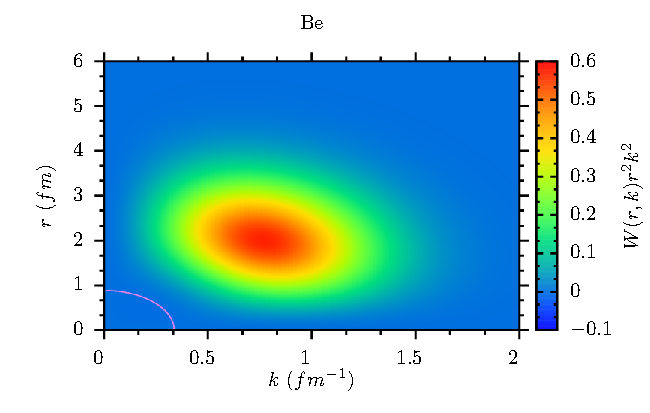
\includegraphics[width=\textwidth]{./figuren/Beprob.pdf}  
 \end{subfigure}  
 \begin{subfigure}[b]{0.49\textwidth} 
 	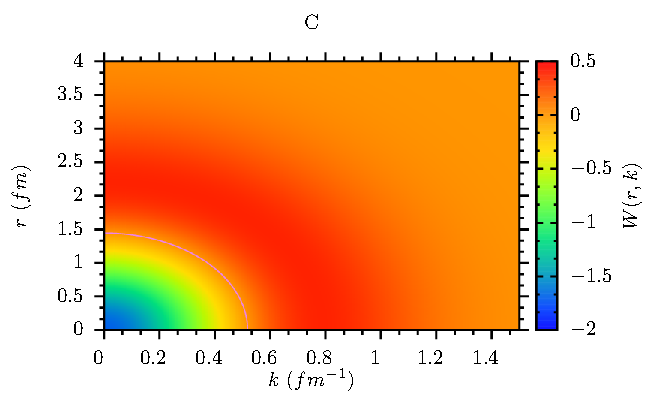
\includegraphics[width=\textwidth]{./figuren/C.pdf}  
 \end{subfigure}
 \begin{subfigure}[b]{0.49\textwidth} 
 	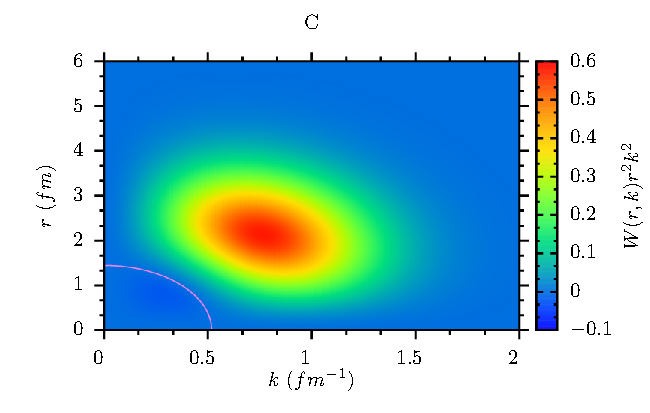
\includegraphics[width=\textwidth]{./figuren/Cprob.pdf}  
 \end{subfigure} 
 \begin{subfigure}[b]{0.49\textwidth} 
 	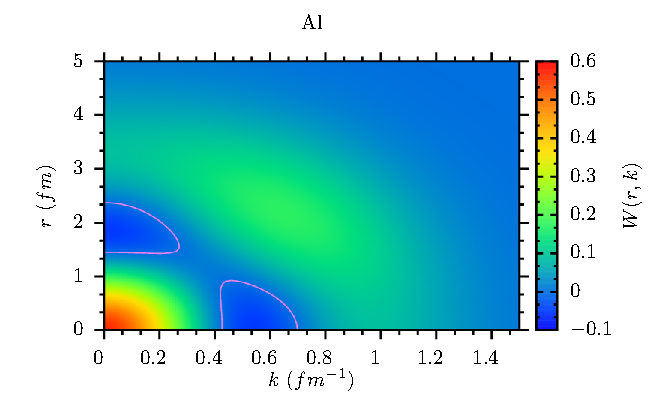
\includegraphics[width=\textwidth]{./figuren/Al.pdf}  
 \end{subfigure} 
 \begin{subfigure}[b]{0.49\textwidth} 
 	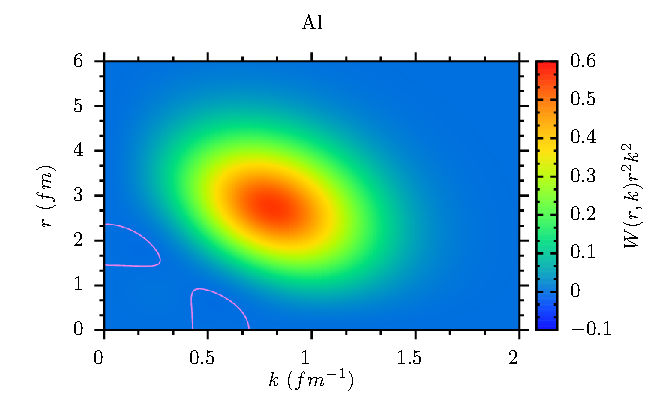
\includegraphics[width=\textwidth]{./figuren/Alprob.pdf}  
 \end{subfigure} 
 \begin{subfigure}[b]{0.49\textwidth} 
 	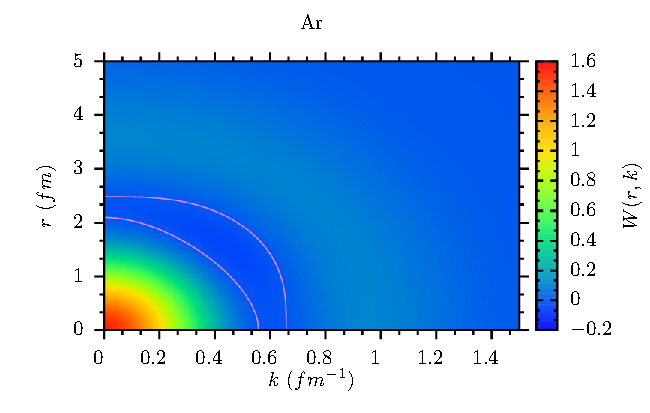
\includegraphics[width=\textwidth]{./figuren/Ar.pdf}  
 \end{subfigure}
 \begin{subfigure}[b]{0.49\textwidth} 
 	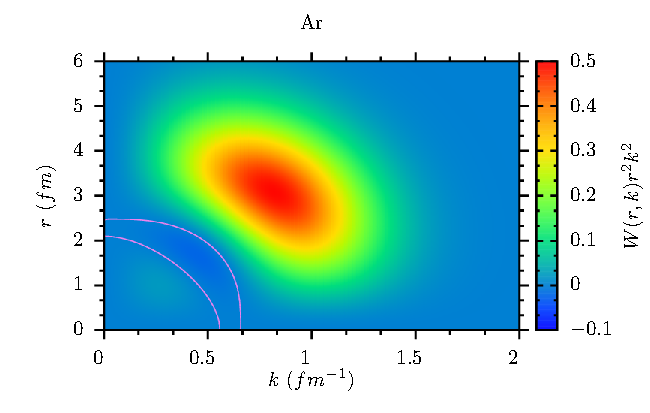
\includegraphics[width=\textwidth]{./figuren/Arprob.pdf}  
 \end{subfigure}
 \caption{Links: Wignerdistributies $W_{nl}(r,k)$ gegeven door uitdrukking \eqref{eq:wigner_magnitude}, voor $  \nuclide[9][4]{Be} \nuclide[12][6]{C}, \nuclide[27][13]{Al}$ en $\nuclide[40][18]{Ar}$. Let steeds op de schalen van $r$ en $k$. Rechts: de bijhorende $W_{nl}(r,k)r^2 k^2$. De lichpaarse lijn stelt de nodes voor van de beschouwde functie om de negatieve gebieden beter in kaart te brengen.}  \label{fig:wigner_plots}
\end{figure}


\begin{figure}
\centering
 \begin{subfigure}[b]{0.49\textwidth} 
 	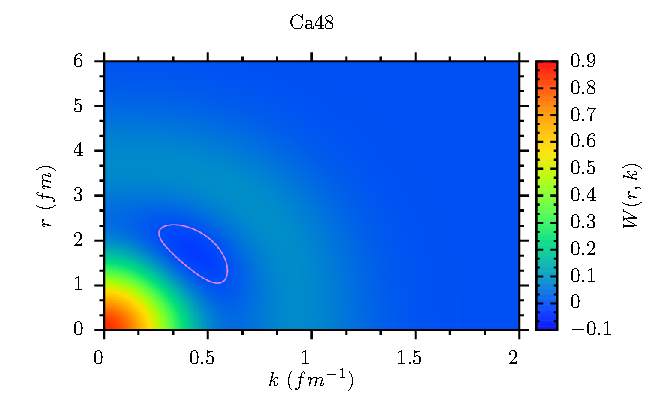
\includegraphics[width=\textwidth]{./figuren/Ca48.pdf}  
 \end{subfigure} 
 \begin{subfigure}[b]{0.49\textwidth} 
 	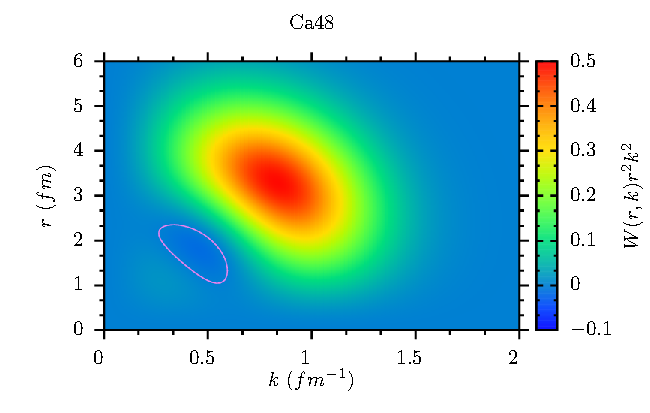
\includegraphics[width=\textwidth]{./figuren/Ca48prob.pdf}  
 \end{subfigure} 
 \begin{subfigure}[b]{0.49\textwidth} 
 	\includegraphics[width=\textwidth]{./figuren/Fe.pdf}  
 \end{subfigure} 
 \begin{subfigure}[b]{0.49\textwidth} 
 	\includegraphics[width=\textwidth]{./figuren/Feprob.pdf}  
 \end{subfigure} 
 \caption{Links: Wignerdistributies $W_{nl}(r,k)$, gegeven door uitdrukking \eqref{eq:wigner_magnitude}, voor $\nuclide[48][20]{Ca}$ en $\nuclide[56][26]{Fe}$. Let steeds op de schalen van $r$ en $k$. Rechts: de bijhorende $W_{nl}(r,k)r^2 k^2$. De lichpaarse lijn stelt de nodes voor van de beschouwde functie om de negatieve gebieden beter in kaart te brengen.}   \label{fig:wigner_plots2}
\end{figure}

\begin{figure}
\centering
 \begin{subfigure}[b]{0.49\textwidth} 
 	\includegraphics[width=\textwidth]{./figuren/C_ob_test.pdf}  
 \end{subfigure} 
 \begin{subfigure}[b]{0.49\textwidth} 
 	\includegraphics[width=\textwidth]{./figuren/Fe_ob_test.pdf}  
 \end{subfigure} 
 \caption{De volle blauwe curve is de \'{e}\'{e}ndeeltjes impulsdistributie berekend in Hoofdstuk \ref{eendeeltjes}(vergelijking \eqref{eq:ob_magnitude}). De gestreepte curve stelt $\int dr\ W(r,k)r^2$ voor met $W(r,k)$ gegeven door uitdrukking \eqref{eq:wigner_magnitude}. We zien dat voorwaarde \eqref{eq:voorwaarde_2} is voldaan. }
   \label{fig:test_ob}
\end{figure}

\chapter{Conclusie en vooruitzichten}
In dit hoofdstuk worden de besluiten uit bovenstaande onderzoeken gegeven en afsluitend bespreken we nog enkele mogelijkheden voor verder onderzoek.

\section{Conclusie}
In een ODM is de \'{e}\'{e}ndeeltjes impulsdistributie een som van individuele bijdragen van de bezette orbitalen in een kern. Deze distributies vertonen niet-Gaussische kenmerken zoals een zekere scheefheid en kurtosis. Echter, deze afwijkingen zijn klein genoeg om te zeggen dat de \'{e}\'{e}ndeeltjes impuls in een ODM goed beschreven wordt door een normale verdeling. Een normale verdeling heeft steeds een eindige probabiliteit heeft voor een negatieve grootte van de impuls. Echter de grootte van de impuls moet steeds positief zijn. We kunnen de distributies beter beschrijven met een functie $P(k) \propto k^\alpha P_{normal}(k)$ die steeds nul is bij $k=0$. De parameter $\alpha$ wordt gefit aan de theoretische curve. Voor massagetal $A \rightarrow0$ komen we steeds dichter bij $\alpha = 2$, een Maxwell-Boltzmannverdeling. Voor zwaardere kernen wordt $\alpha$ heel klein. De gemiddelde kinetische energie van een neutron en een proton in een kern, berekend aan de hand van de respectievelijke \'{e}\'{e}ndeeltjes impulsdistributies, ligt onder de waarde gegeven door een Fermi-model ($\braket{T}= 21\ MeV$). Ook modellen met correlaties tussen de nucleonen geven een hogere waarde omdat correlaties een brede staart bij hoge impuls introduceren ($k \gtrsim 2 fm^{-1}$) en de gemiddelde kinetische energie afhankelijk is van het vierde moment van de impulsdistributie.
 
 
Als we naar de impuls van twee nucleonen kijken in een ODM kunnen we onderscheid maken tussen relatieve impuls die de twee nucleonen hebben ten opzichte van elkaar en de impuls van hun massacentrum. Zowel de verdeling van de relatieve impuls als de impuls van hun massacentrum is bij benadering Gaussisch. Uit vergelijking met resultaten berekend in een model met correlaties blijkt dat vooral $l=0$ wordt be\"{i}nvloed door correlaties, die in de totale distributies voor een brede staart zorgen bij hoge impulsen. GV-berekeningen zijn hier relevant voor $k_{12}, P_{12} \lesssim 1.5 fm^{-1}$.
Uit de verdeling van de hoek tussen de relatieve impuls en de impuls van het massacentrum van twee nucleonen leren we dat twee nucleonen voornamelijk in een toestand voorkomen waarbij deze hoek $\frac{\pi}{2}$ is, een loodrechte configuratie. Daaruit volgt dat in een systeem van twee nucleonen de individuele impulsen bij voorkeur even groot zijn.

Tenslotte werden nog de Wignerdistributies van kernen uitgerekend welke een beeld geven van de faseruimte van nucleonen in een kern.
Deze distributies vertonen oscillatorisch gedrag en het maximum van de quasiprobabiliteit schuift steeds op naar grotere $r$ voor grotere kernen.


\section{Vooruitzichten}

Eerst en vooral zou men andere golffuncties kunnen gebruiken, bijvoorbeeld eigenfuncties van de Schr\"{o}dingervergelijking met een WS potentiaal. Deze kunnen dan ontwikkeld worden in een basis van HO eigenfuncties zodat we nog steeds de handige eigenschappen van deze laatste kunnen gebruiken. Echter kwalitatief verwacht men een analoge uitkomst.
Een ODM is een relatief goede benadering voor een kern maar het heeft beperkingen. Correlaties blijken essenti\"{e}el om de experimenteel gemeten impulsdistributies te verklaren voor grote impuls. Er is echter reeds veel onderzoek gebeurd rond de invloed van deze correlaties, bijvoorbeeld in \cite{maarten,ryckebusch2015stylized,wiringa2014nucleon}.
Interessant zijn de tweedeeltjes Wignerdistributies die een beeld geven van de faseruimte van de relatieve beweging van twee nucleonen in een kern alsook de faseruimte van hun massacentrum.
Tenslotte lijkt het ook interessant om een transformatie naar commuterende variabelen toe te passen op de Wignerdistributie, een pseudo-positie en een pseudo-impuls die bijvoorbeeld normaal verdeeld zijn, respectievelijk, rond de echte positie en impuls. Zo kan men de Wignerdistributie transformeren naar een positief definiete functie die bijgevolg een probabiliteit voorstelt \cite{PhysRev.120.254}. 


\newpage
\appendix
\numberwithin{equation}{section}

\chapter{ Tweede kwantisatie} 
Kwantummechanica wordt meestal ge\"{i}ntroduceerd in een vorm die eerste kwantisatie heet. In de dit formalisme zijn golffuncties functie van de co\"{o}rdinaten van de bestudeerde objecten en elk van deze objecten krijgt dan een label. In tweede kwantisatie  is de formulering echter zodanig  dat er geen labels zijn. Dus we spreken niet meer over deeltje 1, deeltje 2, ... . Dus in zekere zin sluit het tweede kwantisatie formalisme deze niet-fysische informatie uit. Het formalisme is heel handig om veeldeeltjessystemen te beschrijven. In de volgende sectie geven we de gebruikte conventies mee. We baseren ons hierbij op het hoofdstuk $Second\ quantization$ uit \cite{dimitri}.
\section{Conventies} \label{sec:tweede_kwant}
We schrijven de toestandsvector van een kern in tweede kwantisatie als 
\begin{equation}
\ket{n_1, n_2, n_3 , \ldots}
\end{equation}
waarbij $n_\alpha$ is het aantal deeltjes in het \'{e}\'{e}ndeeltjes orbitaal $u_\alpha$.
Creatie- en annihilatie-operatoren worden respectievelijk gedefinierd als  $c^\dagger_\alpha$ en  $c_\alpha$. De creatie-operator $c^\dagger_\alpha$ voegt \'{e}\'{e}n deeltje toe aan een \'{e}\'{e}ndeeltjes orbitaal $u_\alpha$  en $c_\alpha$ verwijdert \'{e}\'{e}n deeltje uit dit orbitaal:
\begin{align}
c^\dagger_\alpha\ket{n_1, n_2, \ldots, n_i, \ldots} & = \left(\mathds{1} \otimes \mathds{1} \otimes \cdots \otimes c^\dagger_\alpha \otimes  \cdots \otimes \mathds{1} \right) \ket{n_1} \otimes \ket{n_2} \otimes \cdots \otimes \ket{n_\alpha} \otimes \cdots \\
& = (-1)^{s_\alpha}\ket{n_1} \otimes \ket{n_2} \otimes \cdots \otimes c^\dagger_\alpha \ket{n_\alpha} \otimes \cdots \\
& = \delta_{0n_\alpha}(-1)^{s_\alpha}\ket{n_1, \ldots, n_{\alpha-1},  n_\alpha+1,  n_{\alpha+1}, \ldots }.
\end{align}
waarbij
\begin{equation}
s_\alpha= n_1 + n_2 + \ldots + n_{\alpha-1}
\end{equation}
en de Kronecker delta ervoor zorgt dat het Pauli-principe voldaan is. De factor $(-1)^{s_\alpha}$ volgt uit de anticommutatierelaties voor fermionen:
\begin{align}
& \{c_\alpha, c^\dagger_\beta \} = \delta_{\alpha \beta} \\
& \{c_\alpha, c_\beta \} =\{c^\dagger_\alpha, c^\dagger_\beta \}  = 0.
\end{align}
Relaties voor de annihilatie-operatoren volgen uit dezelfde principes: 
\begin{equation}
c_\alpha \ket{n_1, n_2, \ldots, n_\alpha, \ldots} = \delta_{1n_\alpha}(-1)^{s_\alpha}\ket{n_1, \ldots, n_{\alpha-1},  n_\alpha-1,  n_{\alpha+1}, \ldots }.
\end{equation}
De teloper teloperator  wordt gedefinieerd als
\begin{equation}
\hat{N} = \sum_\alpha c^\dagger_\alpha c_\alpha
\end{equation}
en heeft eigenwaarden N $\in \mathds{N}$  en eigenfuncties zijn golffuncties met een vast aantal deeltjes. Een genormaliseerde veeldeeltjestoestand kan gecre\"{e}rd worden door creatie-operatoren op de grondtoestand te laten inwerken:
\begin{equation}
\ket{n_1, n_2, n_3 , \ldots} = (c^\dagger_1)^{n_1} (c^\dagger_2)^{n_2} \cdots \ket{0}.
\end{equation}
Voor fermionen zijn deze toestanden op \'{e}\'{e}n genormeerd en de $n_i$'s zijn 0 of 1. We kiezen een speciefieke volgorde van de \'{e}\'{e}ndeeltjestoestanden ${u_\alpha}$ en houden deze vast.

Een deeltje cre\"{e}ren op een plaats $\vec{r}$ wordt gebeurt door de operator
\begin{align}
\psi^\dagger(\vec{r}) = \sum_\alpha c^\dagger_\alpha  u^*_\alpha(\vec{r})
\end{align}
waarbij
\begin{equation}
c^\dagger_\alpha = \int d\vec{r}\ \psi^\dagger(\vec{r}) u^*_\alpha(\vec{r}).
\end{equation}
Men kan bovenstaande definitie controleren door een deeltje te cre\"{e}ren in toestand $\alpha$:
\begin{align}
\ket{\alpha} & = \int d\vec{r}\ u_\alpha(\vec{r}) \ket{\vec{r}} \\
 & = \int d\vec{r}\ u_\alpha(\vec{r}) \psi^\dagger(\vec{r}) \ket{0} \\
 & = \int d\vec{r}\ u_\alpha(\vec{r}) \sum_\beta c^\dagger_\beta  u^*_\beta(\vec{r}) \ket{0} \\
 & = c^\dagger_\alpha \ket{0}.
\end{align}
Bij de laatste stap maakten we gebruik van de orthonormaliteit van de \'{e}\'{e}ndeeltjesorbitalen:
\begin{equation}
\int d\vec{r}\ u_\alpha(\vec{r}) u^*_\beta(\vec{r}) = \delta_{\alpha \beta}.
\end{equation}
Men heeft ook nog de volgende  handige relaties:
\begin{align}
& u_\alpha(\vec{r})  = \braket{\vec{r}|\vec{\alpha}}  \\
& \braket{\vec{r}|\vec{r}^{\ \prime}} = \delta(\vec{r}-\vec{r}^{\ \prime}) \\
& \braket{\vec{r}|\vec{k}} = \frac{1}{(2\pi)^{3/2}} e^{i\vec{k}\cdot \vec{r}} \\
& \braket{\vec{k}|\vec{r}} = \frac{1}{(2\pi)^{3/2}} e^{-i\vec{k}\cdot \vec{r}}.
\end{align}

Nu wordt een genormaliseerde A-deeltjes Focktoestand in eerste kwantisatie: 
\begin{equation}
\ket{\vec{r}_1, \vec{r}_2, \ldots, \vec{r}_A } = \frac{1}{\sqrt{A!}} \psi^\dagger(\vec{r}_1) \psi^\dagger(\vec{r}_2) \cdots \psi^\dagger(\vec{r}_A) \ket{0}.
\end{equation}
En de golffunctie in de configuratieruimte:
\begin{equation}
\braket{\vec{r}_1, \vec{r}_2, \ldots, \vec{r}_A | n_1, n_2, n_3 , \ldots} = \Psi_A(\vec{r}_1, \vec{r}_2, \ldots, \vec{r}_A ).
\end{equation}

\section{E\'{e}ndeeltjes impulsoperator} \label{operator}

Hier geven we een bewijs van de uitdrukking  van de \'{e}\'{e}ndeeltjes impulsoperator in tweede kwantisatie die de eenvoudige interpretatie van een teloperator in de impulsruimte. We beginnen bij de definitie:
\begin{align}
n^{[1]}(\vec{k}) & =\frac{1}{(2\pi)^3}\int d\vec{r}_1 \int d\vec{r}_1^{\ \prime}\  e^{i\vec{k}\cdot (\vec{r}_1-\vec{r}^{\ \prime}_1)}\rho_1(\vec{r}_1,\vec{r}_1^{\ \prime})  \nonumber \\
& =\int d\vec{r}_1 \int d\vec{r}_1^{\ \prime}  \int d\{\vec{r}_{2-A}\} \braket{\vec{r}_1| \vec{k}} \braket{\vec{k}| \vec{r}_1^{\ \prime}} \braket{\Psi_A | \vec{r}_1, \{ \vec{r}_{2-A}\} } \braket{\vec{r}_1^{\ \prime}, \{ \vec{r}_{2-A}\}|\Psi_A  }   \nonumber \\
& = \frac{1}{A!} \int d\vec{r}_1 \int d\vec{r}_1^{\ \prime}  \int d\{\vec{r}_{2-A}\} \braket{\vec{r}_1| \vec{k}} \braket{\vec{k}| \vec{r}_1^{\ \prime}} \nonumber \\
&\phantom{{aaaa}=3} \times \bra{\Psi_A} \psi^\dagger(\vec{r}_1) \psi^\dagger(\vec{r}_2) \cdots \psi^\dagger(\vec{r}_A) \ket{0} \bra{0} \psi(\vec{r}_A) \cdots \psi(\vec{r}_2) \psi(\vec{r}_1^{\ \prime}) \ket{\Psi_A}.
\end{align}
De projectie op de vacu\"{u}mtoestand $\ket{0} \bra{0}$ kan vervangen worden door de eenheidsoperator omdat $\psi(\vec{r}) \; (\psi^\dagger(\vec{r}))$ reeds alle deeltjes in de ket (bra) vector heeft geannihileerd:
\begin{align}
n^{[1]}(\vec{k}) & = \frac{1}{A!} \int d\vec{r}_1^{\ \prime}  \int d{\vec{r}_{2-A}} \braket{\vec{r}_1| \vec{k}} \braket{\vec{k}| \vec{r}_1^{\ \prime}} \nonumber \\
&\phantom{{aaaa}=3} \times \bra{\Psi_A} \psi^\dagger(\vec{r}_1) \psi^\dagger(\vec{r}_2) \cdots \psi^\dagger(\vec{r}_A) \psi(\vec{r}_A) \cdots \psi(\vec{r}_2) \psi(\vec{r}_1^{\ \prime}) \ket{\Psi_A}.
\end{align}

Integratie over de coördinaten $\vec{r}_2$ tot $\vec{r}_A$ is triviaal aangezien $\int d\vec{r} \psi^\dagger(\vec{r}) \psi(\vec{r})$ de teloperator is in de configuratieruimte. Integratie over  $\vec{r}_A$ levert dus een factor  \'{e}\'{e}n omdat het inwerkt op een toestandsvector $\psi(\vec{r}_{A-1}) \cdots \psi(\vec{r}_2) \psi(\vec{r}_1) \ket{\Psi_A}$, waar alle deeltjes, op  \'{e}\'{e}n na, geannihileerd zijn. Om dezelfde redenen geeft de integratie over  $\vec{r}_{A-1}$ een factor 2. Als men dus integreert over alle co\"{o}rdinaten $\vec{r}_2$ tot $\vec{r}_A$, krijgt men een factor $(A-1)!$.  De  \'{e}\'{e}ndeeltjes impulsdistributie kan nu geschreven worden als
\begin{align}
n^{[1]}(\vec{k}) & = \frac{1}{A}  \int d\vec{r}_1\int d\vec{r}_1^{\ \prime}  \braket{\vec{r}_1| \vec{k}} \braket{\vec{k}| \vec{r}_1^{\ \prime}} \bra{\Psi_A} \psi^\dagger(\vec{r}_1) \psi(\vec{r}_1^{\ \prime}) \ket{\Psi_A}  \nonumber \\
& = \frac{1}{A}  \bra{\Psi_A} \psi^\dagger(\vec{k}) \psi(\vec{k}) \ket{\Psi_A} .
\end{align}
Bij de laatste stap maakten we gebruik van de definitie van creatie-en annihilatie-operatoren in de impulsruimte:
\begin{align}
\psi(\vec{k}) & = \frac{1}{(2\pi)^{3/2}} \int d\vec{r} e^{-i\vec{k} \cdot \vec{r}} \psi(\vec{r})   \nonumber \\
& = \int d\vec{r} \braket{\vec{k}| \vec{r}}  \psi(\vec{r}).
\end{align}

\chapter{Moshinsky-brakets}
\section{Recursieve berekening} \label{sec:recursif_mosh}
Een tweedeeltjes golffunctie in een HO met totaal impulsmoment $\Lambda$  en projectie $M_\Lambda$ heeft een orthogonale transformatie van individuele co\"{o}rdinaten naar relatieve en massacentrumco\"{o}rdinaten, namelijk de Moshinsky-transformatie \cite{moshinsky1959transformation}:
\begin{align}
\Ket{n_1l_1n_2l_2;\Lambda M_\Lambda} = \sum_{nl, N\Lambda} \Braket{nlNL;\Lambda | n_1l_1n_2l_2;\Lambda}_{MB} \ \Ket{nlNL;\Lambda M_\Lambda} .
\end{align}
De transformatieco\"{e}ffici\"{e}nten zijn gekend als de Moshinsky-brakets en kunnen berekend worden volgens de recursieformule \cite{ursescu2005symbolic}:
\begin{multline}\label{recursion}
\Braket{nlNL;\Lambda | n_1+1l_1n_2l_2;\Lambda}_{MB} = \left[(n_1 +1)(n_1 + l_1 + 3/2) \right]^{-1/2} \\  \times \sum_{n^\prime l^\prime N^\prime L^\prime}   \Braket{nlNL;\Lambda | -r^2_1|n^\prime l^\prime N^\prime L^\prime;\Lambda}\Braket{n^\prime l^\prime N^\prime L^\prime;\Lambda | n_1l_1n_2l_2;\Lambda}_{MB}.
\end{multline}
Wegens behoud van energie moet steeds gelden dat $2(n_1+1) + l_1 + 2n_2 + l_2 = 2n + l + 2N + L$. Indien dit niet het geval is, is de Moshisnky-braket nul. De matrix-elementen in relatie \eqref{recursion} zijn verschillend van nul voor slechts zes tweedeeltjestoestanden $\ket{n^\prime l^\prime N^\prime L^\prime;\Lambda}$ en zijn te vinden in Tabel \ref{tab:matrixelements}. Een analoge recursierelatie 
waarbij de index $n_2$ wordt verhoogd krijgen we door in de eerste factor de index te veranderen ($1 \rightarrow 2$) en de laatste vier matrix-elementen, nu van $-r^2_2$, in Tabel \ref{tab:matrixelements} krijgen een minteken.
\begin{sidewaystable}
	\clearpage
	\centering
	\newgeometry{margin=1cm}
    \begin{tabular}{l  l  l  l  l}
    \hline
    $n^\prime$ &  $l^\prime$  &  $N^\prime$  & $L^\prime$   & $\Braket{nlNL;\Lambda | -r^2_1|n^\prime l^\prime N^\prime L^\prime;\Lambda}$ \\ \hline
    $n-1$ & $l$ & $N$ & $L$ & $\frac{1}{2}\left[n\left(n+l+\frac{1}{2} \right) \right]^{1/2}$ \\
    $n$ & $l$ & $N-1$ & $L$ & $\frac{1}{2}\left[N\left(N+L+\frac{1}{2} \right) \right]^{1/2}$ \\
    $n-1$ & $l+1$ & $N-1$ & $L+1$ & $\left[nN\left(l+1\right) \left(L+1\right) \right]^{1/2} (-1)^{\Lambda + L + l} W(l l+1 L L+1; 1 \Lambda)$ \\
    $n-1$ & $l+1$ & $N$ & $L-1$ & $\left[n(N+L+1/2)\left(l+1\right) L \right]^{1/2} (-1)^{\Lambda + L + l} W(l l+1 L L-1; 1 \Lambda)$ \\
    $n$ & $l-1$ & $N-1$ & $L+1$ & $\left[(n+l+1/2)N l\left(L+1\right) \right]^{1/2} (-1)^{\Lambda + L + l} W(l l-1 L L+1; 1 \Lambda)$ \\
    $n$ & $l-1$ & $N$ & $L-1$ &$\left[(n+l+1/2)(N+L+1/2)l L \right]^{1/2} (-1)^{\Lambda + L + l} W(l l-1 L L-1; 1 \Lambda)$ \\
    \hline
    \end{tabular}
    \caption{Matrixelementen van $-r^2_1$.}
  \label{tab:matrixelements}
\end{sidewaystable}
\restoregeometry
Dus kan men $\Braket{nlNL;\Lambda | n_1l_1n_2l_2;\Lambda}_{MB}$ berekenen startend van \cite{ursescu2005symbolic}:
\begin{multline} \label{eq:start_mosh}
\Braket{nlNL;\Lambda | 0 l_10 l_2;\Lambda}_{MB} \\ = \left[ \frac{l_1! l_2!}{(2l_1)!(2l_2)!} \frac{(2l+1)(2L+1)}{2^{l+L}} \frac{(n+l)!}{n!(2n+2l+1)!} \frac{(N+L)!}{n!(2N+2L+1)!}  \right]^{1/2} \\
\times (-1)^{n+l+L-\Lambda} \sum_x (2x+1) A(l_1 l, l_2 L,x) W(lLl_1 l_2;\Lambda x).
\end{multline}
Hierbij is 
\begin{multline}
A(l_1 l, l_2 L,x) = \\
\left[ \frac{(l_1+l+x+1)! (l_1 + l -x)!(l_1 + x -l)!}{(l + x-l_1)!} \frac{(l_2+L+x+1)! (l_2 + L -x)!(l_2 + x -L)!}{(L + x-l_2)!} \right]^{1/2} \\ \times
\sum_q (-1)^{\frac{l+q-l_1}{2}}  \frac{(l+q-1_1)!}{\left(\frac{(l + q -l_1)}{2}\right)!\left(\frac{(l + l_1-q)}{2}\right)!} \frac{1}{(q-x)! (q+x+)!} \frac{(L+q-l_2)!}{\left(\frac{(L + q -l_2)}{2}\right)!\left(\frac{(L + l_2-q)}{2}\right)!}.
\end{multline}
De sommatie over $q$ is beperkt tot die positieve waarden van $q$ waarvoor de argumenten van de faculteiten niet-negatief zijn. 
$W(lLL_1 l_2;\Lambda x)$ stelt de Racah $W$-co\"{e}ffici\"{e}nt voor en staat in verband met de Wigner 6j-symbolen:
\begin{equation}
W(lLl_1 l_2;\Lambda x) = (-1)^{l + L + l_1 + l_2} \left\{ \begin{matrix} 
                             l & L & \Lambda \\ 
                            l_2 & l_1 & x
                          \end{matrix} \right\}.
\end{equation}
De restricties voor de sommatie over $x$ in \eqref{eq:start_mosh} worden gegeven door :
\begin{equation}
\begin{matrix}
\abs{l-l_1} \leq x \leq l+l_1 & \abs{L-l_2} \leq x \leq L+l_2.
\end{matrix}
\end{equation}
Deze relaties volgen uit de symmetrie-eigenschappen van het Wigner 6j-symbool. `

\section{Eigenschappen}
Moshinsky-brakets hebben de volgende orthogonaliteitsrelaties:
\begin{align}
\sum_{nlNL} \Braket{nlNL;\Lambda | n_1l_1n_2l_2;\Lambda}_{MB} \Braket{nlNL;\Lambda | n^\prime_1l^\prime_1n^\prime_2 l^\prime_2;\Lambda}_{MB} = \delta_{n_1n^\prime_1} \delta_{l_1l^\prime_1}\delta_{n_2n^\prime_2}\delta_{l_2l^\prime_2}, \\
\sum_{n_1l_1n_2l_2} \Braket{nlNL;\Lambda | n_1l_1n_2l_2;\Lambda}_{MB} \Braket{n^\prime l^\prime N^\prime L^\prime;\Lambda | n_1l_1n_2l_2;\Lambda}_{MB} = \delta_{n n^\prime} \delta_{l l^\prime}\delta_{N N^\prime}\delta_{L L^\prime} .
\end{align}
De volgende symmetrierelaties gelden:
\begin{align*}
\Braket{nlNL;\Lambda | n_1l_1n_2l_2;\Lambda}_{MB} &= (-1)^{L-\Lambda} \Braket{nlNL;\Lambda | n_2l_2n_1l_1;\Lambda}_{MB} \\
& = (-1)^{l_1-\Lambda} \Braket{NLnl;\Lambda | n_1l_1n_2l_2;\Lambda}_{MB} \\
& = (-1)^{l_1+l} \Braket{NLnl;\Lambda | n_2l_2n_1l_1;\Lambda}_{MB} \\
& = (-1)^{l_2+L} \Braket{n_1l_1n_2l_2;\Lambda | NLnl;\Lambda}_{MB}.
\end{align*}

Het bewijs van bovenstaande relaties kan men vinden in \cite{brody1967tables}.

\chapter{Antisymmetrische toestand in relatieve en massacentrumco\"{o}rdinaten} \label{sec:antisym}

We willen de genormaliseerde antisymmetrische toestand in de impulsruimte

\begin{align} \label{eq:antisymmetric}
\Braket{\vec{k}_1 \vec{k}_2 | \alpha \beta}_{nas} = \frac{1}{\sqrt{2}} \left[ \phi_{\alpha}(\vec{k}_1)\phi_{\beta}(\vec{k}_2)  - \phi_{\beta}(\vec{k}_1)\phi_{\alpha}(\vec{k}_2) \right],
\end{align}
ontwikkelen in toestanden gekarakteriseerd door kwantumgetallen van de relatieve beweging ($nlm_l$) en massacentrumbeweging ($NLM_L$), alsook door een totale spin $S$ en isospin $T$ met respectievelijke projecties $M_S$ en $M_T$:
\begin{align} \label{eq:transfo}
\Braket{\vec{k}_1 \vec{k}_2 | \alpha \beta}_{nas} = \sum_{\substack{nlm_l \\ NLM_L}} \sum_{S M_S}   \sum_{T M_T}  C_{\alpha \beta}^{ nlm_l NLM_L  S M_S T M_T} \Ket{ nlm_l(\vec{k})  NLM_L(\vec{P}) S M_S  T M_T}
\end{align}
met 
\begin{equation}
\Ket{ nlm_l(\vec{k})  NLM_L(\vec{P}) S M_S  T M_T} \equiv \Braket{\vec{k} | nlm_l} \Braket{\vec{P} | NLM_L} \Ket{S M_S}  \Ket{T M_T}.
\end{equation}
Hiertoe beschouwen we eerst het product van twee golffuncties in de impulsruimte in individuele co\"{o}rdinaten:
\begin{equation} \label{eq:wave_two}
\psi_{n_\alpha l_\alpha  m_\alpha }(\vec{k}_1)\psi_{n_\beta l_\beta m_\beta}(\vec{k}_2).  
\end{equation}
Daar de uitdrukking (\ref{eq:moshinsky_trans}) transformeert tussen gekoppelde toestanden, moet men eerst de impulsmomenten in toestand (\ref{eq:wave_two}) koppelen tot een totaal impulsmoment $\Lambda$ en projectie $M_\Lambda$:
\begin{align*}
\psi_{n_\alpha l_\alpha  m_\alpha }(\vec{k}_1)\psi_{n_\beta l_\beta m_\beta}(\vec{k}_2)  
 = \sum_{\Lambda M_\Lambda} \Braket{l_\alpha  m_\alpha  l_\beta m_\beta | \Lambda M_\Lambda } \left[ \psi_{n_\alpha l_\alpha }(\vec{k}_1)\psi_{n_\beta l_\beta}(\vec{k}_2) \right]_{\Lambda M_\Lambda}.
\end{align*}

Hierbij werd gebruik gemaakt van de notatie:
\begin{equation*}
\left[ \psi_{n_\alpha l_\alpha}(\vec{k}_1) \psi_{n_\beta l_\beta}(\vec{k}_2) \right]_{\Lambda M_\Lambda} \equiv \sum_{m_\alpha m_\beta} \psi_{n_\alpha l_\alpha m_\alpha}(\vec{k}_1) \psi_{n_\beta l_\beta m_\beta}(\vec{k}_2) \Braket{l_\alpha m_\alpha l_\beta m_\beta |\Lambda M_\Lambda}.
\end{equation*}
Nu kan men de Moshinsky-transformatie toepassen:
\begin{align*}
\left[ \psi_{n_\alpha l_\alpha}(\vec{k}_1) \psi_{n_\beta l_\beta}(\vec{k}_2) \right]_{\Lambda M_\Lambda} & = \sum_{\substack{nl}} \sum_{\substack{NL}} \left[ \psi_{nl}(\vec{k})\psi_{NL}(\vec{P}) \right]_{\Lambda M_\Lambda} \Braket{nlNL;\Lambda | n_\alpha l_\alpha n_\beta l_\beta;\Lambda}_{MB} \\
& = \sum_{\substack{nlm_l}} \sum_{\substack{NLM_L}} \Braket{lm_l L M_L|\Lambda M_\Lambda} \Braket{nlNL;\Lambda |  n_\alpha l_\alpha n_\beta l_\beta;\Lambda}_{MB} \\ &  \phantom{{aaaaa}=3} \times \psi_{nlm_l}(\vec{k}) \psi_{NLM_L}(\vec{P}).
\end{align*}
Dus wordt \eqref{eq:wave_two}:
\begin{align}
\psi_{n_\alpha l_\alpha  m_\alpha}(\vec{k}_1)\psi_{n_\beta l_\beta m_\beta}(\vec{k}_2) &  =   \sum_{\substack{nlm_l \\ NLM_L}}\sum_{\Lambda M_\Lambda} \Braket{l_\alpha  m_\alpha  l_\beta m_\beta | \Lambda M_\Lambda} \Braket{nlNL;\Lambda |  n_\alpha l_\alpha n_\beta l_\beta;\Lambda}_{MB}  \nonumber \\ & \phantom{{aaaaa}=3} \times \Braket{lm_l L M_L|\Lambda M_\Lambda}  \psi_{nlm_l}(\vec{k}) \psi_{NLM_L}(\vec{P}). 
\end{align}
Om een uitdrukking te vinden voor de antisymmetrische toestand \eqref{eq:antisymmetric}
kan men in de eerste term ofwel de co\"{o}rdinaten $\vec{k}_1$ en $\vec{k}_2$ omwisselen ofwel de kwantumgetallen $n_\alpha l_\alpha  m_\alpha$ en $n_\beta l_\beta m_\beta$.
Omwisselen van $\vec{k}_1$ en $\vec{k}_2$ resulteert in een transformatie van de relatieve impuls $\vec{k} \rightarrow - \vec{k}$. Gebruik makende van de pariteitseigenschappen van de sferische harmonieken
\begin{equation}
Y_{lm_l}(\theta, \varphi ) \rightarrow Y_{lm_l}(\pi - \theta, \pi + \varphi ) = (-1)^l Y_{lm_l}(\theta, \varphi )
\end{equation}
krijgt men:
\begin{equation}
\psi_{nlm_l}(\vec{k}) \rightarrow \psi_{nlm_l}(-\vec{k})  = (-1)^l \psi_{nlm_l}(\vec{k}).
\end{equation}
Als men de kwantumgetallen $n_\alpha l_\alpha  m_\alpha$ en $n_\beta l_\beta m_\beta$ omwisselt dan kan men gebruik makende van de symmetrie relaties van de Clebsch-Gordan en de Moshinsky-brakets
\begin{equation} \label{eq:CG_symmetry}
\Braket{l_\alpha  m_\alpha  l_\beta m_\beta | \Lambda M_\Lambda }\rightarrow \Braket{ l_\beta m_\beta l_\alpha  m_\alpha  | \Lambda M_\Lambda } = (-1)^{l_\alpha + l_\beta - \Lambda} \Braket{l_\alpha  m_\alpha  l_\beta m_\beta | \Lambda M_\Lambda },
\end{equation}
\begin{equation*}
\Braket{nlNL;\Lambda |  n_\alpha l_\alpha n_\beta l_\beta;\Lambda}_{MB} \rightarrow  \Braket{nlNL;\Lambda |  n_\beta l_\beta  n_\alpha l_\alpha;\Lambda}_{MB}  = (-1)^{L-\Lambda} \Braket{nlNL;\Lambda |  n_\alpha l_\alpha n_\beta l_\beta;\Lambda}_{MB} .
\end{equation*}
Gebruik makende van de relatie $2n_\alpha + l_\alpha +2n_\beta + l_\beta = 2n + l + 2N + L$ krijgt men een factor $(-1)^l$. Dit is zoals verwacht dezelfde factor als bekomen door het verwisselen van $\vec{k}_1$ en $\vec{k}_2$.
Het spin en isospin deel van de golffunctie kunnen we als volgt behandelen:
\begin{align*}
\chi_{\frac{1}{2}\sigma_\alpha}\chi_{\frac{1}{2}\sigma_\beta} \equiv \Ket{\frac{1}{2}  \sigma_\alpha  \frac{1}{2} \sigma_\beta} = \sum_{S M_S}\Braket{ \frac{1}{2}  \sigma_\alpha  \frac{1}{2} \sigma_\beta | S M_S } \Ket{S M_S}.
\end{align*}
Een pariteitsoperatie levert, rekening houdend met \eqref{eq:CG_symmetry}:
\begin{align} \label{spin}
\chi_{\frac{1}{2}\sigma_\beta}\chi_{\frac{1}{2}\sigma_\alpha} \equiv \Ket{\frac{1}{2}  \sigma_\beta  \frac{1}{2} \sigma_\alpha} = \sum_{S M_S}  (-1)^{1 + S}  \Braket{\frac{1}{2}  \sigma_\alpha \frac{1}{2} \sigma_\beta | S M_S  } \Ket{S M_S}.
\end{align}
Er is een analoge uitdrukking voor het isospin gedeelte. Combinatie van bovenstaande resultaten geeft de volgende transformatieco\"{e}fficient in \eqref{eq:transfo}:
\begin{align*} \label{eq:coef}
 C_{\alpha \beta}^{ nlm_l NLM_L  S M_S T M_T} = & \frac{1}{\sqrt{2}} \left[ 1-(-1)^{l+S+T} \right] \Braket{ \frac{1}{2}  \sigma_\alpha  \frac{1}{2} \sigma_\beta | S M_S }  \Braket{\frac{1}{2}  \tau_\alpha  \frac{1}{2} \tau_\beta | T M_T } \nonumber \\ & \times \sum_{\Lambda M_\Lambda} \Braket{ l_\alpha m_\alpha l_\beta m_\beta | \Lambda M_\Lambda }  \Braket{nlNL;\Lambda |  n_\alpha l_\alpha n_\beta l_\beta;\Lambda}_{MB}  \Braket{lm_l L M_L|\Lambda M_\Lambda}.
\end{align*}

\chapter{Wignerdistributie in sferische co\"{o}rdinaten}
Het is de bedoeling een uitdrukking voor
\begin{align}
W_{nlm}(\vec{r},\vec{k}) = \frac{1}{(2\pi)^3} \int d\vec{r}^{\ \prime} \ \phi_{nlm}^*\left(\vec{r}-\frac{\vec{r}^{\ \prime}}{2}\right) \phi_{nlm}\left(\vec{r}+\frac{\vec{r}^{\ \prime}}{2}\right)\  e^{-i\vec{k}\cdot \vec{r}^{\ \prime}} 
\end{align}
te bekomen in sferische co\"{o}rdinaten.
We defini\"{e}ren een co\"{o}rdinatensysteem $(x,y,z)$ , weergegeven in Figuur \ref{fig:coordinatesystem}, zodat  $\vec{r}$ langs de z-as ligt en $\vec{k}$ in het $xz$-vlak ligt:
\begin{align*}
\vec{r} & = r(0,0,1) \\
\vec{k} & = k(\sin \theta,0,\cos \theta) \\
\vec{r}^{\ \prime} & = r^{\prime}(\sin \theta^{\prime} \cos  \varphi^{\prime},\sin \theta^{\prime} \sin  \varphi^{\prime},\cos \theta^{\prime}).
\end{align*}
\begin{figure}[H]
\centering
\includegraphics[scale=1.2]{./figuren/coordinate}
\caption{Nieuw co\"{o}rdinatensysteem voor de berekening van de Wignerdistributie.}
\label{fig:coordinatesystem}
\end{figure}
We kunnen dan de volgende vectoren defini\"{e}ren:
\begin{align*}
\vec{r}_+  & =   \vec{r}+\frac{\vec{r}^{\ \prime}}{2}, \\
\vec{r}_-  & =   \vec{r}-\frac{\vec{r}^{\ \prime}}{2}.
\end{align*}
In sferische co\"{o}rdinaten $(r_\pm,\theta_\pm,\varphi_\pm)$ worden deze gegeven door:
\begin{align*}
\vec{r}_+ = (\sqrt{r^2+ \frac{r^{\prime 2}}{4} + r r^\prime \cos{\theta^\prime}}, \arccos \left(\frac{r + \frac{r^\prime}{2}\cos \theta^\prime}{\sqrt{r^2+ \frac{r^{\prime 2}}{4} + r r^\prime \cos{\theta^\prime} }} \right),\varphi^\prime) 
\end{align*}
en
\begin{align*}
\vec{r}_- = (\sqrt{r^2+ \frac{r^{\prime 2}}{4} - r r^\prime  \cos{\theta^\prime}}, \arccos \left(\frac{r -\frac{r^\prime}{2}\cos \theta^\prime}{\sqrt{r^2+ \frac{r^{\prime 2}}{4} - r r^\prime \cos{\theta^\prime} }} \right),\varphi^\prime+ \pi) 
\end{align*}
zodat
\begin{align} \label{eq:wigner_sferisch}
W_{nlm}(\vec{r},\vec{k}) = \frac{1}{(2\pi)^3} \int^\infty_0 dr^\prime \int^\pi_0 d\theta \int^{2\pi}_0 d\varphi\    r^{\prime 2} \sin \theta^\prime \ R_{nl}(r_-) R_{nl}(r_+) \nonumber \\ \times Y^*_{lm}(\theta_-,\varphi_-)  Y_{lm}(\theta_+,\varphi_+) e^{-i\vec{k}\cdot \vec{r}^{\ \prime}},
\end{align}
waarbij $R_{nl}$ de radi\"{e}le harmonische oscillator golffunctie en $Y_{lm}$ de sferische harmoniek:
\begin{equation}
Y_{lm}(\theta,\varphi) = (-1)^m \sqrt{\frac{(2l+1)}{4\pi}\frac{(l-m)!}{(l+m)!}}\  P_{lm}(\cos \theta) \ e^{im\varphi}.
\end{equation}
Hier zijn $P_{lm}$ de geassocieerde Legendrepolynomen. Deze zijn altijd re\"{e}el als hun argument re\"{e}el is.
Aangezien de $\varphi_\pm$-component van $\vec{r}_\pm$ op een constante term na onafhankelijk is van het onderschrift geldt dat
\begin{equation}
Y^*_{lm}(\theta_-,\varphi_-)  Y_{lm}(\theta_+,\varphi_+) = (-1)^m \frac{(2l+1)}{4\pi}\frac{(l-m)!}{(l+m)!}  P_{lm}(\cos \theta_+)  P_{lm}(\cos \theta_-) \equiv f(\theta_-,\theta_+).
\end{equation}
Dan bevindt de $\varphi_\pm$-afhankelijkheid in het integrandum van \eqref{eq:wigner_sferisch} zich slechts in de exponenti\"{e}le en kan de integraal over $\varphi^\prime$ ge\"{e}valueerd worden als
\begin{equation}
\int^{2\pi}_0  e^{-ikr^\prime \sin \theta \sin \theta^\prime \cos \varphi^\prime } d\varphi^\prime = 2\pi J_0(kr^\prime \sin \theta \sin \theta^\prime)
\end{equation}
waarbij $J_0$ de cilindrische Besselfunctie van de nulde orde is. We merken ook op dat in een sferisch symmetrisch systeem geldt
\begin{equation}
W_{nlm}(\vec{r},\vec{k}) \equiv W_{nlm}(r,k, \theta)
\end{equation}
Combinatie van bovenstaande elementen geeft dan een analytische uitdrukking voor de Wignerdistributie in sferische co\"{o}rdinaten:
\begin{align} \label{eq:final_wigner}
 W_{nlm}(r,k, \theta) = & \ (-1)^m \ \frac{(2l+1)}{16\pi^3}\frac{(l-m)!}{(l+m)!} & \nonumber \\ 
 & \times  \int^\infty_0 dr^\prime \int^\pi_0 d\theta^{\prime} \  r^{\prime 2} \sin \theta^\prime  \ R_{nl}\left(\sqrt{r^2+ \frac{r^{\prime 2}}{4} - r r^\prime \cos{\theta^\prime} }\right) R_{nl}\left(\sqrt{r^2+ \frac{r^{\prime 2}}{4} + r r^\prime  \cos{\theta^\prime}}\right) & \nonumber \\ 
 & \times P_{lm}\left(\frac{r - \frac{r^\prime}{2}\cos \theta^\prime}{\sqrt{r^2+ \frac{r^{\prime 2}}{4} - r r^\prime \cos{\theta^\prime}}} \right) P_{lm}\left(\frac{r + \frac{r^\prime}{2}\cos \theta^\prime}{\sqrt{r^2+ \frac{r^{\prime 2}}{4} + r r^\prime  \cos{\theta^\prime}}} \right) & \nonumber 
\\  & \times J_0(kr^\prime \sin \theta \sin \theta^\prime)\  \exp{(-ikr^\prime \cos \theta \cos \theta^\prime)}. & 
\end{align}
Integratie over alle hoekafhankelijkheden geeft:
\begin{equation} \label{eq:final_wigner2}
 W_{nlm}(r,k) = 8 \pi^2 \int^\pi_0 d\theta \ \sin \theta \ W_{nlm}(\vec{r},\vec{k})
\end{equation}
UIt de symmetrierelaties van de geassocieerde Legendrepolynomen 
\begin{equation}
P_{l-m}(x) = (-1)^m \frac{(l-m)!}{(l+m)!}  P_{lm}(x)
\end{equation}
en de normalisatiefactor in \eqref{eq:final_wigner} volgt dat
\begin{equation}
W_{nl-m}(r,k) = W_{nlm}(r,k).
\end{equation} 

\chapter{Overzicht code }

\begin{sidewaysfigure} 
\centering
\includegraphics[scale=0.5]{./figuren/code_overview.png}
\caption{Overzicht van de code: uiterst links vindt men de hoofdprogramma's en gaande naar rechts worden de hulpprogramma's getoond.}
\label{fig:overzicht}
\end{sidewaysfigure}

Wegens de relatief makkelijke leesbaarheid en eenvoudige implementatie werden, op enkele na,  alle programma's in Python\footnote{www.python.org} geschreven. Python-code wordt niet gecompileerd en is bijgevolg relatief traag. Omdat de snelheid soms een probleem was hebben we enkele functies, voornamelijk diegene die we het meest aanroepen, ge\"{i}mplementeerd in c-code en vervolgens ge\"{i}mporteerd in onze Python-code. Zo is de radi\"{e}le HO golffunctie geschreven in c-code. Een overzicht van de code vindt men in in Figuur \ref{fig:overzicht}. Links bevinden zich de hoofdprogramma's die voor onze uiteindelijke data zorgen. Deze maken elk op zich gebruik maken van \textit{obStates.py} die voor een gegeven totaal aantal nucleonen aan de hand van de opvulling beschreven in Figuren \ref{fig:WS_opvulling} en \ref{fig:spin_orbit} bepaalt hoeveel nucleonen zich in elke toestand $nl$ bevinden. Dan berekent $onebody.py$ de \'{e}\'{e}ndeeltjes impulsdistributie aan de hand van formule \eqref{eq:ob_magnitude} waarbij de radi\"{e}le HO golffuncties uit de c-code $hoWave.c$ wordt opgeroepen. Dit laatste geldt trouwens ook voor de andere hoofdprogramma's. Transformatieco\"{e}fficienten \eqref{eq:coef} worden in elk van de tweedeeltjes Python-code berekend op basis van Moshinsky-brakets en Clebsch-Gordanco\"{e}fficienten ingelezen uit bestanden door $readFiles.py$. De reden om deze eerst weg te schrijven naar bestanden is de lange rekentijd voor sommige van deze co\"{e}fficienten. $brakets.py$ rekent Moshinskybrakets uit aan de hand van de recursieve methode beschreven in \ref{sec:recursif_mosh}. Tenslotte is er nog $wigner.py$ die uitdrukking \eqref{eq:final_wigner2} uitrekent. De buitenste integratie (over $\theta$) doen we eerst aangezien deze afhankelijkheid slechts in de twee functies ($J_0$ en $cosinus$) bevindt. Deze integratie gebeurt numeriek gebruik makende van GNU scientific Library\footnote{www.gnu.ord/software/gsl/.}. Integraties over $r^{\prime}$ en $\theta^{\prime}$ gebeuren in Python met behulp van de $quad$-procedure\footnote{http://docs.scipy.org/doc/scipy-0.15.1/reference/generated/scipy.integrate.quad.html}. De vermelde integralen zijn steeds \'{e}\'{e}ndimensionaal en van de gedaante 
\begin{equation}
I = \int^b_a dx\ f(x)
\end{equation}
en worden numeriek benaderd, met uitkomst $I_{calc}$, met als voorwaarde
\begin{equation}
\abs{I_{calc} - I} \leq max(\epsilon_{abs},\epsilon_{rel}),
\end{equation}
waarbij $\epsilon_{abs}$ en $\epsilon_{rel}$ respectievelijk de gewenste maximale absolute en relatieve fout. Wij hebben gekozen voor de maximale waarden
\begin{align*}
& \epsilon_{abs} = 10^{-6} \\
& \epsilon_{rel} = 10^{-4} \\
\end{align*}
uit afweging tussen snelheid en precisie.

\chapter{Lijst van afkortingen}

NN nucleon-nucleon \\
LBNE Long-Baseline Neutrino Experiment \\
GV gemiddeld veld \\
HO harmonische oscillator \\
WS Woods-Saxon \\
ODM onafhankelijke-deeltjes model \\
ENDM \'{e}\'{e}ndeeltjes niet-diagonale dichtheidsmatrix \\
TNDM tweedeeltjes niet-diagonale dichtheidsmatrix \\




\newpage

\bibliographystyle{plain}
\bibliography{bibfile}

\listoffigures
\listoftables
\end{document}





